


\subsection{Two-dimensional Examples}
We present four examples, applying no-flux and Dirichlet boundary conditions to flow and source control problems.

\subsubsection{Linear (source) control problem with no-flux boundary conditions}
We consider problem \eqref{AdvDiff_Linear} with no-flux boundary conditions \eqref{NoFlux_Linear}.
The chosen inputs for this example are:
\begin{align*}
	\rho_0 &= \frac{1}{4}, \quad V_{ext} = \cos\left(\frac{\pi x_1}{5} - \frac{\pi}{5}\right)\sin\left(\frac{\pi x_2}{5}\right),\\
	\hr &= \frac{1}{4}(1 - t) + t\left(\frac{1}{4}\sin\left(\frac{\pi \left(x_1 - 2\right)}{2}\right)\sin\left(\frac{\pi (x_2 - 2)}{2}\right) + \frac{1}{4}\right).
\end{align*}
In Table  \ref{TabSCN},  the value of the cost functional for the initial configuration ($\mathcal{J}_{uc}$), where $\vec{w} =0$, is compared with the optimized case ($\mathcal{J}_{c}$) for different values of $\beta$ and for each of the interaction strengths. As expected, in all cases 
$\mathcal{J}_{c} \leq \mathcal{J}_{uc}$  and the lowest values of $\mathcal{J}_{c}$ occur for the smallest $\beta$ values. For large values of $\beta$, applying control is heavily penalized and the optimal control approaches zero, which coincides with the uncontrolled case.
In Figures \ref{FSCN1}, \ref{FSCN2} and \ref{FSCN2} the state is displayed and in \ref{FSCN1c}, \ref{FSCN2c} and \ref{FSCN2c} the results of different interaction strengths at $\beta = 10^{-3}$ on the control are demonstrated. Since $\beta$ is small, the optimal state is very close to the desired state $\hr$, which is therefore not plotted. We can observe effects on the optimal state and the control from the external potential $V_{ext}$. Since $V_{ext}$ is steep around $x_2 = 1$, more control has to be applied in this area. It can also be seen that the state is slightly asymmetric because of this effect, despite $\hr$ being symmetric.
The effect of the different interaction strengths can also be observed. For the example with repulsive interactions, less control is needed to push the particles into the corners of the box, as prescribed by the desired state, since the control is supported by the interactions. It can also be observed that the clumps of particles in the two corners $[-1,1]$ and $[1,1]$ are more spread out than for the attractive particles. The attractive particles cluster together more and therefore form a dome shape in the corners.
The results can be seen in Table \ref{TabSCN}.

\begin{table}
\centering
\begin{tabular}{ | c | c || c | c | c | c | c ||}
\hline
\multicolumn{2}{|c||}{}& $\beta = 10^{-5}$ & $\beta = 10^{-3}$ & $\beta = 10^{-1}$ & $\beta = 10^{1}$ & $\beta = 10^{3}$  \\
\hline
\hline
\multirow{2}{*}{$\kappa= \numprint{0}$}  & $\mathcal{J}_{uc}$ & $\numprint{1.90e-2}$ & $\numprint{1.90e-2}$ & $\numprint{1.90e-2}$ & $\numprint{1.90e-2}$ & $\numprint{1.90e-2}$\\
 & $\mathcal{J}_c$ & $\numprint{1.29e-5}$ & $\numprint{6.65e-4}$ & $\numprint{1.37e-2}$ & $\numprint{1.89e-2}$ & $\numprint{1.90e-2}$\\
\hline
\multirow{2}{*}{$\kappa= \numprint{1}$}  & $\mathcal{J}_{uc}$ & $\numprint{1.94e-2}$ & $\numprint{1.94e-2}$ & $\numprint{1.94e-2}$ & $\numprint{1.94e-2}$ & $\numprint{1.94e-2}$\\
 & $\mathcal{J}_c$ & $\numprint{1.59e-5}$ & $\numprint{7.43e-4}$ & $\numprint{1.42e-2}$ & $\numprint{1.93e-2}$ & $\numprint{1.94e-2}$\\
\hline
\multirow{2}{*}{$\kappa= \numprint{-1}$}  & $\mathcal{J}_{uc}$ & $\numprint{2.03e-2}$ & $\numprint{2.03e-2}$ & $\numprint{2.03e-2}$ & $\numprint{2.03e-2}$ & $\numprint{2.03e-2}$\\
 & $\mathcal{J}_c$ & $\numprint{1.93e-5}$ & $\numprint{8.17e-4}$ & $\numprint{1.45e-2}$ & $\numprint{2.02e-2}$ & $\numprint{2.03e-2}$\\
\hline
\end{tabular}
\caption{Source Control No-Flux Problem: Cost when $w=0$ and optimal control cost for a range of $\kappa$, $\beta$. The value of $\mathcal J_{c}$ for $\beta = 10^{-5}$ is of order $10^{-5}$. Note that for $\beta = 10$, the cost functionals differ by $10^{-4}$, while for $\beta = 10^3$ they differ by $10^{-7}$.}
\label{TabSCN}
\end{table}

\begin{figure}[h]
	\centering
	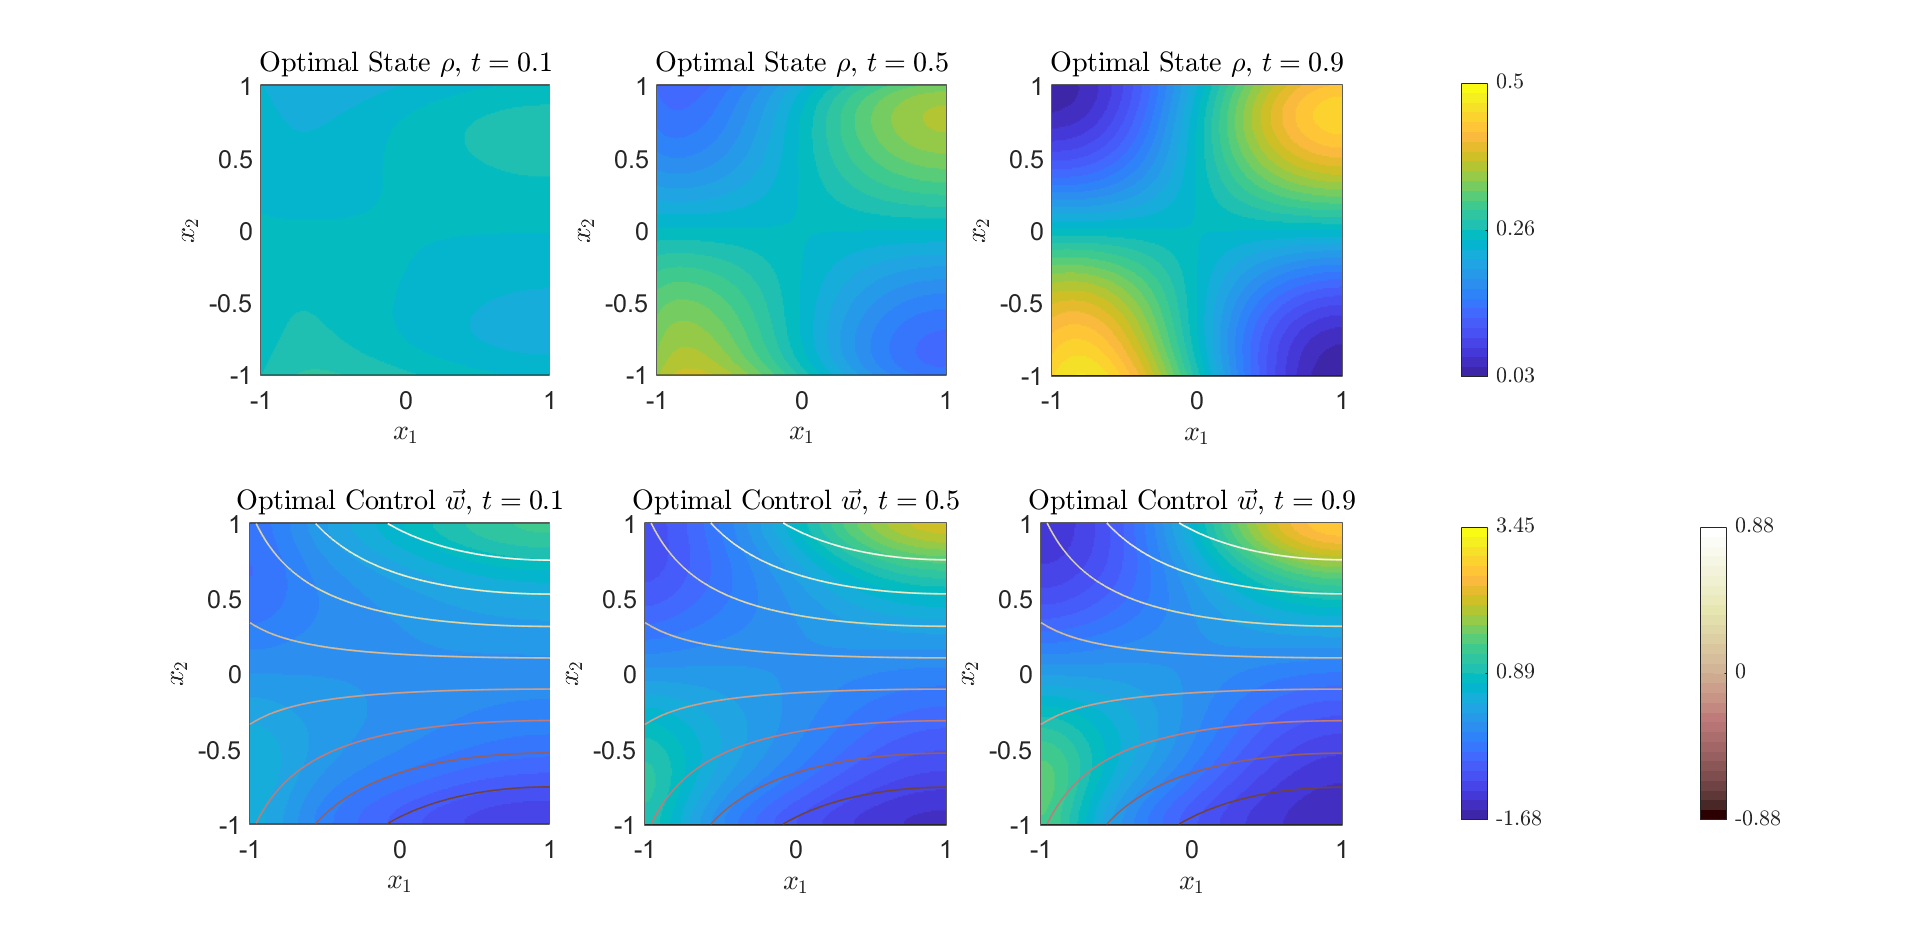
\includegraphics[scale=0.1]{SCNk0.png}
	\caption{Neumann Source Control: Optimal $\rho$ for $\kappa = 0$ and $\beta = 10^{-3}$.} 
	\label{FSCN1}
\end{figure}
\begin{figure}[h]
	\centering
	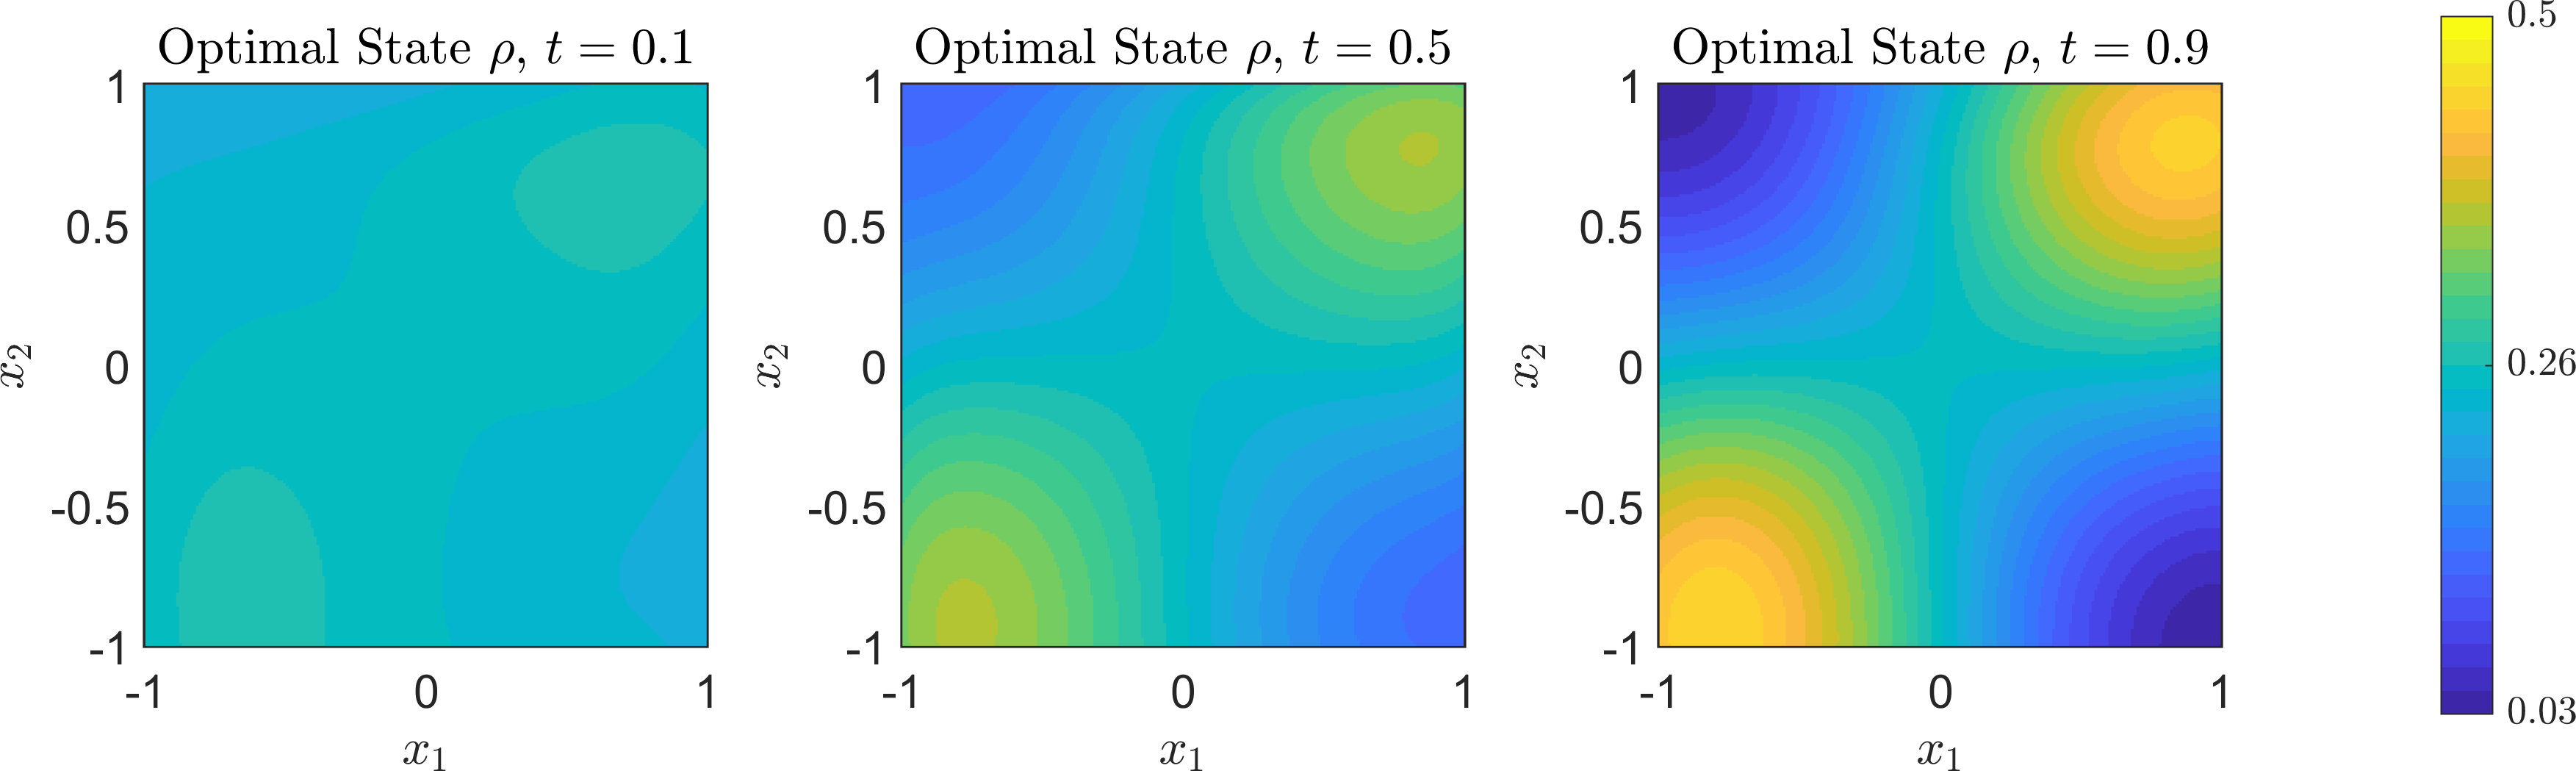
\includegraphics[scale=0.1]{SCNkn1.png}
	\caption{Neumann Source Control: Optimal $\rho$ for $\kappa = -1$ and $\beta = 10^{-3}$.} 
	\label{FSCN2}
\end{figure}
\begin{figure}[h]
	\centering
	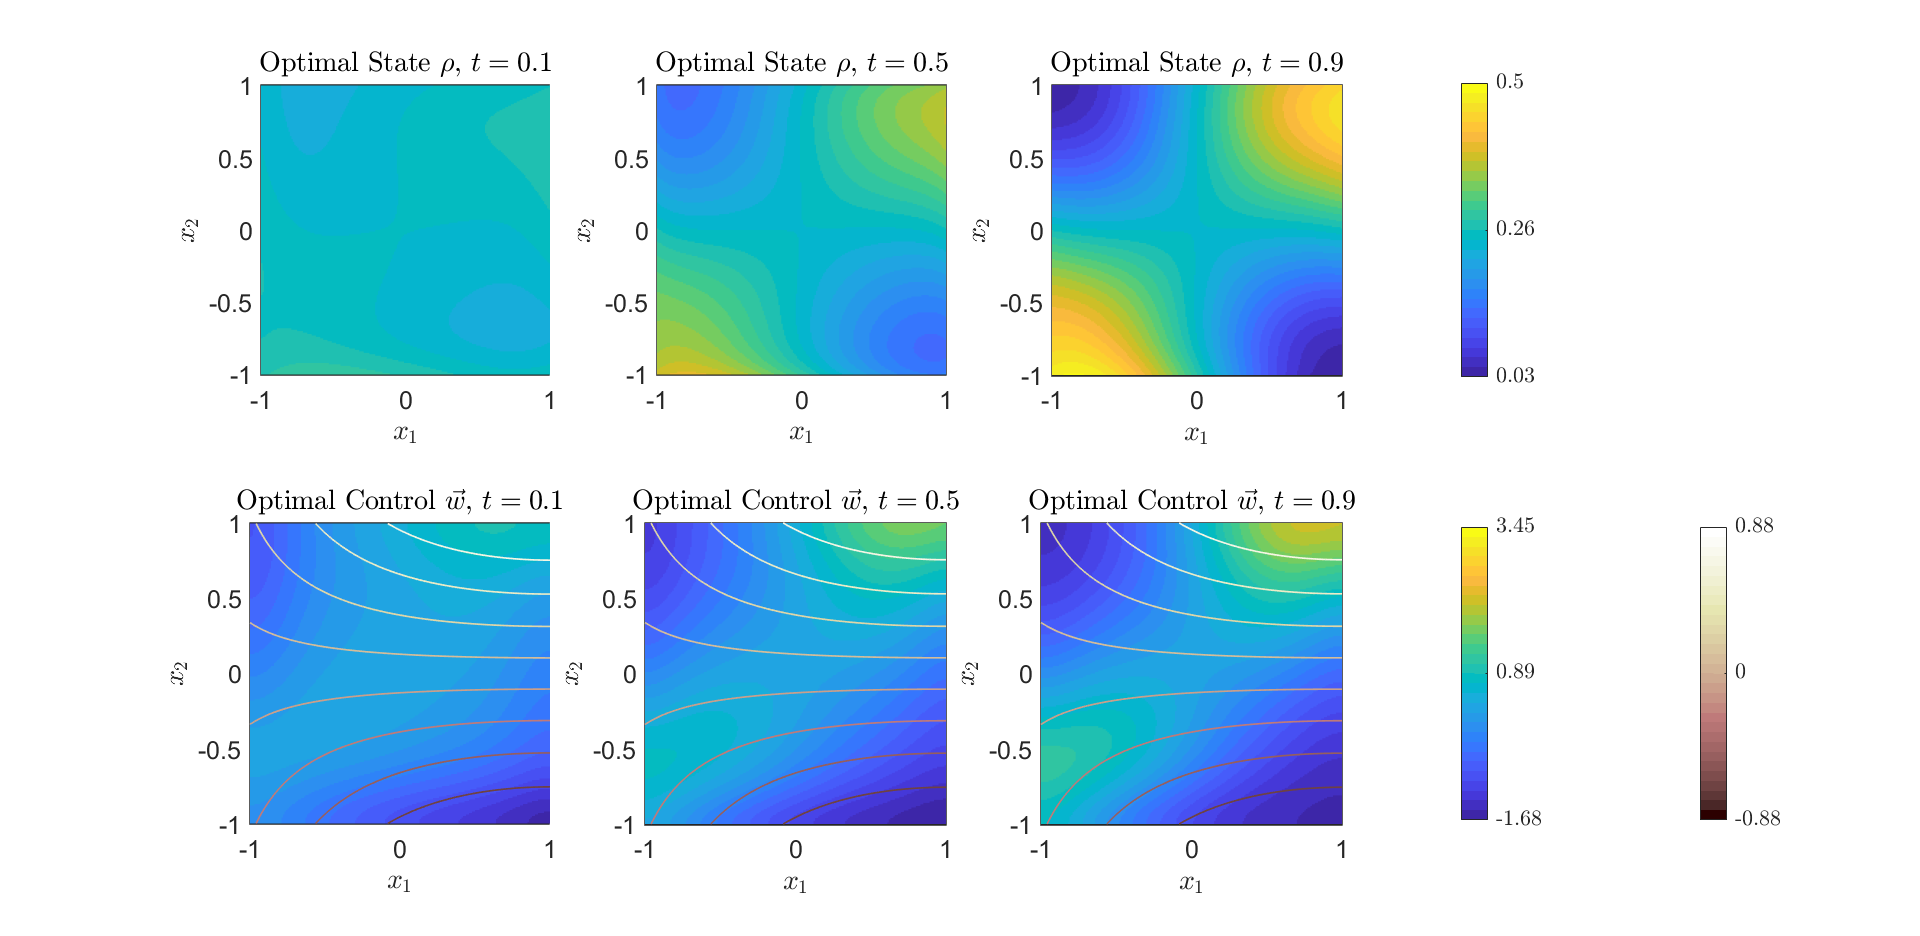
\includegraphics[scale=0.1]{SCNk1.png}
	\caption{Neumann Source Control: Optimal $\rho$ for $\kappa = 1$ and $\beta = 10^{-3}$.} 
	\label{FSCN3}
\end{figure}


\begin{figure}[h]
	\centering
	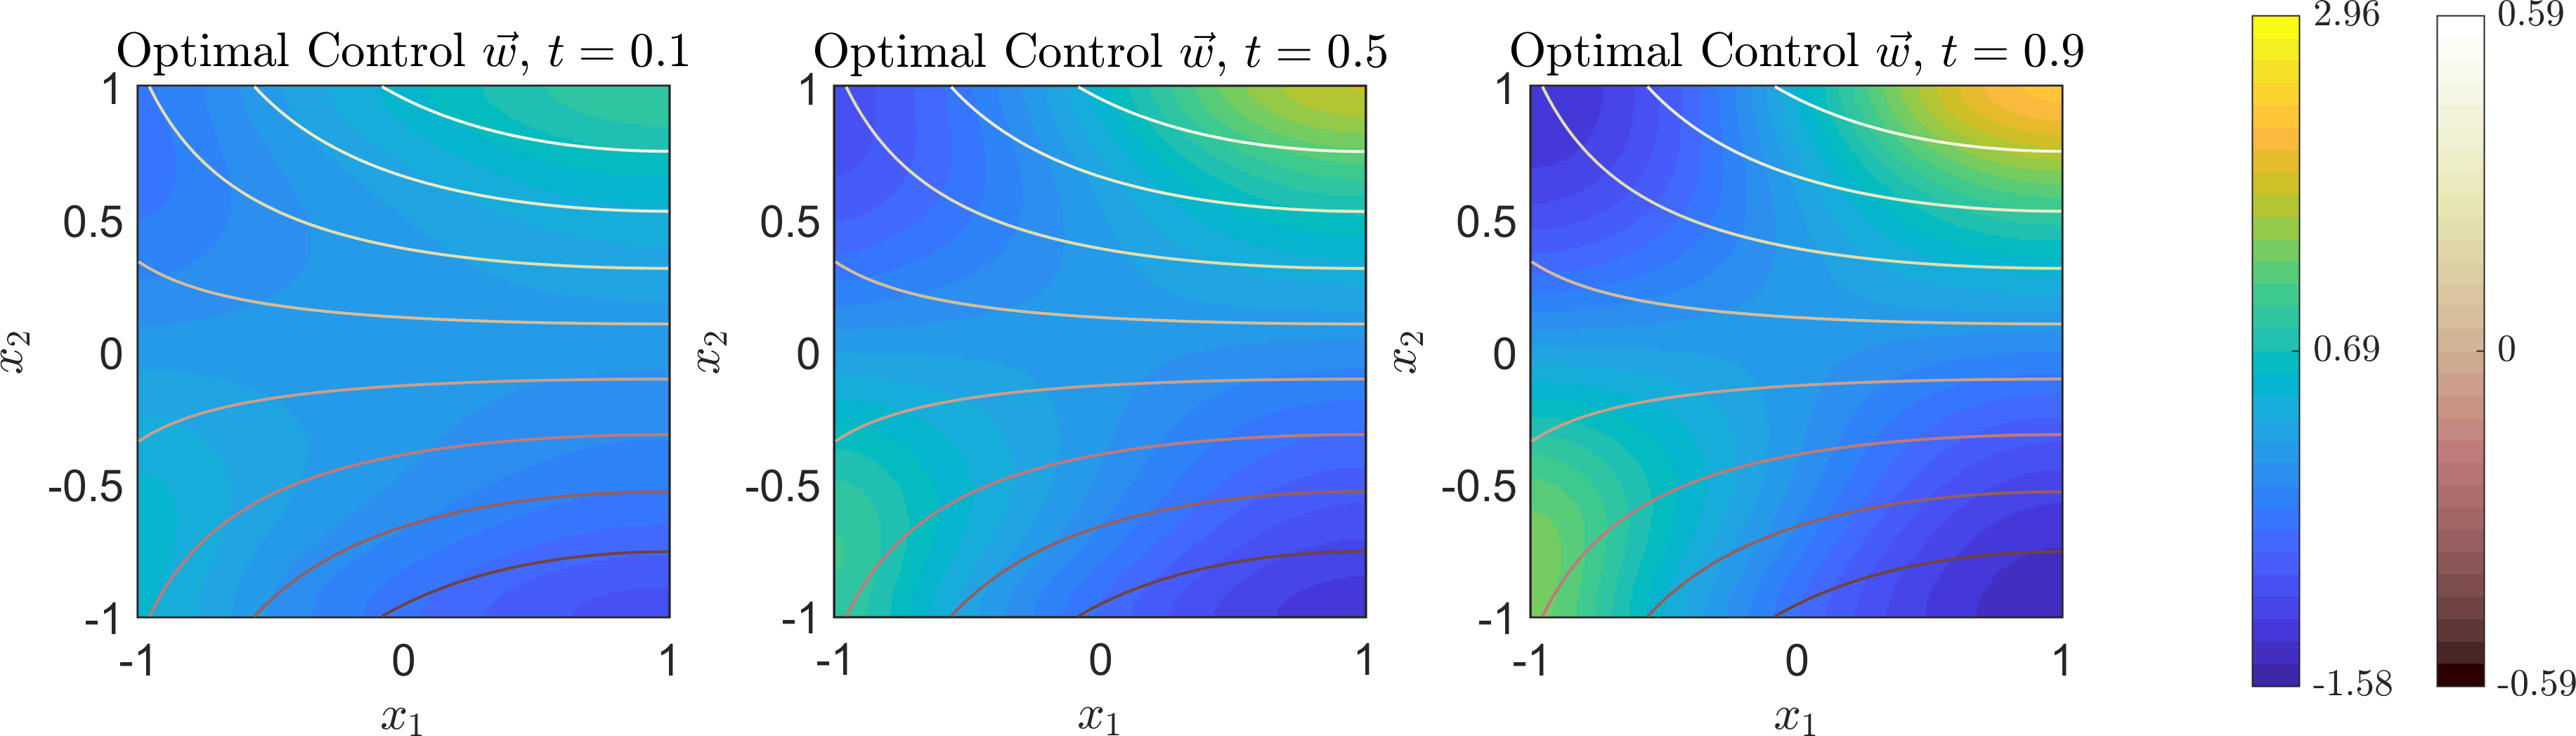
\includegraphics[scale=0.1]{SCNk0c.png}
	\caption{Neumann Source Control: Optimal control for $\kappa = 0$ and $\beta = 10^{-3}$. A contour plot of the external potential \emph{$V_{\text{ext}}$} is superimposed on the control plots for reference, with a corresponding colorbar on the left-hand side.} 
	\label{FSCN1c}
\end{figure}
\begin{figure}[h]
	\centering
	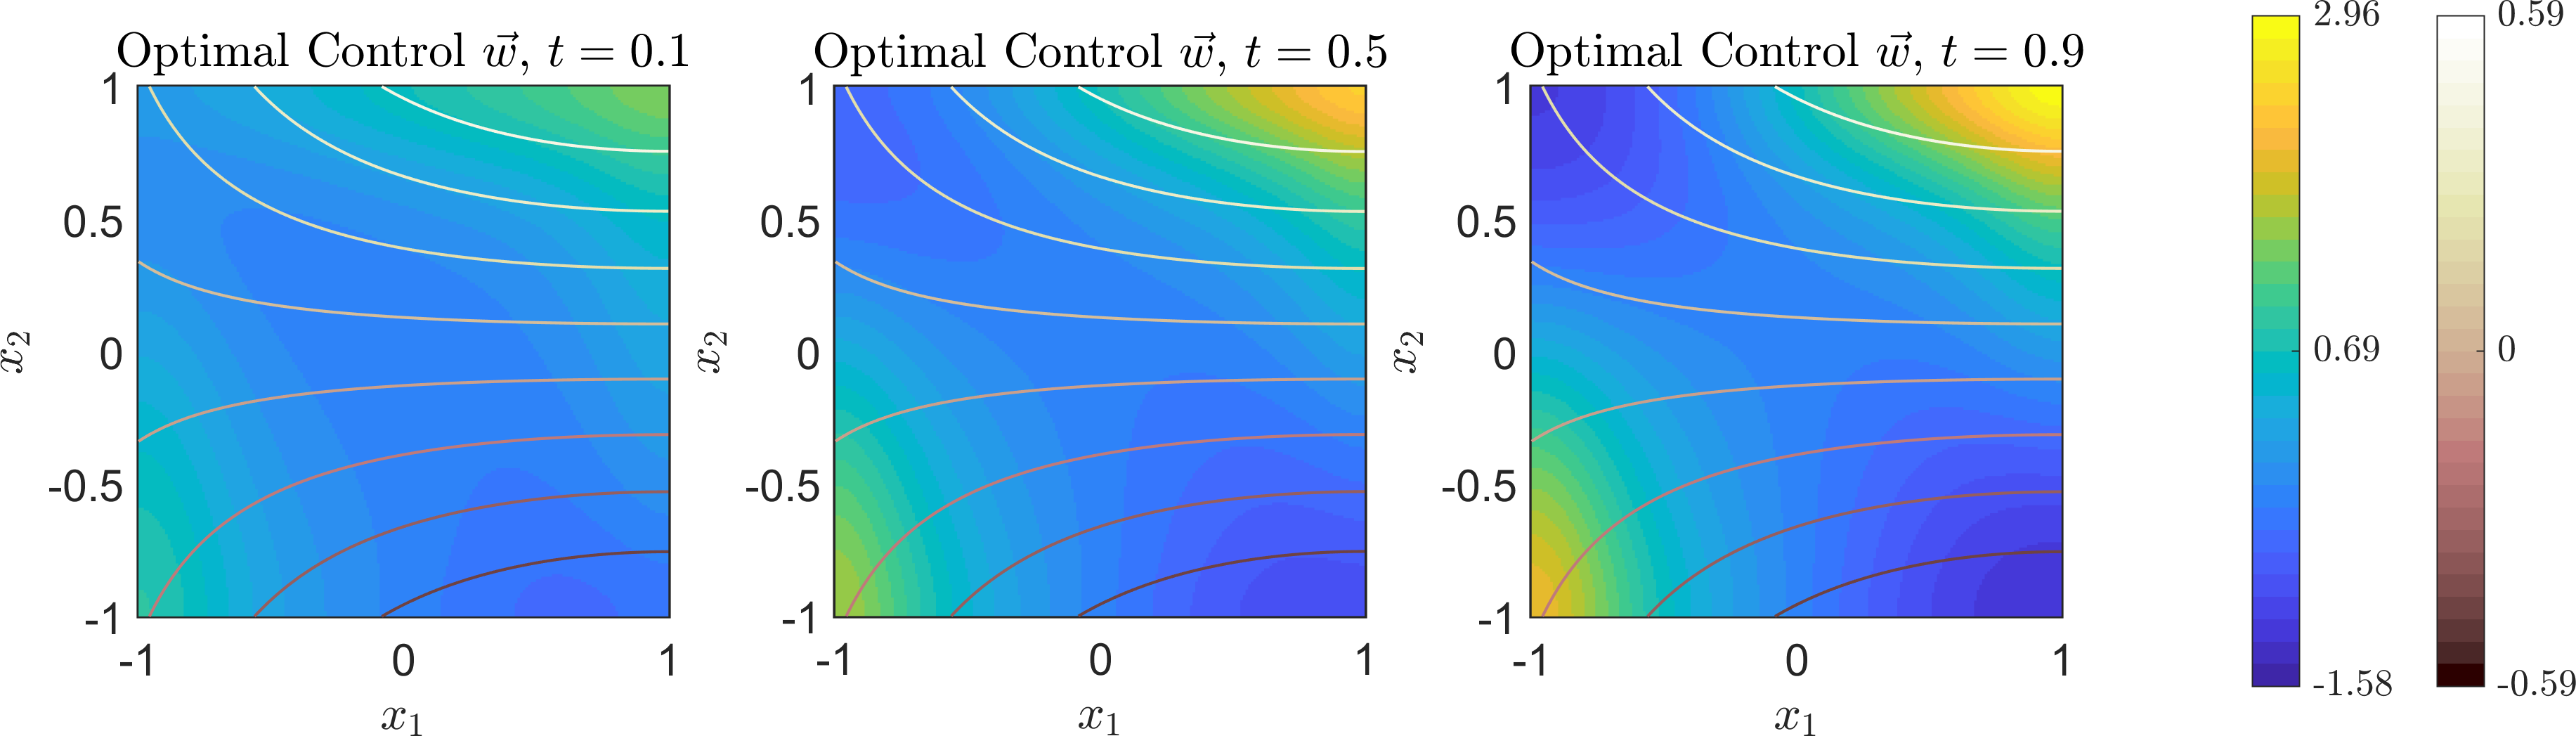
\includegraphics[scale=0.1]{SCNkn1c.png}
	\caption{Neumann Source Control: Optimal control for $\kappa = -1$ and $\beta = 10^{-3}$ and contour plot of the external potential \emph{$V_{\text{ext}}$} as before.} 
	\label{FSCN2c}
\end{figure}
\begin{figure}[h]
	\centering
	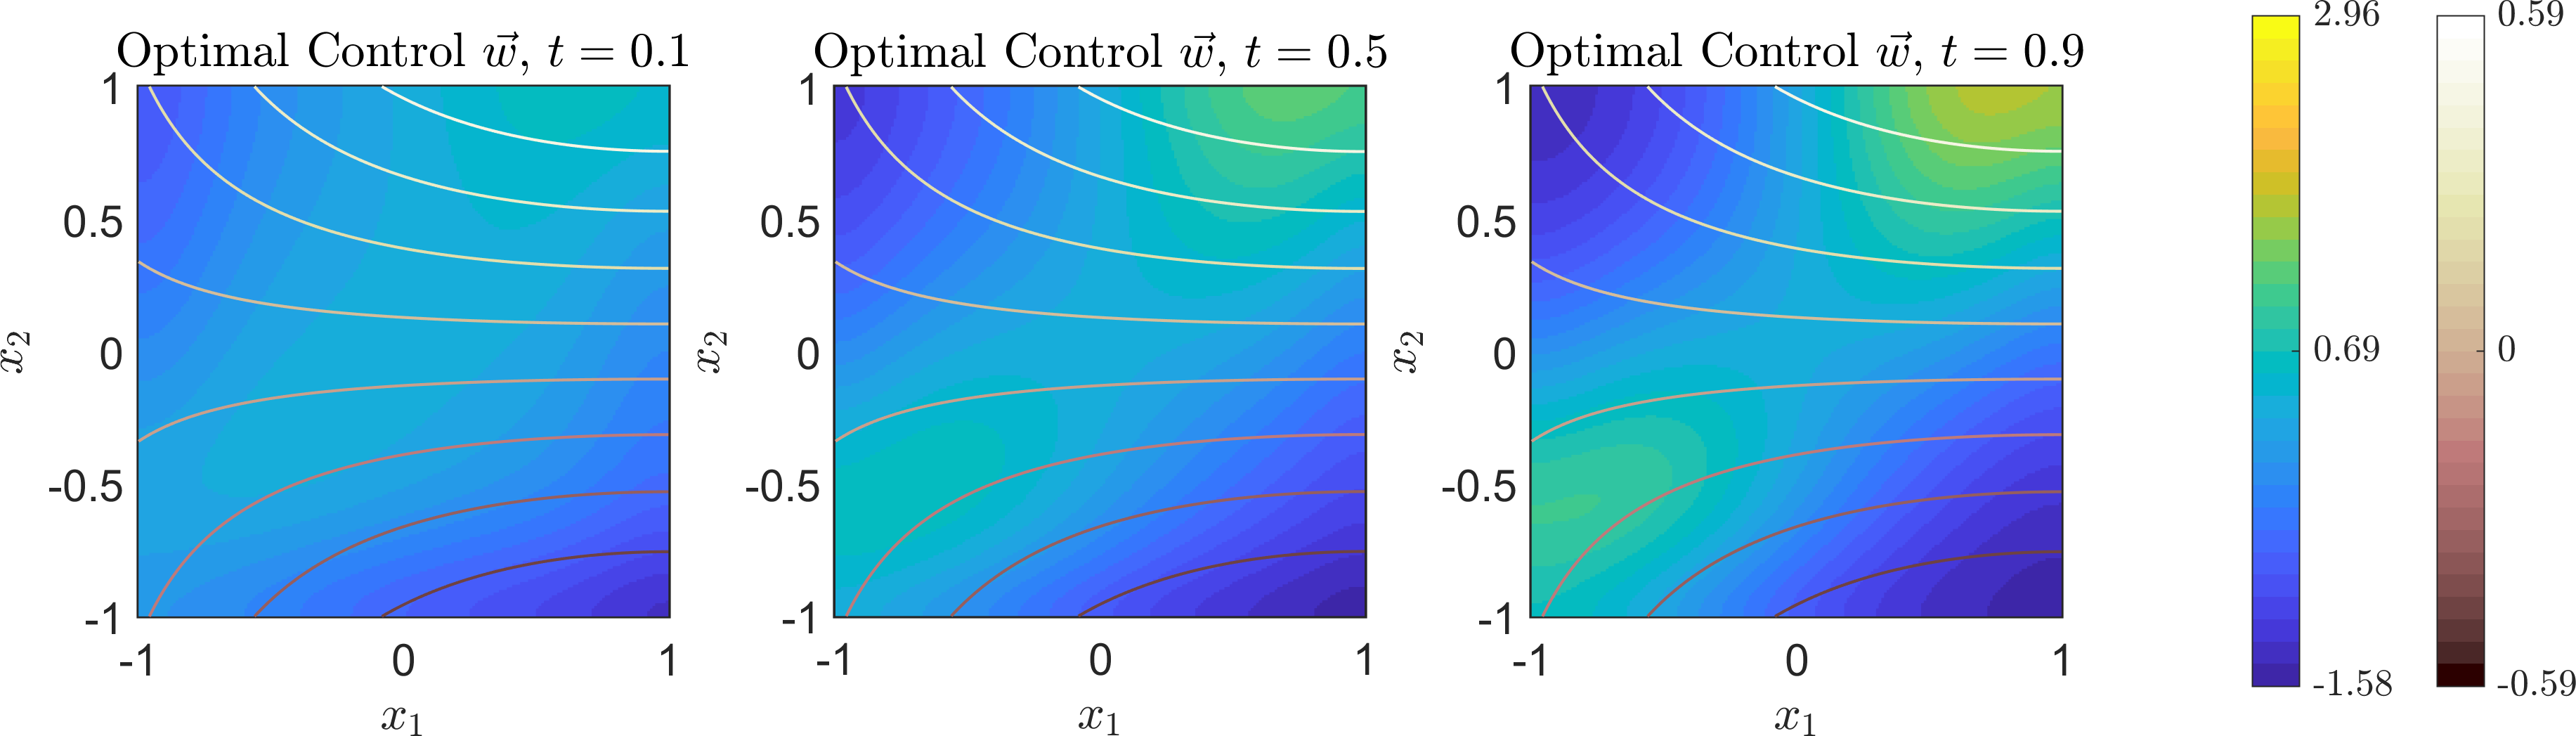
\includegraphics[scale=0.1]{SCNk1c.png}
	\caption{Neumann Source Control: Optimal control for $\kappa = 1$ and $\beta = 10^{-3}$ and contour plot of the external potential \emph{$V_{\text{ext}}$} as before.} 
	\label{FSCN3c}
\end{figure}


\subsubsection{Linear (source) control problem with Dirichlet boundary conditions}
We consider problem \eqref{AdvDiff_Linear} with Dirichlet boundary conditions \eqref{Dirichlet}.
The chosen inputs for our next example are:
\begin{align*}
	\rho_0 &= \frac{1}{4}\cos\left(\frac{\pi x_1}{2}\right)\cos\left(\frac{\pi x_2}{2}\right) + \frac{1}{4}, \quad V_{ext} =  \frac{3}{4}(1-t)\left(-\cos\left(\frac{\pi x_1}{2}\right)\sin\left(\frac{\pi x_2}{2}\right) + 1\right),\\
	\hr &= (1 - t)\left(\frac{1}{4}\cos\left(\frac{\pi x_1}{2}\right)\cos\left(\frac{\pi x_2}{2}\right) + \frac{1}{4}\right) - t\left(\frac{1}{4}\sin\left(\pi x_1\right)\sin\left(\frac{\pi x_2}{2} - \frac{\pi}{2}\right) + \frac{1}{4}\right).
\end{align*}
In this example we choose an external potential, which decays with time. This results in the strongest effect of $V_{ext}$ being visible at earlier times, and none at the final time. Since the external potential is steep around the bottom half of the domain, the mass of particles is not centred in the middle of the domain, but slightly shifted upward. At the same time it can be observed that at $t= 0.1$, the control is applied where the external potential is steep. At later times, the control is mostly applied where the particles are prescribed to accumulate by the desired state $\hr$, which is at the left half of the domain.
When comparing Figure \ref{F2b} displaying results for attractive particles, and Figure \ref{F2c}, showing the effect of repulsive particles, it is evident that the attractive particles cluster more, and therefore less control is needed to achieve the optimal state. The optimal controls corresponding to this are shown in Figures \ref{F2ac}, \ref{F2bc} and \ref{F2cc}.
The results can be seen in Table \ref{TabSCD}.

\begin{table}
\centering
\begin{tabular}{ | c | c || c | c | c | c | c ||}
\hline
\multicolumn{2}{|c||}{}& $\beta = 10^{-5}$ & $\beta = 10^{-3}$ & $\beta = 10^{-1}$ & $\beta = 10^{1}$ & $\beta = 10^{3}$  \\
\hline
\hline
\multirow{2}{*}{$\kappa= \numprint{0}$}  & $\mathcal{J}_{uc}$ & $\numprint{1.50e-2}$ & $\numprint{1.50e-2}$ & $\numprint{1.50e-2}$ & $\numprint{1.50e-2}$ & $\numprint{1.50e-2}$\\
 & $\mathcal{J}_c$ & $\numprint{3.40e-5}$ & $\numprint{1.92e-3}$ & $\numprint{1.36e-2}$ & $\numprint{1.50e-2}$ & $\numprint{1.50e-2}$\\
\hline
\multirow{2}{*}{$\kappa= \numprint{1}$}  & $\mathcal{J}_{uc}$ & $\numprint{2.06e-2}$ & $\numprint{2.06e-2}$ & $\numprint{2.06e-2}$ & $\numprint{2.06e-2}$ & $\numprint{2.06e-2}$\\
 & $\mathcal{J}_c$ & $\numprint{4.27e-5}$ & $\numprint{2.49e-3}$ & $\numprint{1.85e-2}$ & $\numprint{2.06e-2}$ & $\numprint{2.06e-2}$\\
\hline
\multirow{2}{*}{$\kappa= \numprint{-1}$}  & $\mathcal{J}_{uc}$ & $\numprint{1.27e-2}$ & $\numprint{1.27e-2}$ & $\numprint{1.27e-2}$ & $\numprint{1.27e-2}$ & $\numprint{1.27e-2}$\\
 & $\mathcal{J}_c$ & $\numprint{2.88e-5}$ & $\numprint{1.61e-3}$ & $\numprint{1.18e-2}$ & $\numprint{1.27e-2}$ & $\numprint{1.27e-2}$\\
\hline
\end{tabular}
\caption{Source Control Dirichlet Problem: Cost $\mathcal{J}_{uc}$ of applying no control (i.e., $\vec{w} = \vec{0}$)and optimal control cost $\mathcal{J}_{c}$ for a range of values of the interaction strength $\kappa$ and regularization parameter $\beta$. The value of $\mathcal J_{c}$ for $\beta = 10^{-5}$ is of order $10^{-5}$. Note that for $\beta = 10$, the cost functionals differ by $10{-5}$, while for $\beta = 10^3$ they differ by $10^{-7}$ for $\kappa = 0$ and $\kappa = 1$ and by $10^{-8}$ for $\kappa = -1$.}
\label{TabSCD}
\end{table}
\begin{figure}[h]
	\centering
	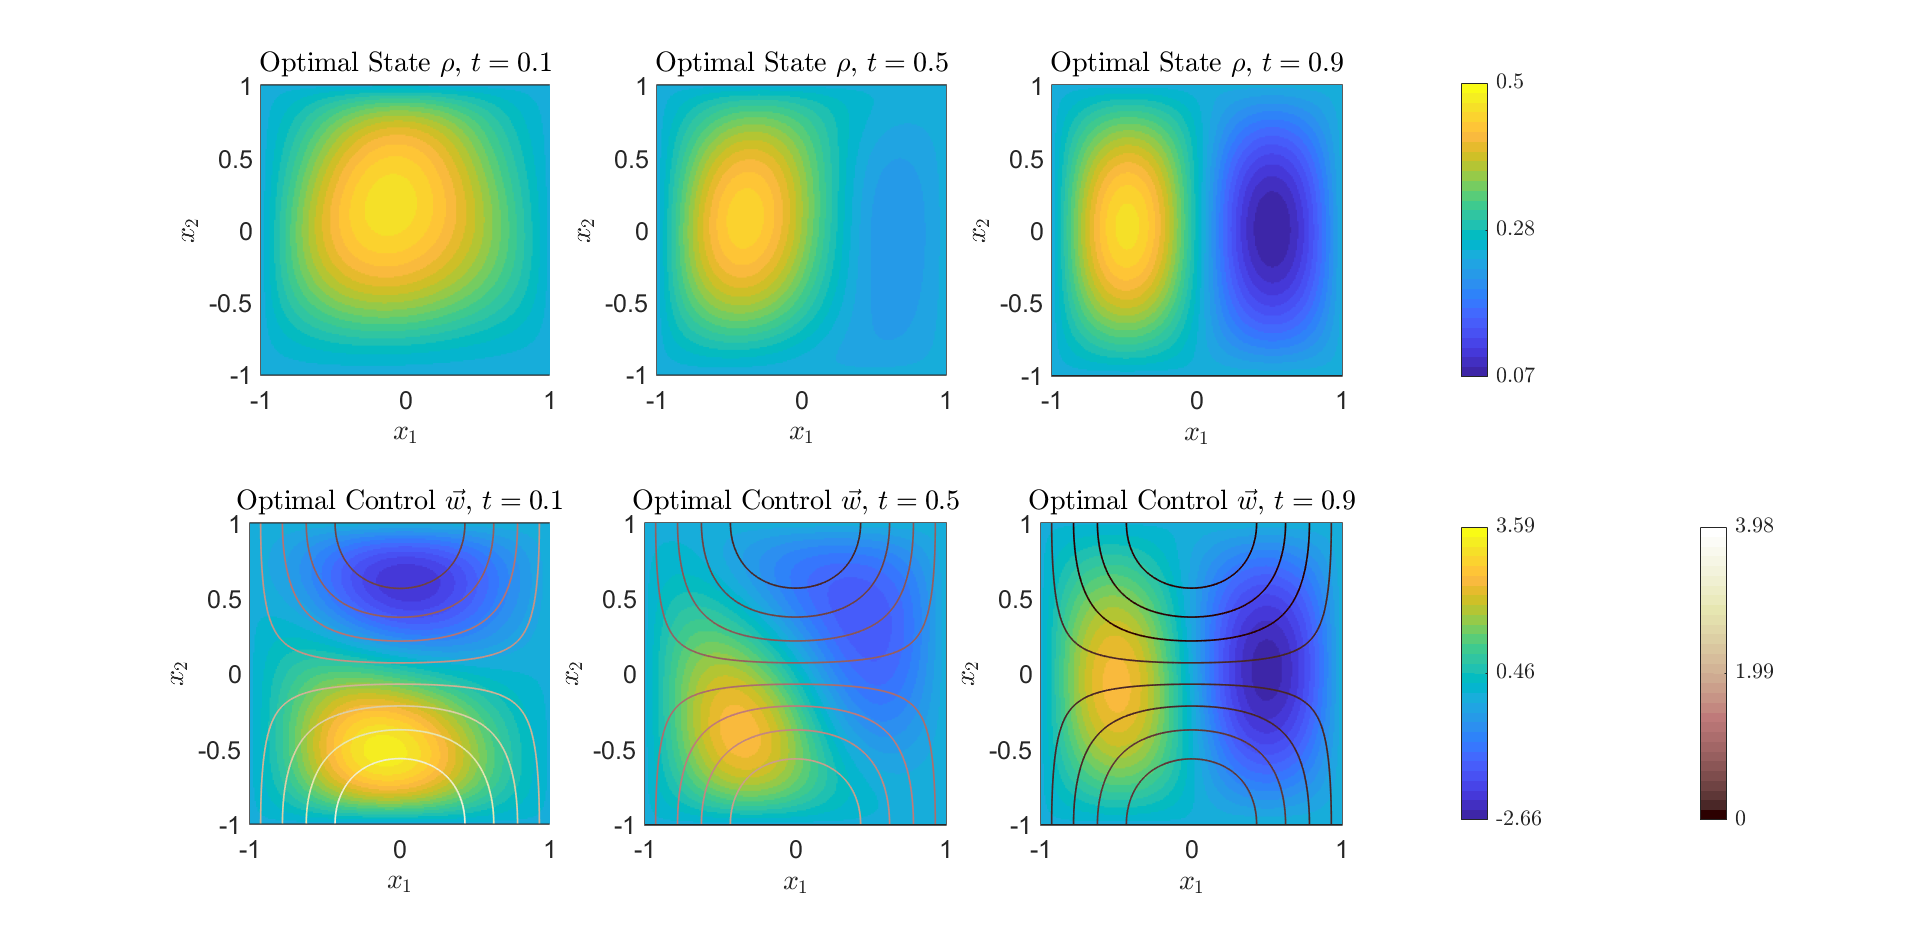
\includegraphics[scale=0.1]{SCDk0.png}
	\caption{Dirichlet Source Control: Optimal $\rho$ for $\kappa = 0$ and $\beta = 10^{-3}$.} 
	\label{F2a}
\end{figure}
\begin{figure}[h]
	\centering
	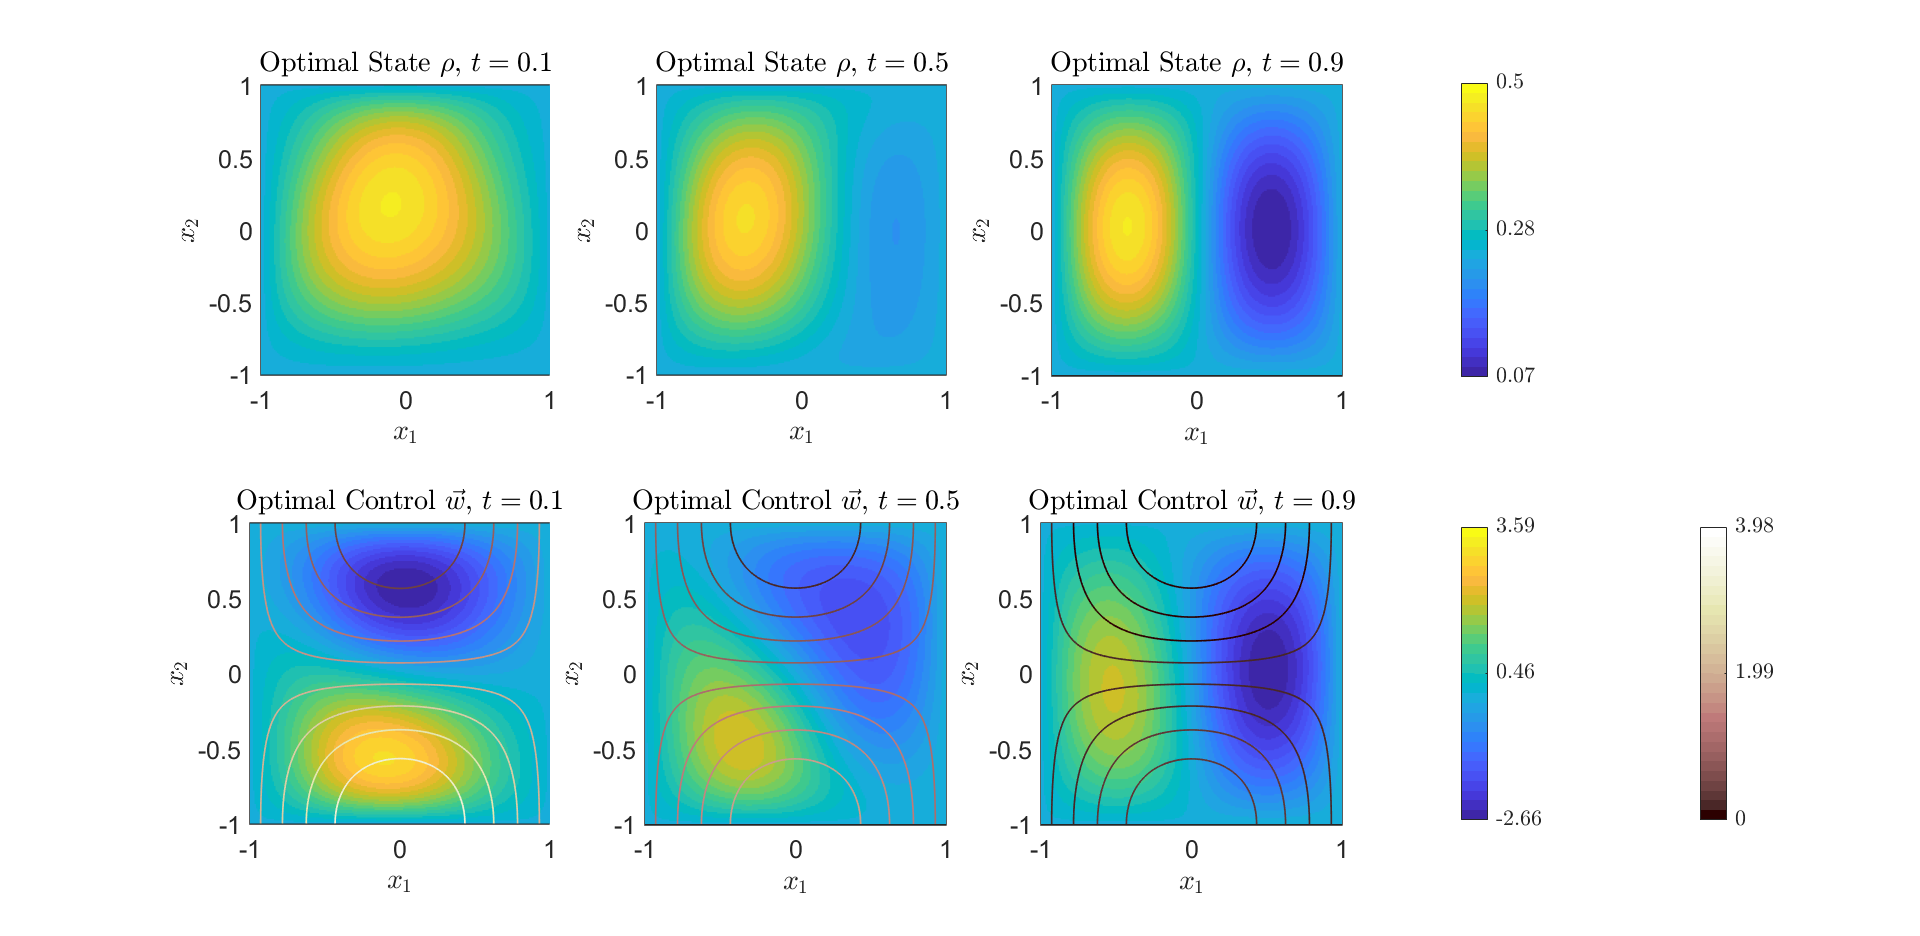
\includegraphics[scale=0.1]{SCDkn1.png}
	\caption{Dirichlet Source Control: Optimal $\rho$ for $\kappa = -1$ and $\beta = 10^{-3}$.} 
	\label{F2b}
\end{figure}
\begin{figure}[h]
	\centering
	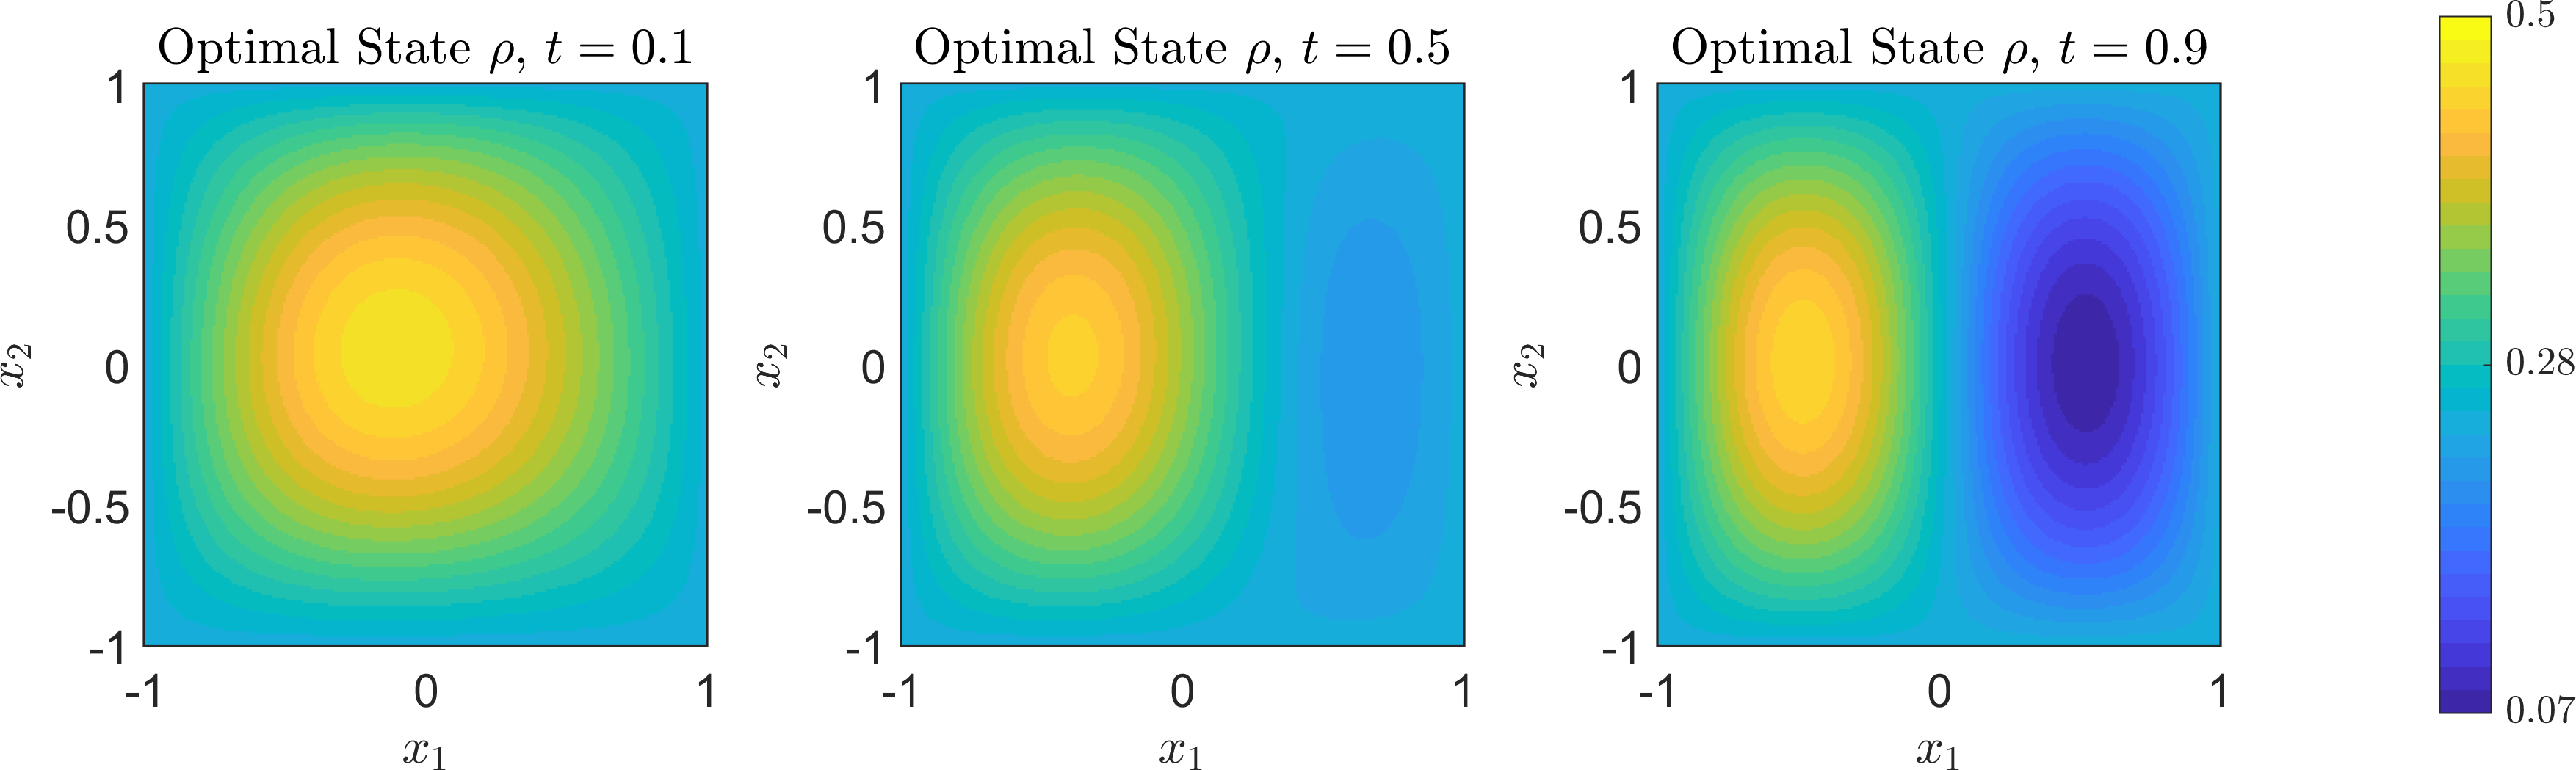
\includegraphics[scale=0.1]{SCDk1.png}
	\caption{Dirichlet Source Control: Optimal $\rho$ for $\kappa = 1$ and $\beta = 10^{-3}$.} 
	\label{F2c}
\end{figure}

	\begin{figure}[h]
	\centering
	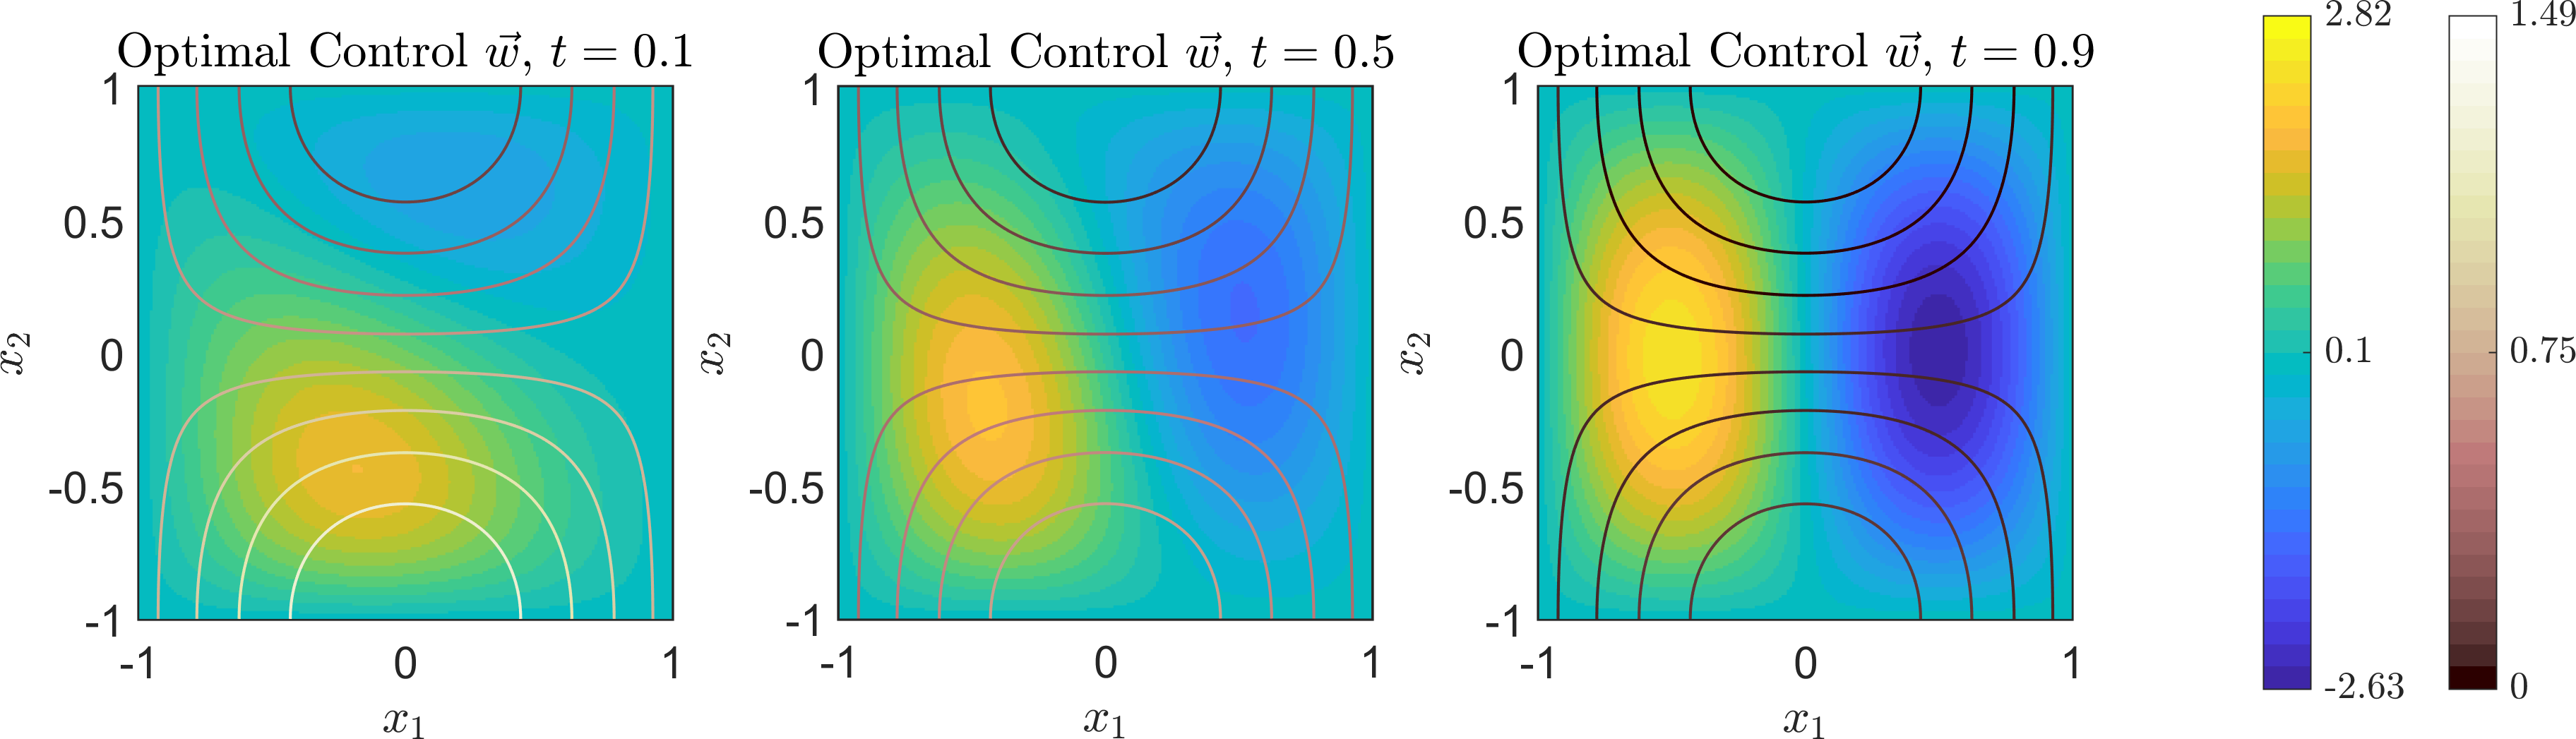
\includegraphics[scale=0.1]{SCDk0c.png}
	\caption{Dirichlet Source Control: Optimal control for $\kappa = 0$ and $\beta = 10^{-3}$. A contour plot of the external potential \emph{$V_{\text{ext}}$} is superimposed on the control plots for reference, with a corresponding colorbar on the left-hand side.} 
	\label{F2ac}
\end{figure}
\begin{figure}[h]
	\centering
	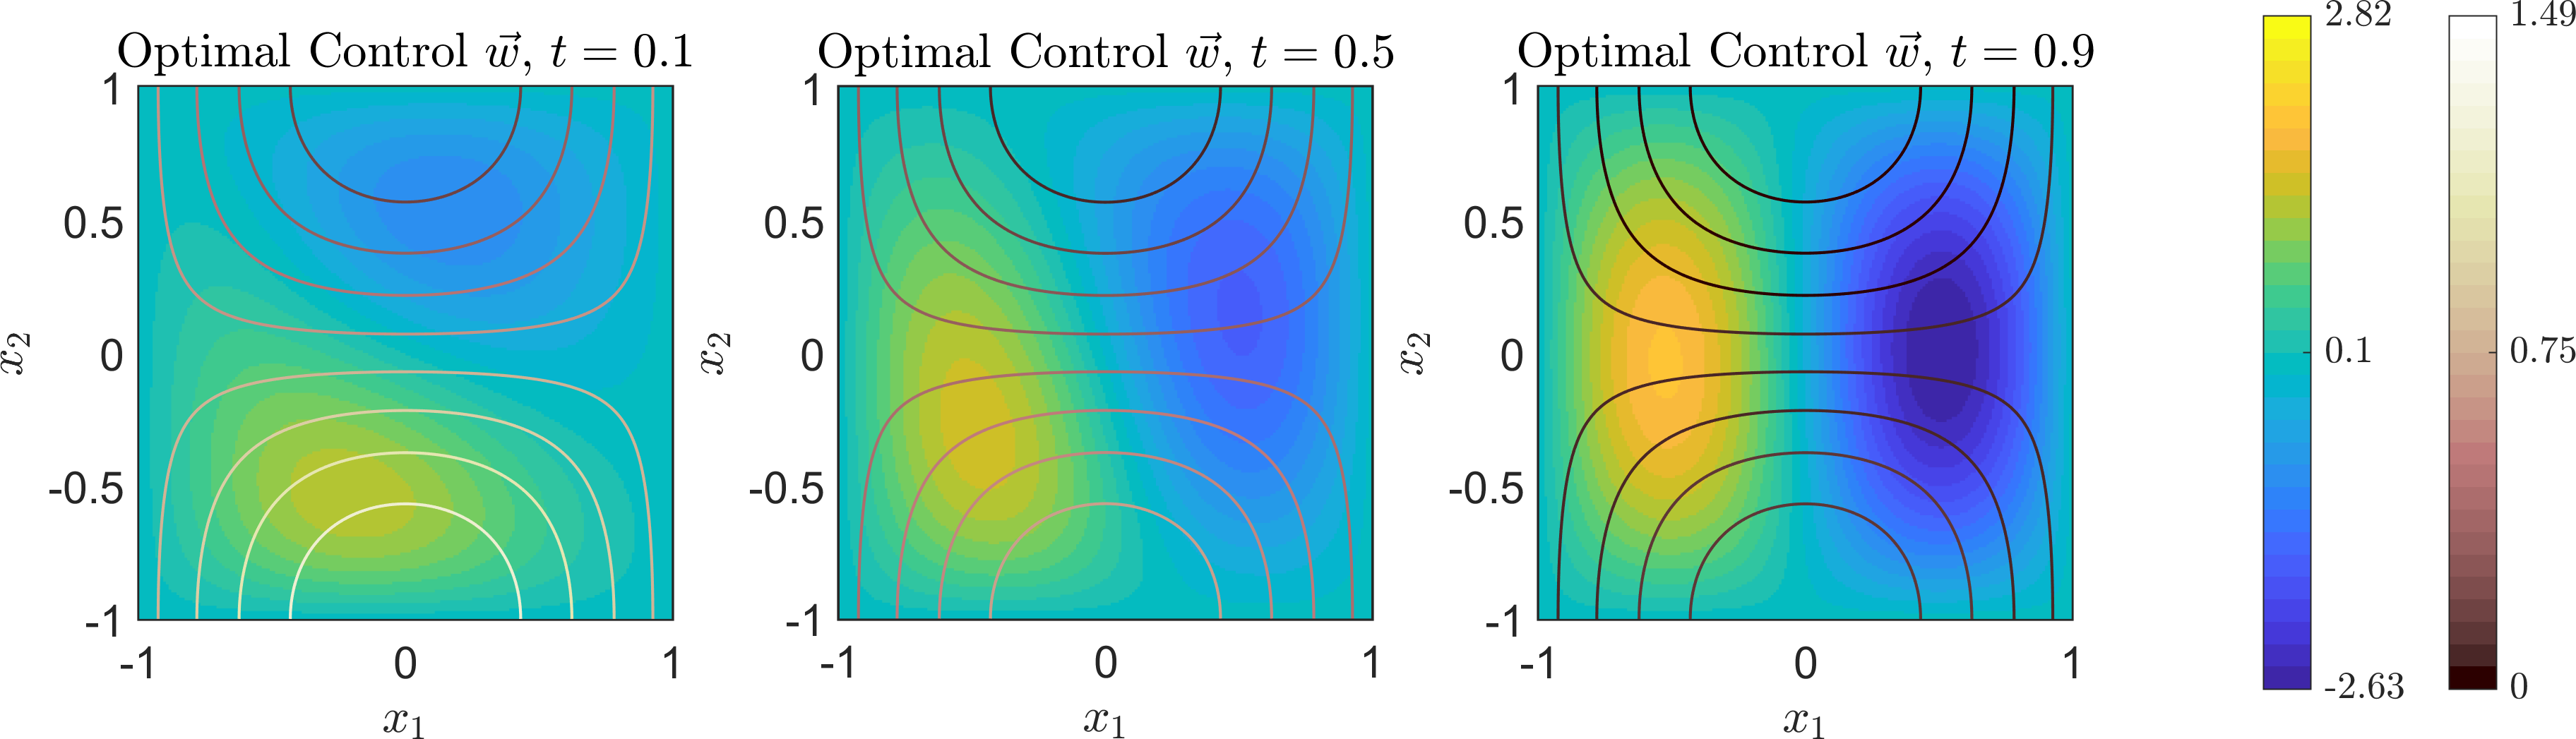
\includegraphics[scale=0.1]{SCDkn1c.png}
	\caption{Dirichlet Source Control: Optimal control for $\kappa = -1$ and $\beta = 10^{-3}$ and contour plot of the external potential \emph{$V_{\text{ext}}$} as before.} 
	\label{F2bc}
\end{figure}
\begin{figure}[h]
	\centering
	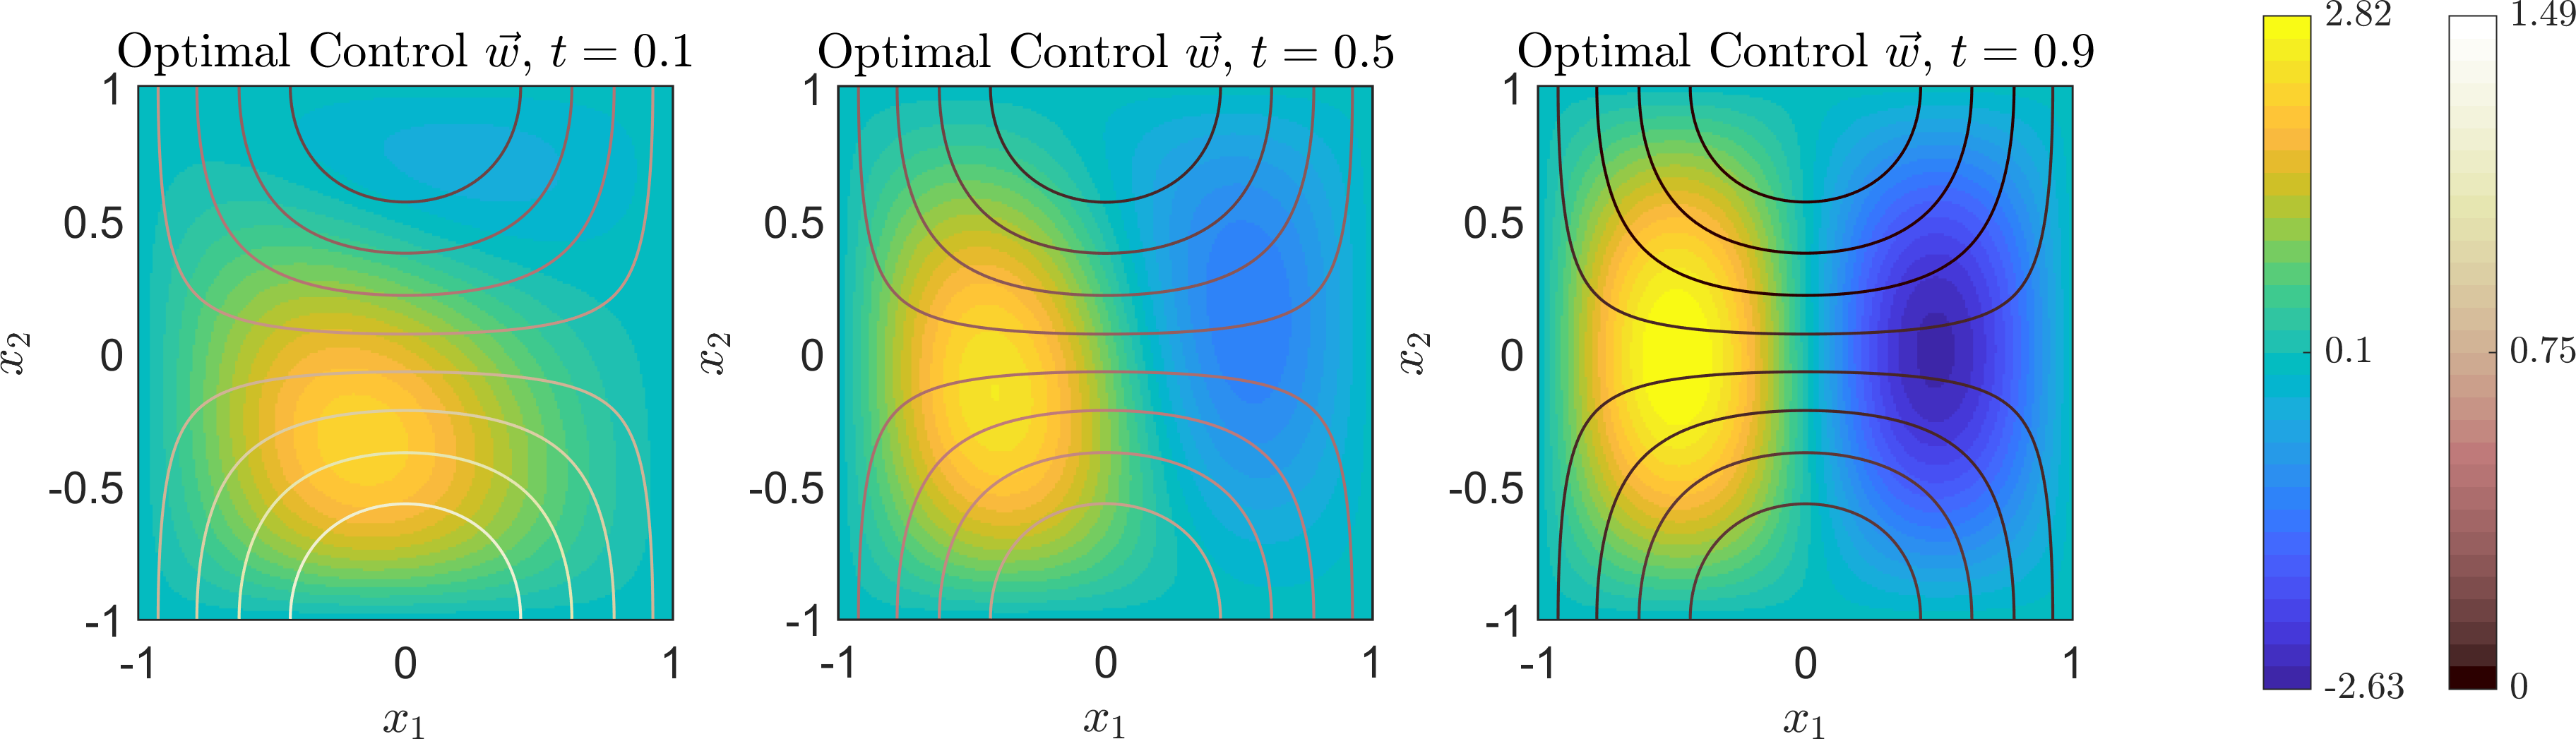
\includegraphics[scale=0.1]{SCDk1c.png}
	\caption{Dirichlet Source Control: Optimal control for $\kappa = 1$ and $\beta = 10^{-3}$ and contour plot of the external potential \emph{$V_{\text{ext}}$} as before.} 
	\label{F2cc}
\end{figure}



\subsubsection{Non-linear (flow) control problem with no-flux boundary conditions}
Next an example of system \eqref{AdvDiff} is considered with no-flux boundary conditions \eqref{NoFlux}.
The inputs here are:
\begin{align*}
	\rho_0 &= \frac{1}{4}, \quad \hr = \frac{1}{4}(1-t) + t\frac{1}{1.3791}\exp{\left(-2\left(\left(x_1+0.2\right)^2 + \left(x_2+0.2\right)^2\right)\right)},\\
	V_{ext} &= \left(\left(x_1 + 0.3\right)^2 - 1\right)\left(\left(x_1-0.4\right)^2 - 0.5\right)
	\left(\left(x_2 + 0.3\right)^2 - 1\right)\left(\left(x_2-0.4\right)^2 - 0.5\right).
\end{align*}
The numerical results for this example are displayed in Table \ref{TabFCN}. The results are illustrated for $\beta = 10^{-3}$ and $\kappa = -1$. Figures \ref{F3a}, \ref{F3b} and \ref{F3c} demonstrate the effect of $V_{\text{ext}}$ on the state, while Figures \ref{F3ac}, \ref{F3bc} and \ref{F3cc} display the corresponding controls. At earlier times, the particle mass accumulates in regions with potential wells and the areas where the potential is steep are avoided. In the Figures it can be observed very clearly that the control is driving the particle distribution to the desired state. It is noticeable that the control does not act uniformly around the peak of the desired state, but also acts strongly in the area between the location of the desired peak and the point $(-1,1)$. This is due to the external potential being steep in this area and more control is needed to reach the desired state than in other parts of the domain. 
((++ Comment on Cost update example! ++))

\begin{table}
\centering
\begin{tabular}{ | c | c || c | c | c | c | c ||}
\hline
\multicolumn{2}{|c||}{}& $\beta = 10^{-5}$ & $\beta = 10^{-3}$ & $\beta = 10^{-1}$ & $\beta = 10^{1}$ & $\beta = 10^{3}$  \\
\hline
\hline
\multirow{2}{*}{$\kappa= \numprint{0}$}  & $\mathcal{J}_{uc}$ & $\numprint{2.67e-2}$ & $\numprint{2.67e-2}$ & $\numprint{2.67e-2}$ & $\numprint{2.67e-2}$ & $\numprint{2.67e-2}$\\
 & $\mathcal{J}_c$ & $\numprint{8.23e-5}$ & $\numprint{3.87e-3}$ & $\numprint{2.50e-2}$ & $\numprint{2.67e-2}$ & $\numprint{2.67e-2}$\\
\hline
\multirow{2}{*}{$\kappa= \numprint{1}$}  & $\mathcal{J}_{uc}$ & $\numprint{3.29e-2}$ & $\numprint{3.29e-2}$ & $\numprint{3.29e-2}$ & $\numprint{3.29e-2}$ & $\numprint{3.29e-2}$\\
 & $\mathcal{J}_c$ & $\numprint{1.16e-4}$ & $\numprint{5.44e-3}$ & $\numprint{3.13e-2}$ & $\numprint{3.29e-2}$ & $\numprint{3.29e-2}$\\
\hline
\multirow{2}{*}{$\kappa= \numprint{-1}$}  & $\mathcal{J}_{uc}$ & $\numprint{2.09e-2}$ & $\numprint{2.09e-2}$ & $\numprint{2.09e-2}$ & $\numprint{2.09e-2}$ & $\numprint{2.09e-2}$\\
 & $\mathcal{J}_c$ & $\numprint{5.71e-5}$ & $\numprint{2.63e-3}$ & $\numprint{1.92e-2}$ & $\numprint{2.09e-2}$ & $\numprint{2.09e-2}$\\
\hline
\end{tabular}
\caption{Flow Control No-Flux Problem: Cost when $\vec{w}=\vec{0}$ and optimal control cost for a range of $\kappa$, $\beta$. Note that for $\beta = 10$, the cost functionals differ by $10^{-5}$, while for $\beta = 10^3$ they differ by $10^{-7}$ (++ two in the wrong direction ++).}
\label{TabFCN}
\end{table}
\begin{figure}[h]
	\centering
	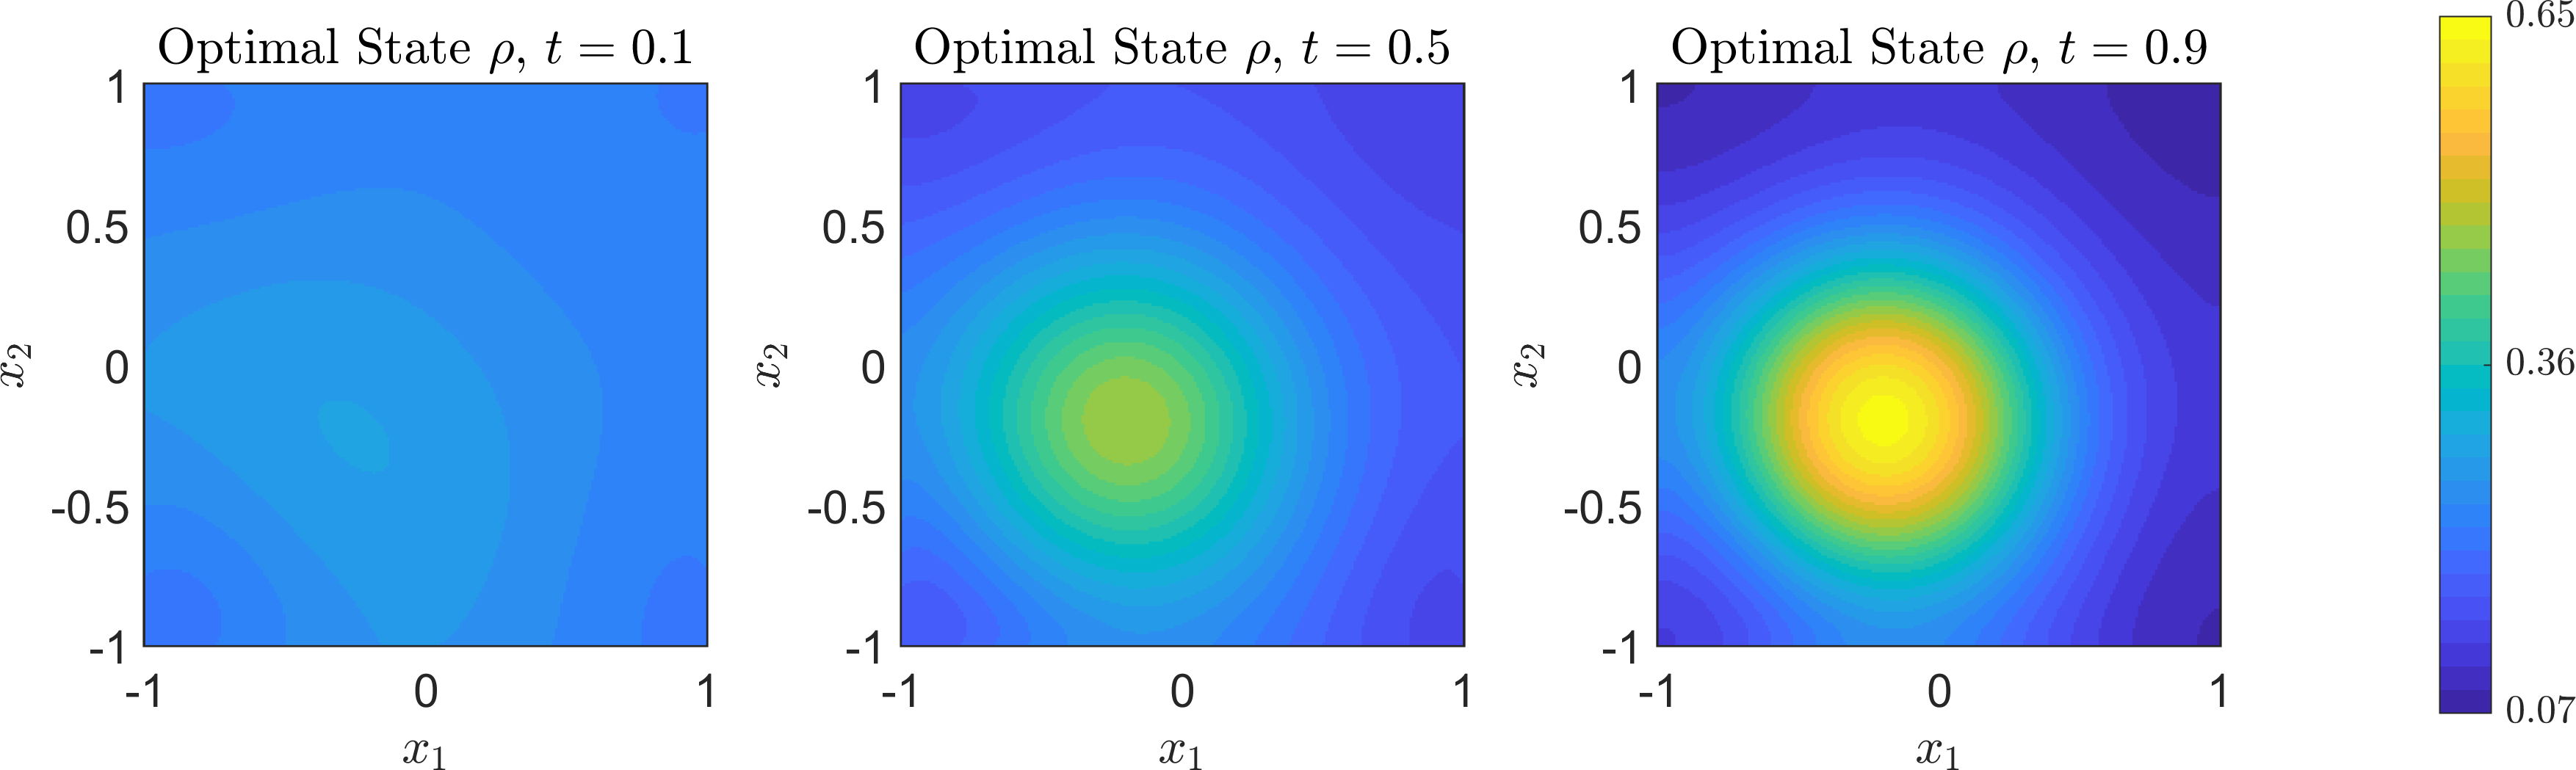
\includegraphics[scale=0.1]{FCNk0.png}
	\caption{Neumann Flow Control: Optimal $\rho$ for $\kappa = 0$ and $\beta = 10^{-3}$.} 
	\label{F3a}
\end{figure}
\begin{figure}[h]
	\centering
	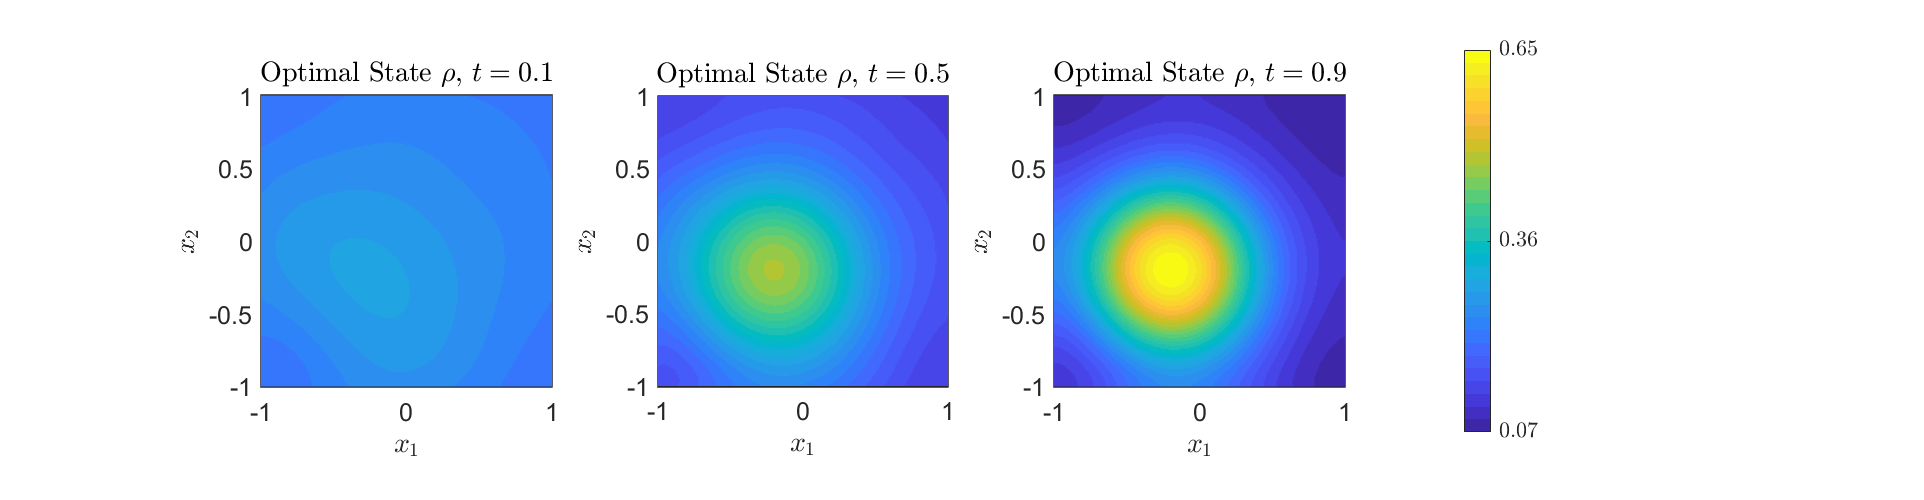
\includegraphics[scale=0.1]{FCNkn1.png}
	\caption{Neumann Flow Control: Optimal $\rho$ for $\kappa = -1$ and $\beta = 10^{-3}$.} 
	\label{F3b}
\end{figure}
\begin{figure}[h]
	\centering
	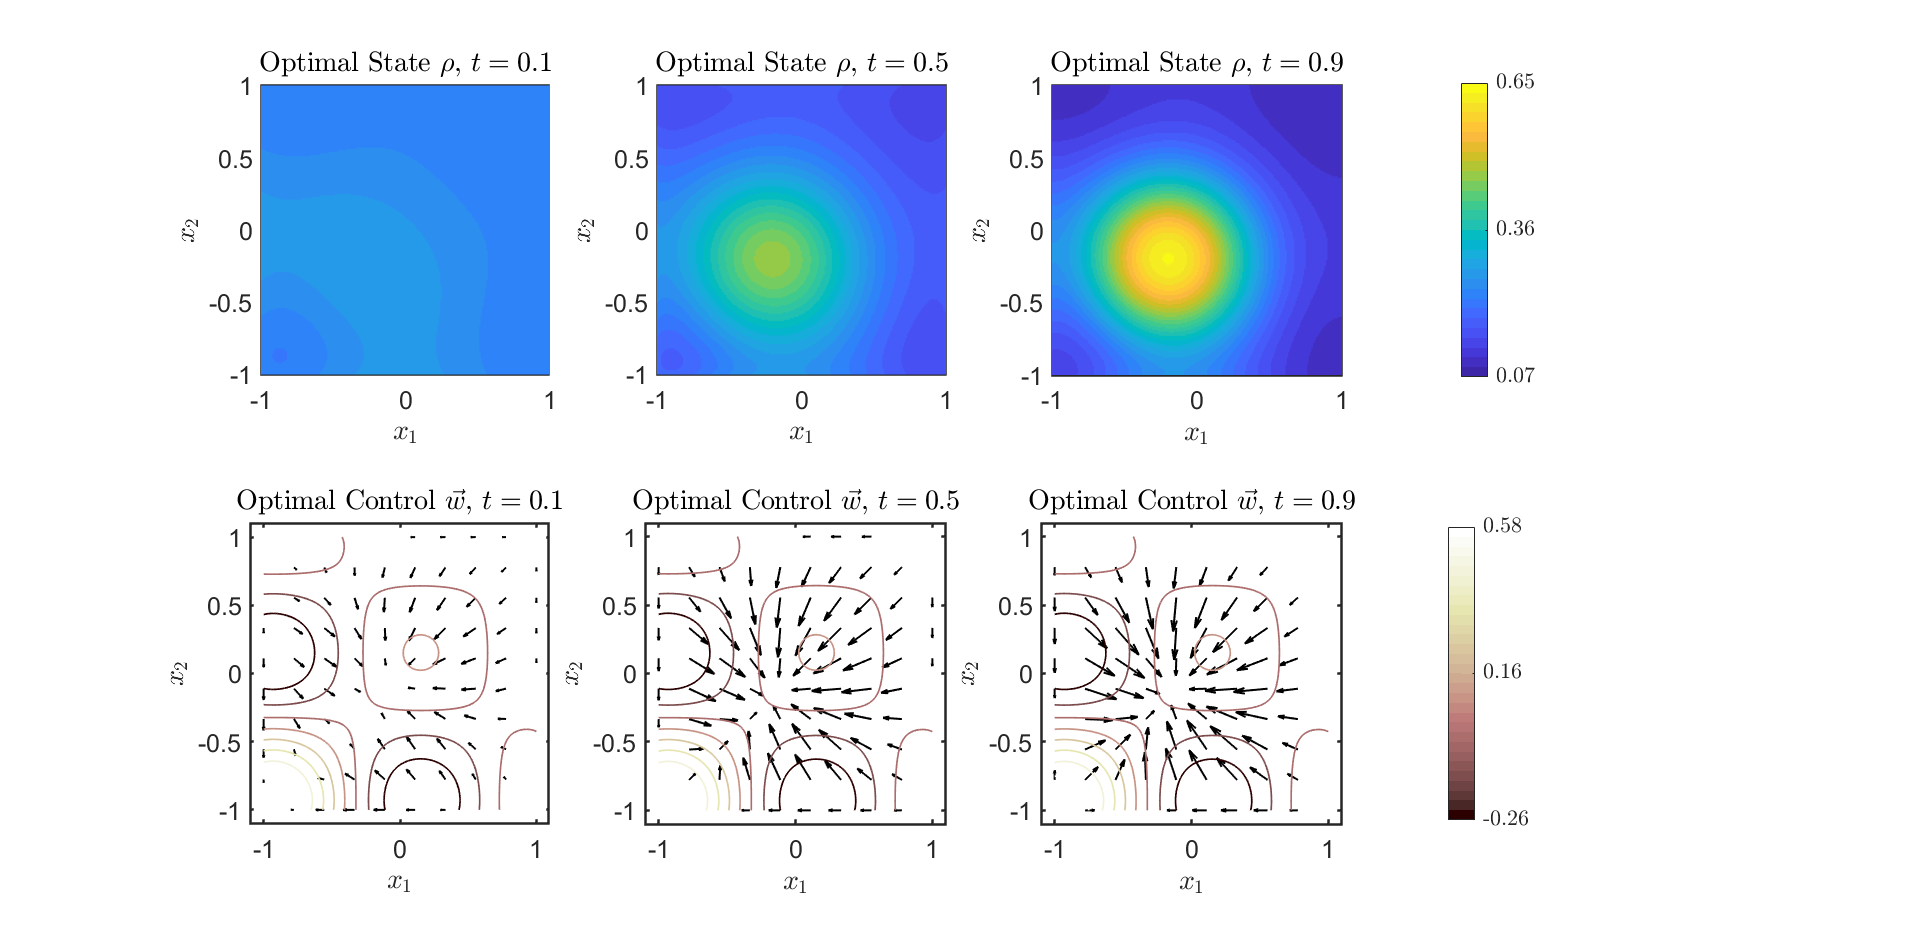
\includegraphics[scale=0.1]{FCNk1.png}
	\caption{Neumann Flow Control: Optimal $\rho$ for $\kappa = 1$ and $\beta = 10^{-3}$.} 
	\label{F3c}
\end{figure}


\begin{figure}[h]
	\centering
	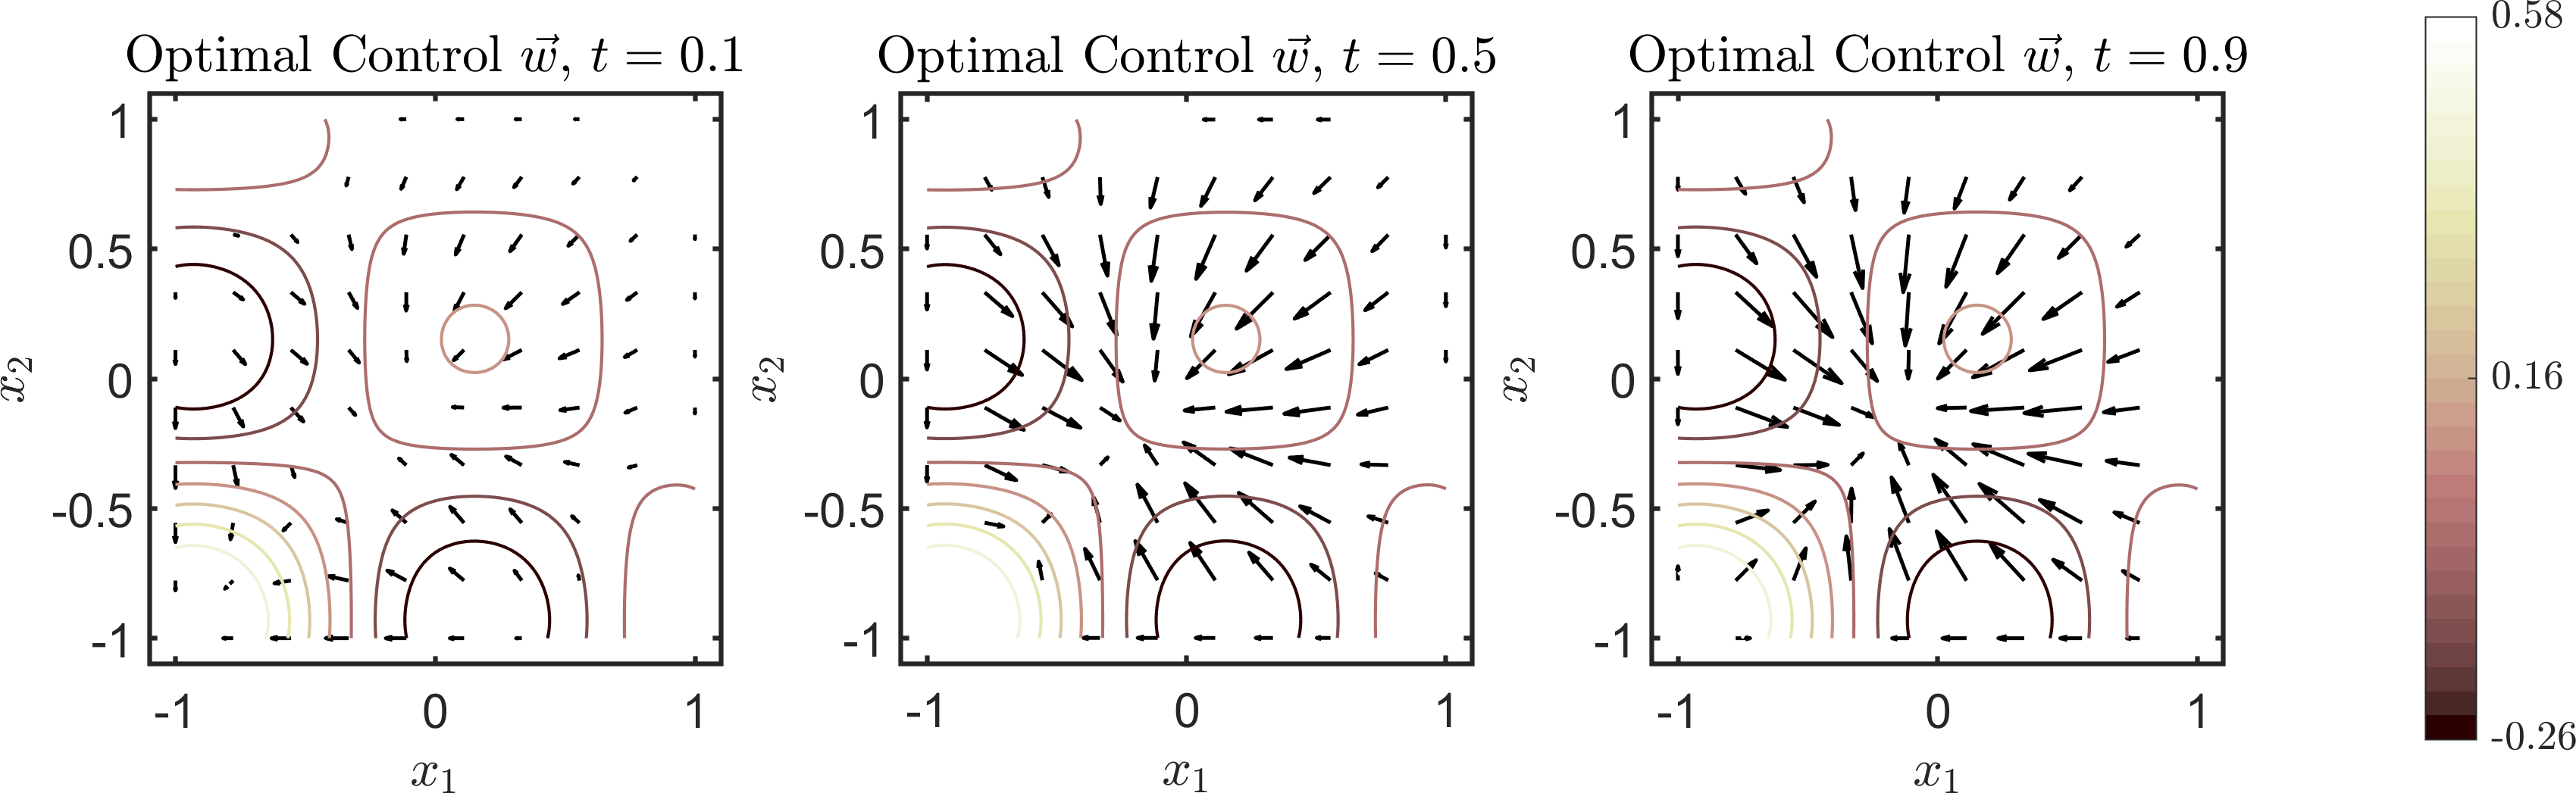
\includegraphics[scale=0.1]{FCNk0c.png}
	\caption{Neumann Flow Control: Optimal control for $\kappa = 0$ and $\beta = 10^{-3}$. A contour plot of the external potential \emph{$V_{\text{ext}}$} is superimposed on the control plots for reference, with a corresponding colorbar on the left-hand side.} 
	\label{F3ac}
\end{figure}
\begin{figure}[h]
	\centering
	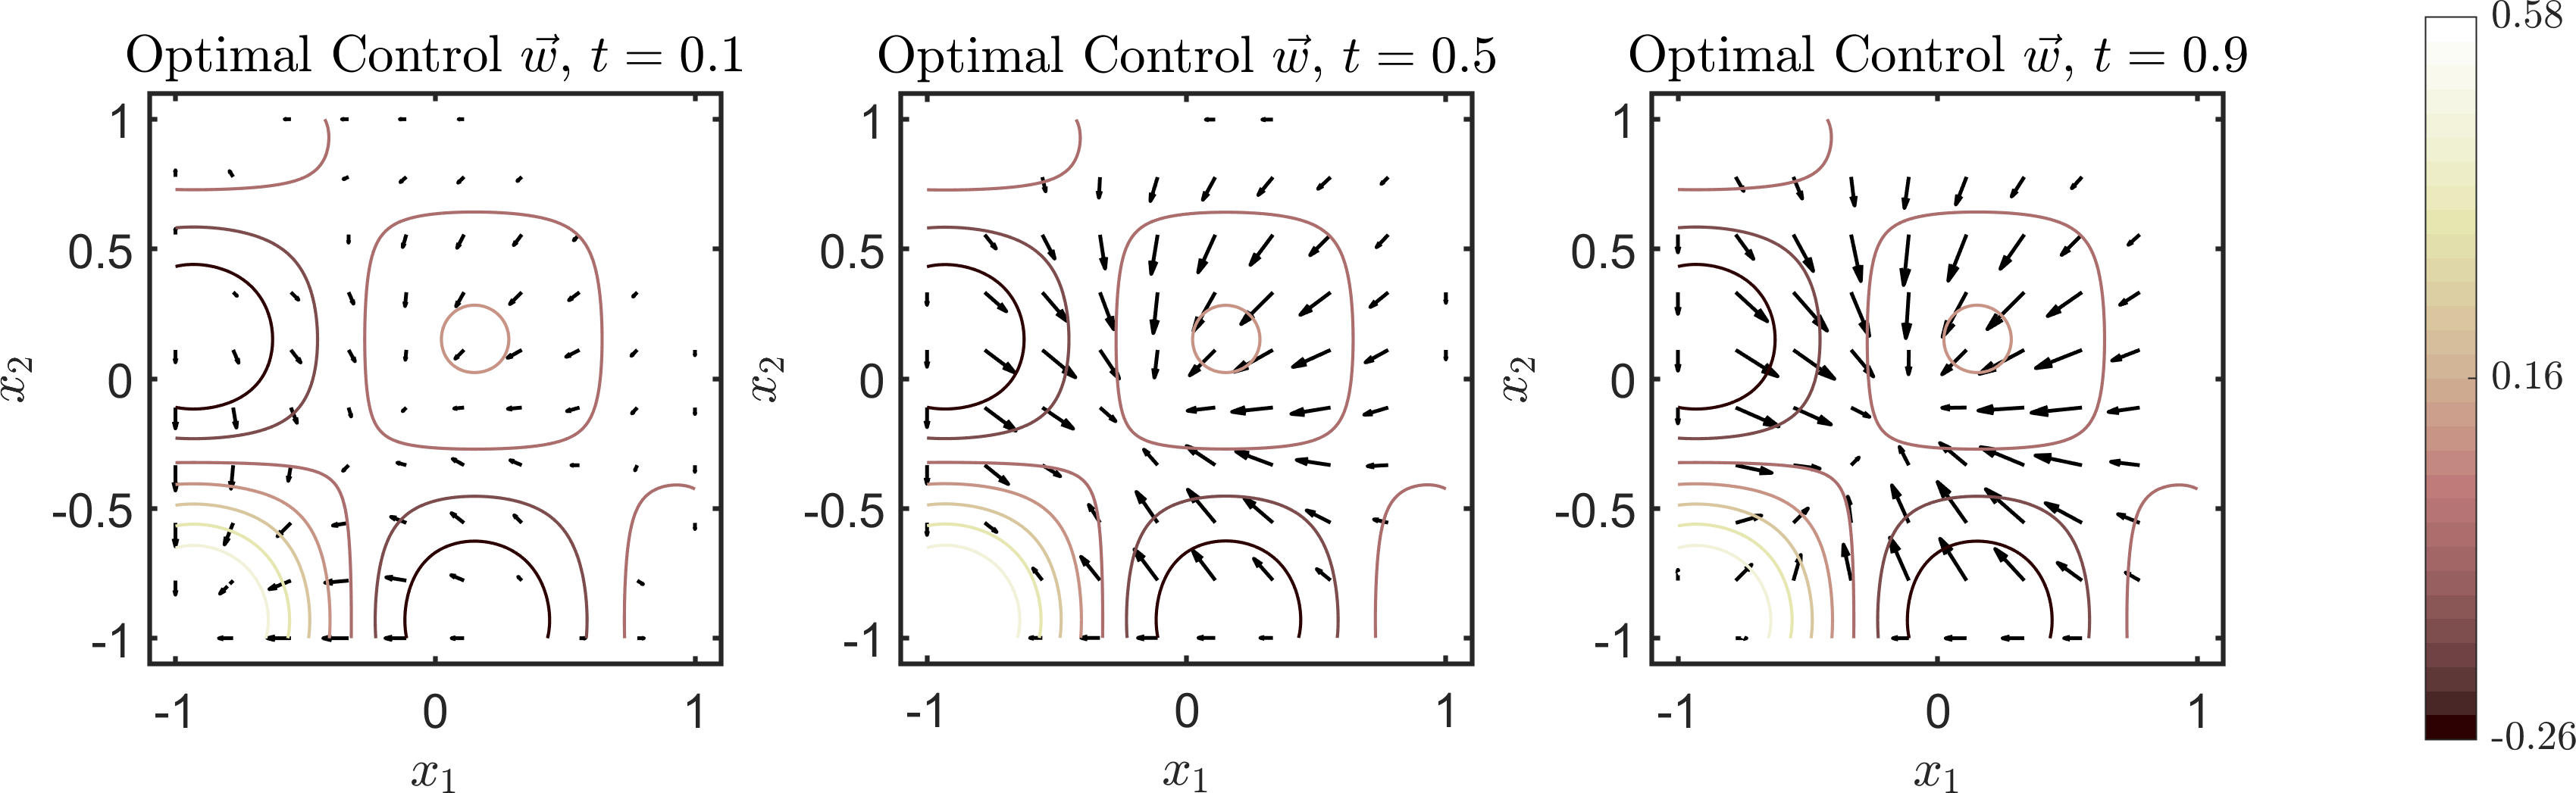
\includegraphics[scale=0.1]{FCNkn1c.png}
	\caption{Neumann Flow Control: Optimal control for $\kappa = -1$ and $\beta = 10^{-3}$ and contour plot of the external potential \emph{$V_{\text{ext}}$} as before.} 
	\label{F3bc}
\end{figure}
\begin{figure}[h]
	\centering
	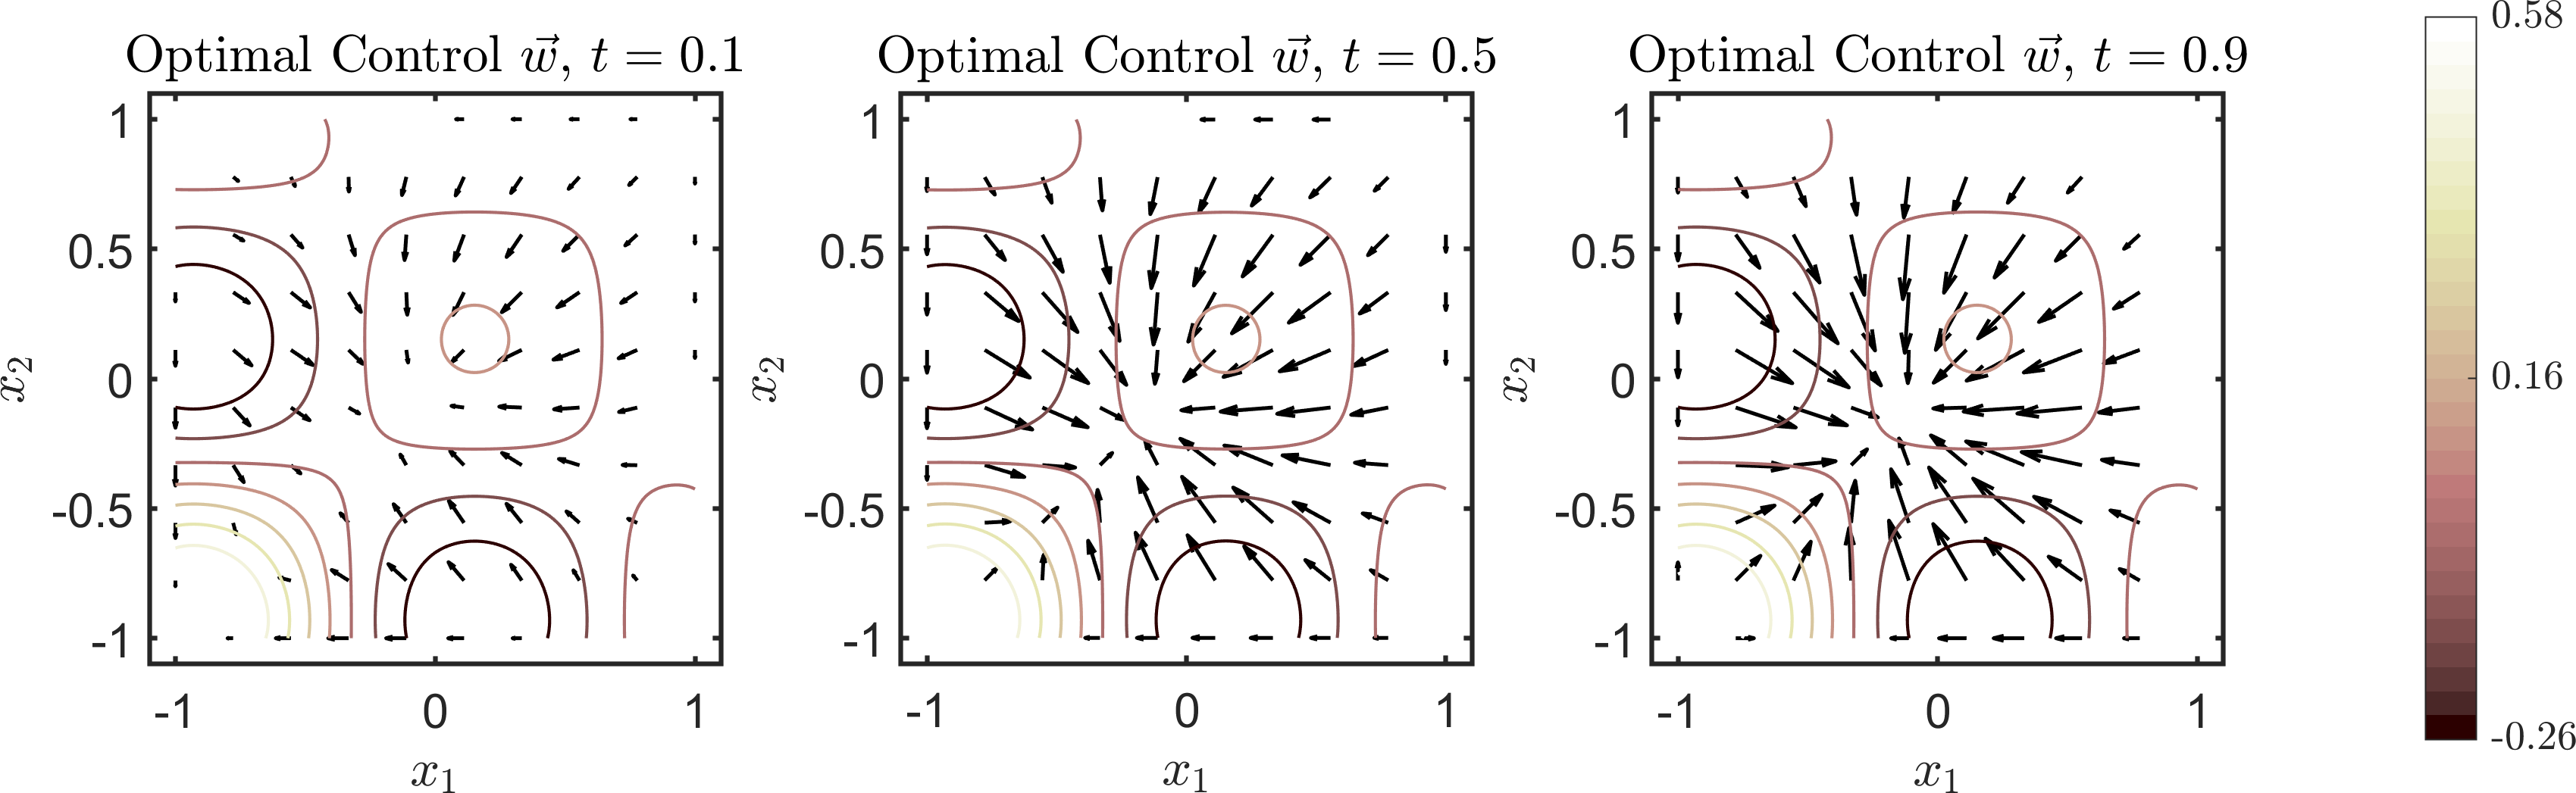
\includegraphics[scale=0.1]{FCNk1c.png}
	\caption{Neumann Flow Control: Optimal control for $\kappa = 1$ and $\beta = 10^{-3}$ and contour plot of the external potential \emph{$V_{\text{ext}}$} as before.} 
	\label{F3cc}
\end{figure}

\subsubsection{Non-linear (flow) control problem with Dirichlet boundary conditions}
The final 2D example is a flow control problem of type \eqref{AdvDiff}, with Dirichlet boundary conditions \eqref{Dirichlet}.
\begin{align*}
	\rho_0 &= \left(\frac{\pi}{4}\right)^2\cos\left(\frac{\pi x_1}{2}\right)\cos\left(\frac{\pi x_2}{2}\right) + \left(\frac{\pi}{4}\right)^2, \quad 
	V_{ext} = 2\sin\left(\frac{\pi x_1}{2}\right) \sin\left(\frac{\pi x_2}{3} - \frac{\pi}{2}\right),\\
	\hr &= (1 - t)\left(\left(\frac{\pi}{4}\right)^2\cos\left(\frac{\pi x_1}{2}\right)\cos\left(\frac{\pi x_2}{2}\right) + \left(\frac{\pi}{4}\right)^2\right) + t\left(\left(\frac{\pi}{4}\right)^2\cos\left(\frac{\pi x_1}{2}\right)\cos\left(\frac{3\pi x_2}{2}\right) + \left(\frac{\pi}{4}\right)^2\right).
\end{align*}
In this example the desired state prescribes the particles to move from one uniform bump in the middle of the domain, to accumulate in a steeper, elongated shape across the $x_1$-axis. In this example, the effect of the different interaction strengths and the external potential is clearly demonstrated, see Figure \ref{F5a}. The external potential is steep on the left side of the domain, so that most control effort is concentrated on the right side of the domain. However, for attractive particles, there also has to be more control applied in the right side of the domain, since the attractive particles work opposed to the action of spreading out along the $x_1$-axis, and the initial clump in the middle of the domain is a more natural state for this configuration, see Figure \ref{F5b}. Opposed to that is the effect that repulsive particles have on the control. In this case, most of the work of the control is done to push the particles together, see Figure \ref{F5c}. The controls can be seen in Figures \ref{F5ac}, \ref{F5bc} and \ref{F5cc}.
The results can be seen in Table \ref{TabFCD}.


\begin{table}
\centering
\begin{tabular}{ | c | c || c | c | c | c | c ||}
\hline
\multicolumn{2}{|c||}{}& $\beta = 10^{-5}$ & $\beta = 10^{-3}$ & $\beta = 10^{-1}$ & $\beta = 10^{1}$ & $\beta = 10^{3}$  \\
\hline
\hline
\multirow{2}{*}{$\kappa= \numprint{0}$}  & $\mathcal{J}_{uc}$ & $\numprint{0.1585}$ & $\numprint{0.1585}$ & $\numprint{0.1585}$ & $\numprint{0.1585}$ & $\numprint{0.1585}$\\
 & $\mathcal{J}_c$ & $\numprint{0.0004}$ & $\numprint{0.0077}$ & $\numprint{0.1302}$ & $\numprint{0.1582}$ & $\numprint{0.1585}$\\
\hline
\multirow{2}{*}{$\kappa= \numprint{1}$}  & $\mathcal{J}_{uc}$ & $\numprint{0.2124}$ & $\numprint{0.2124}$ & $\numprint{0.2124}$ & $\numprint{0.2124}$ & $\numprint{0.2124}$\\
 & $\mathcal{J}_c$ & $\numprint{0.0004}$ & $\numprint{0.0103}$ & $\numprint{0.1852}$ & $\numprint{0.2121}$ & $\numprint{0.2124}$\\
\hline
\multirow{2}{*}{$\kappa= \numprint{-1}$}  & $\mathcal{J}_{uc}$ & $\numprint{0.4031}$ & $\numprint{0.4031}$ & $\numprint{0.4031}$ & $\numprint{0.4031}$ & $\numprint{0.4031}$\\
 & $\mathcal{J}_c$ & $\numprint{0.0005}$ & $\numprint{0.0086}$ & $\numprint{0.1739}$ & $\numprint{0.3867}$ & $\numprint{0.4029}$\\
\hline
\end{tabular}
\caption{Flow Control Dirichlet Problem: Cost when $w=0$ and optimal control cost for a range of $\kappa$, $\beta$. For $\beta = 10$, the cost functionals differ by $10^-4$ for $\kappa = 0$ and $\kappa = 1$ and by $10^-2$ for $\kappa = -1$. For $\beta = 10^3$, the cost functionals differ by $10^{-7}$ for $\kappa = 0$, by $10^{-6}$ for $\kappa = 1$, and by $10^{-4}$ for $\kappa = -1$.}
\label{TabFCD}
\end{table}

\begin{figure}[h]
	\centering
	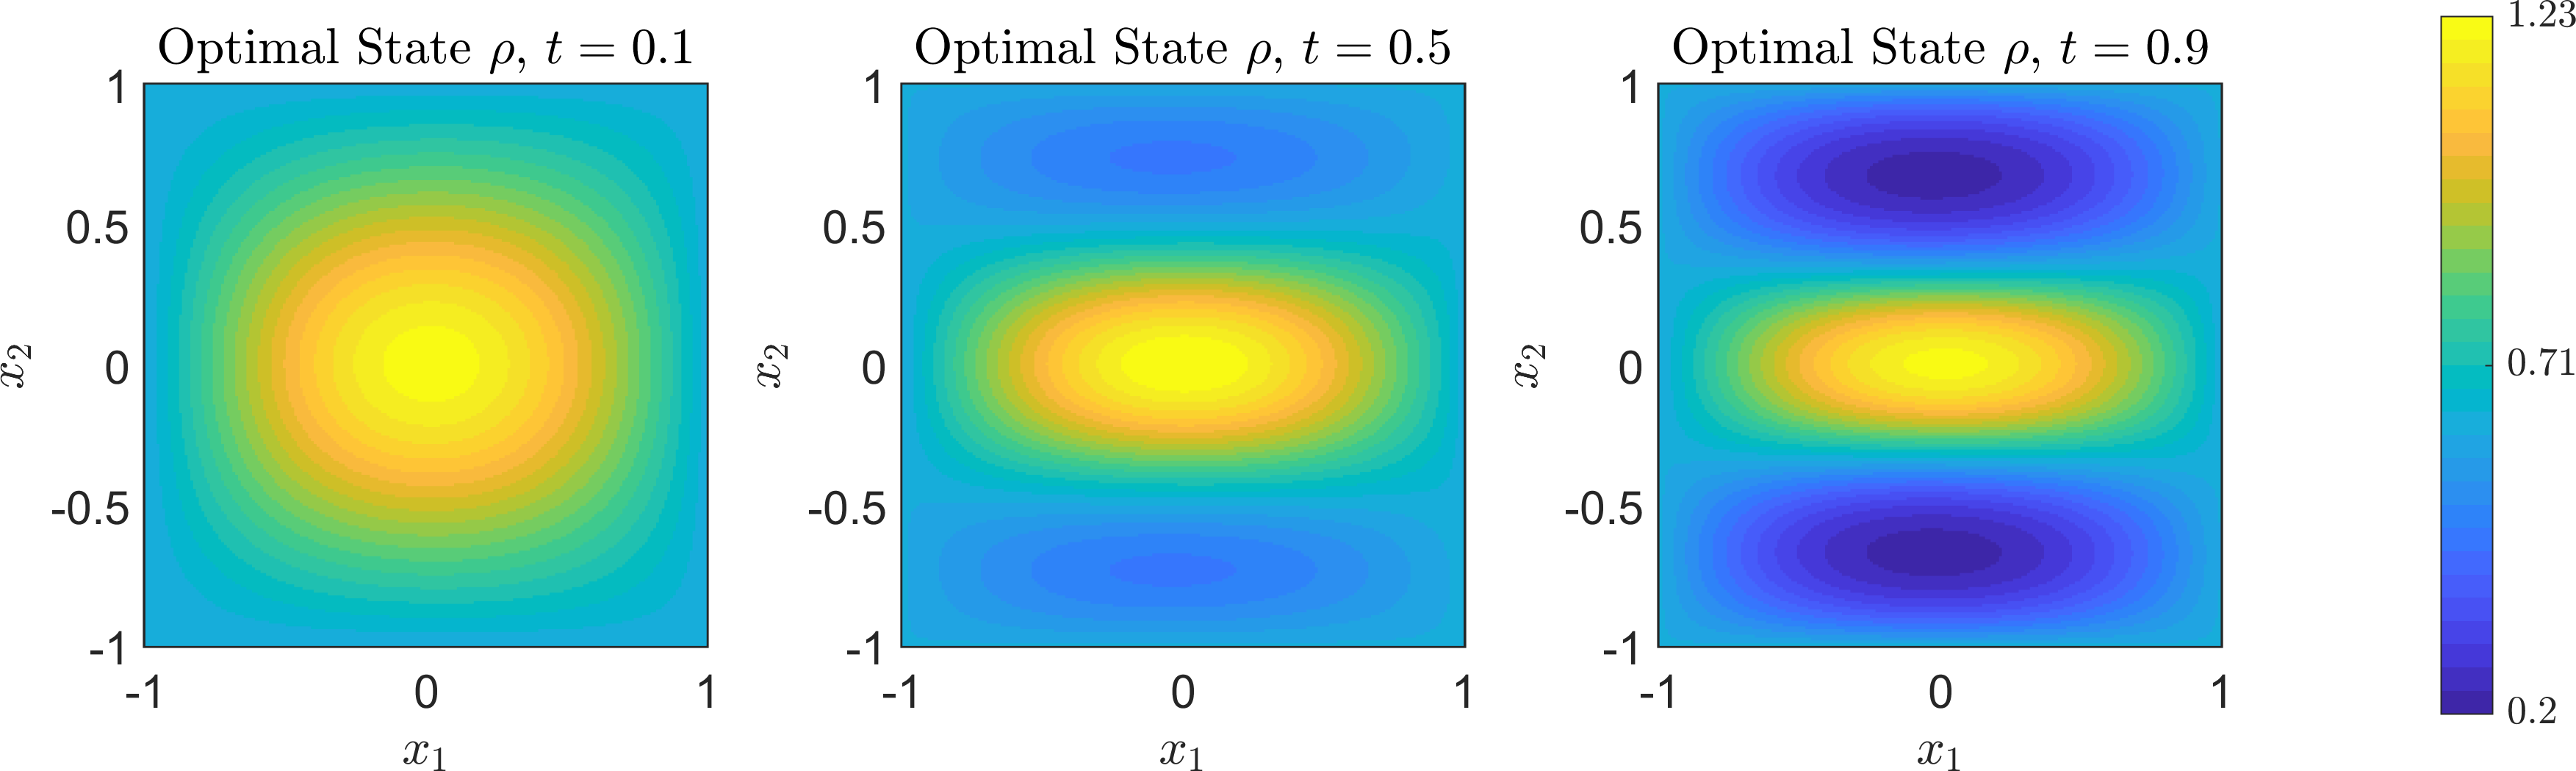
\includegraphics[scale=0.1]{FCDk0.png}
	\caption{Dirichlet Flow Control: Optimal $\rho$ for $\kappa = 0$ and $\beta = 10^{-3}$.} 
	\label{F5a}
\end{figure}
\begin{figure}[h]
	\centering
	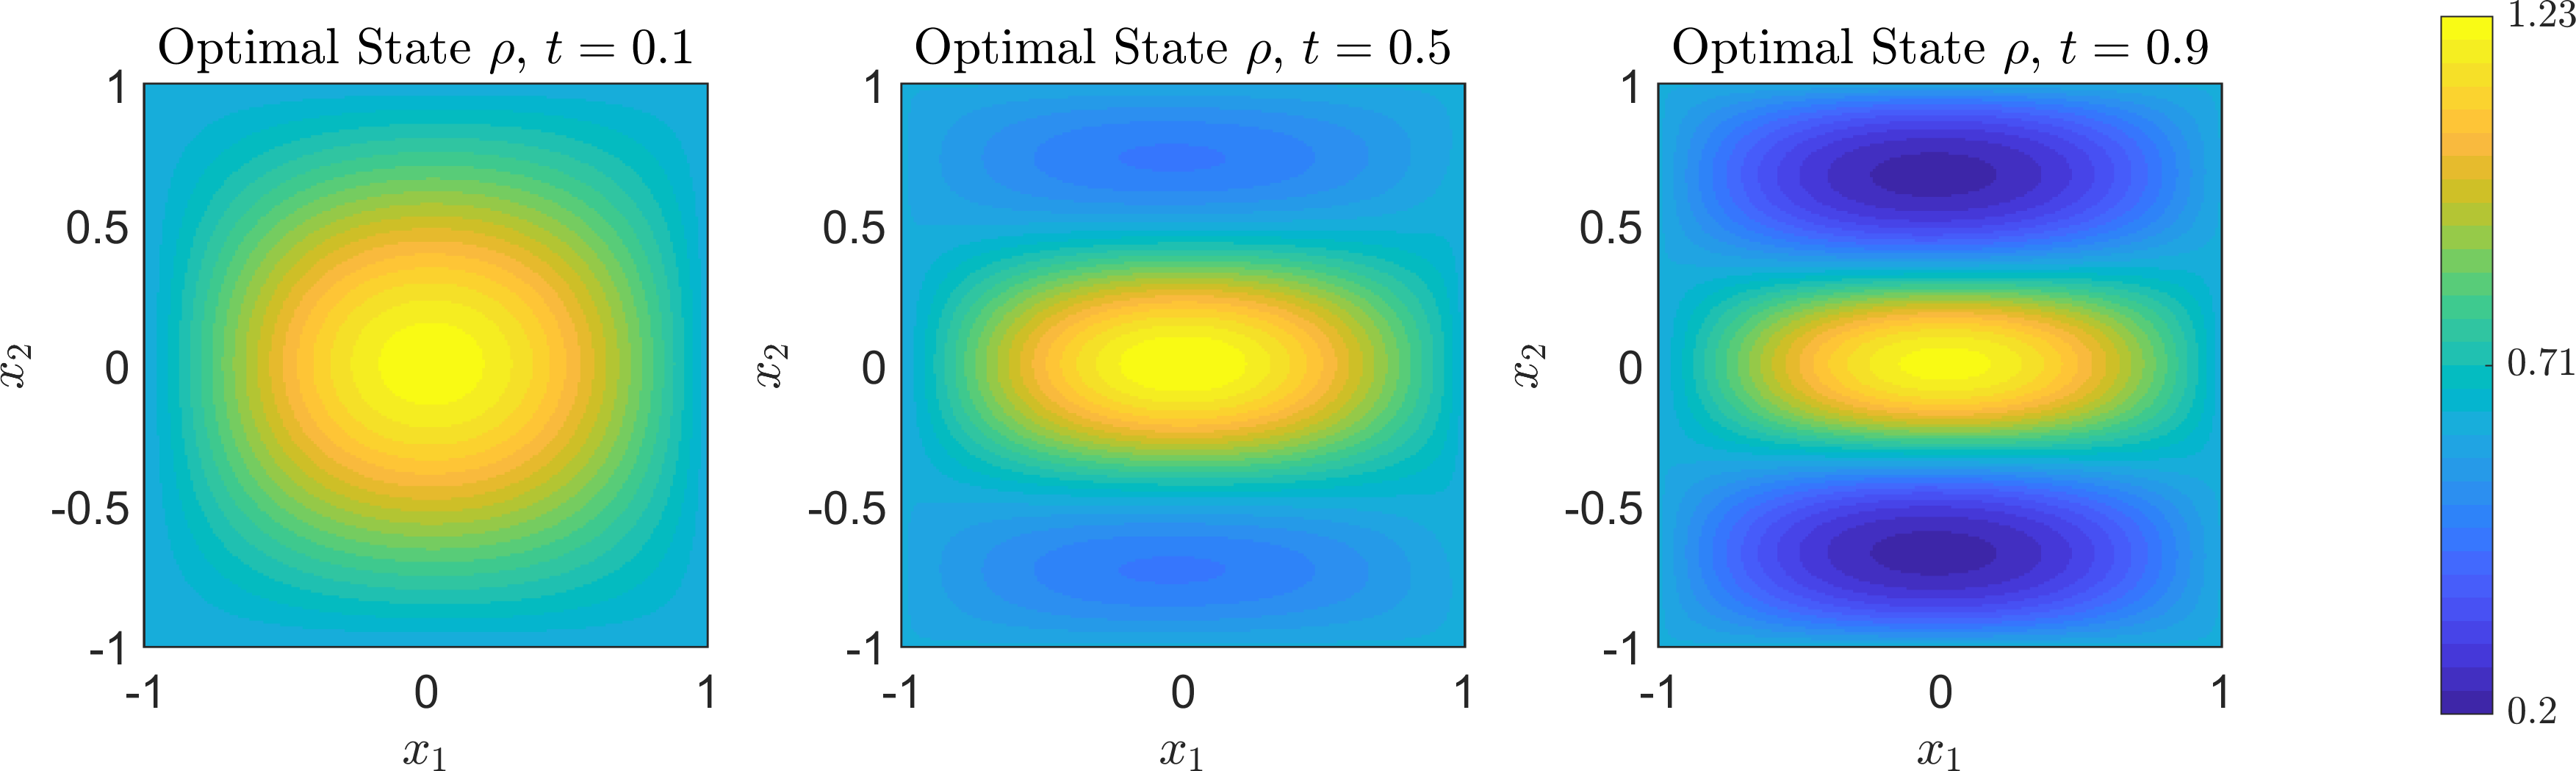
\includegraphics[scale=0.1]{FCDkn1.png}
	\caption{Dirichlet Flow Control: Optimal $\rho$ for $\kappa = -1$ and $\beta = 10^{-3}$.} 
	\label{F5b}
\end{figure}
\begin{figure}[h]
	\centering
	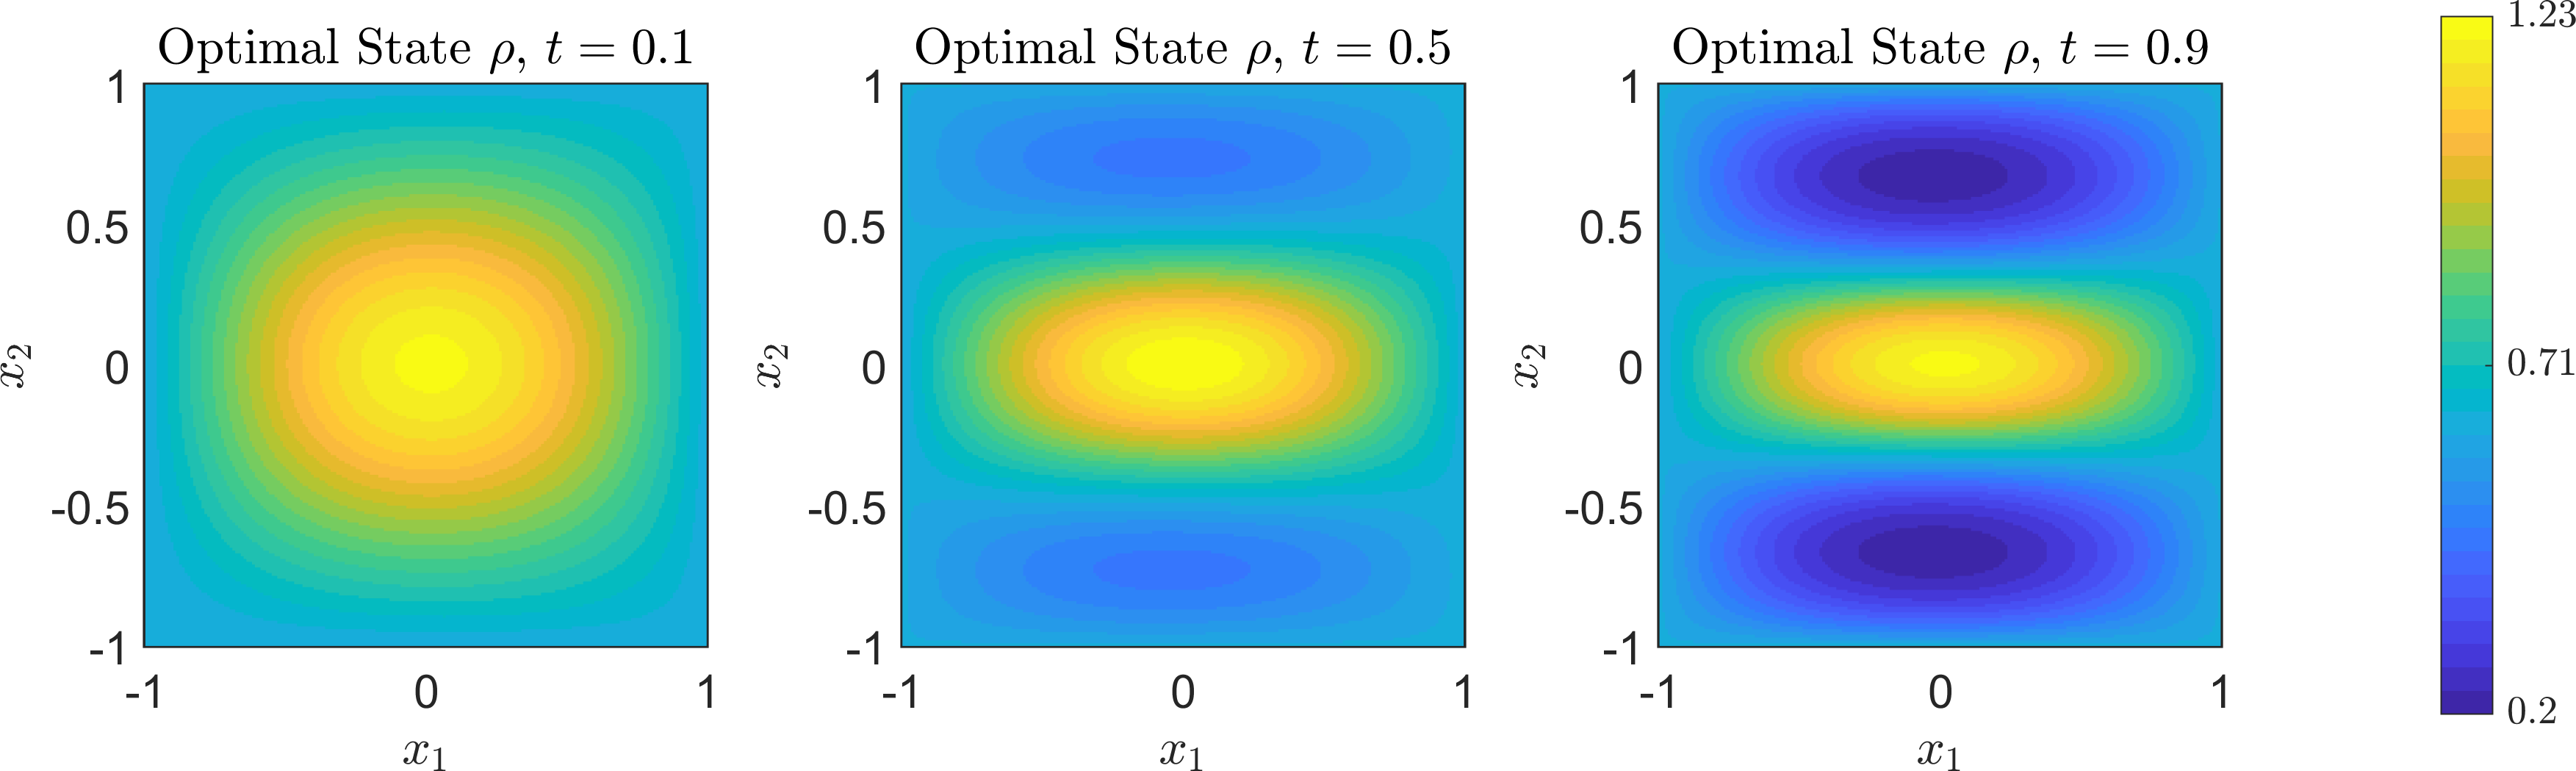
\includegraphics[scale=0.1]{FCDk1.png}
	\caption{Dirichlet Flow Control: Optimal $\rho$ for $\kappa = 1$ and $\beta = 10^{-3}$.} 
	\label{F5c}
\end{figure}



\begin{figure}[h]
	\centering
	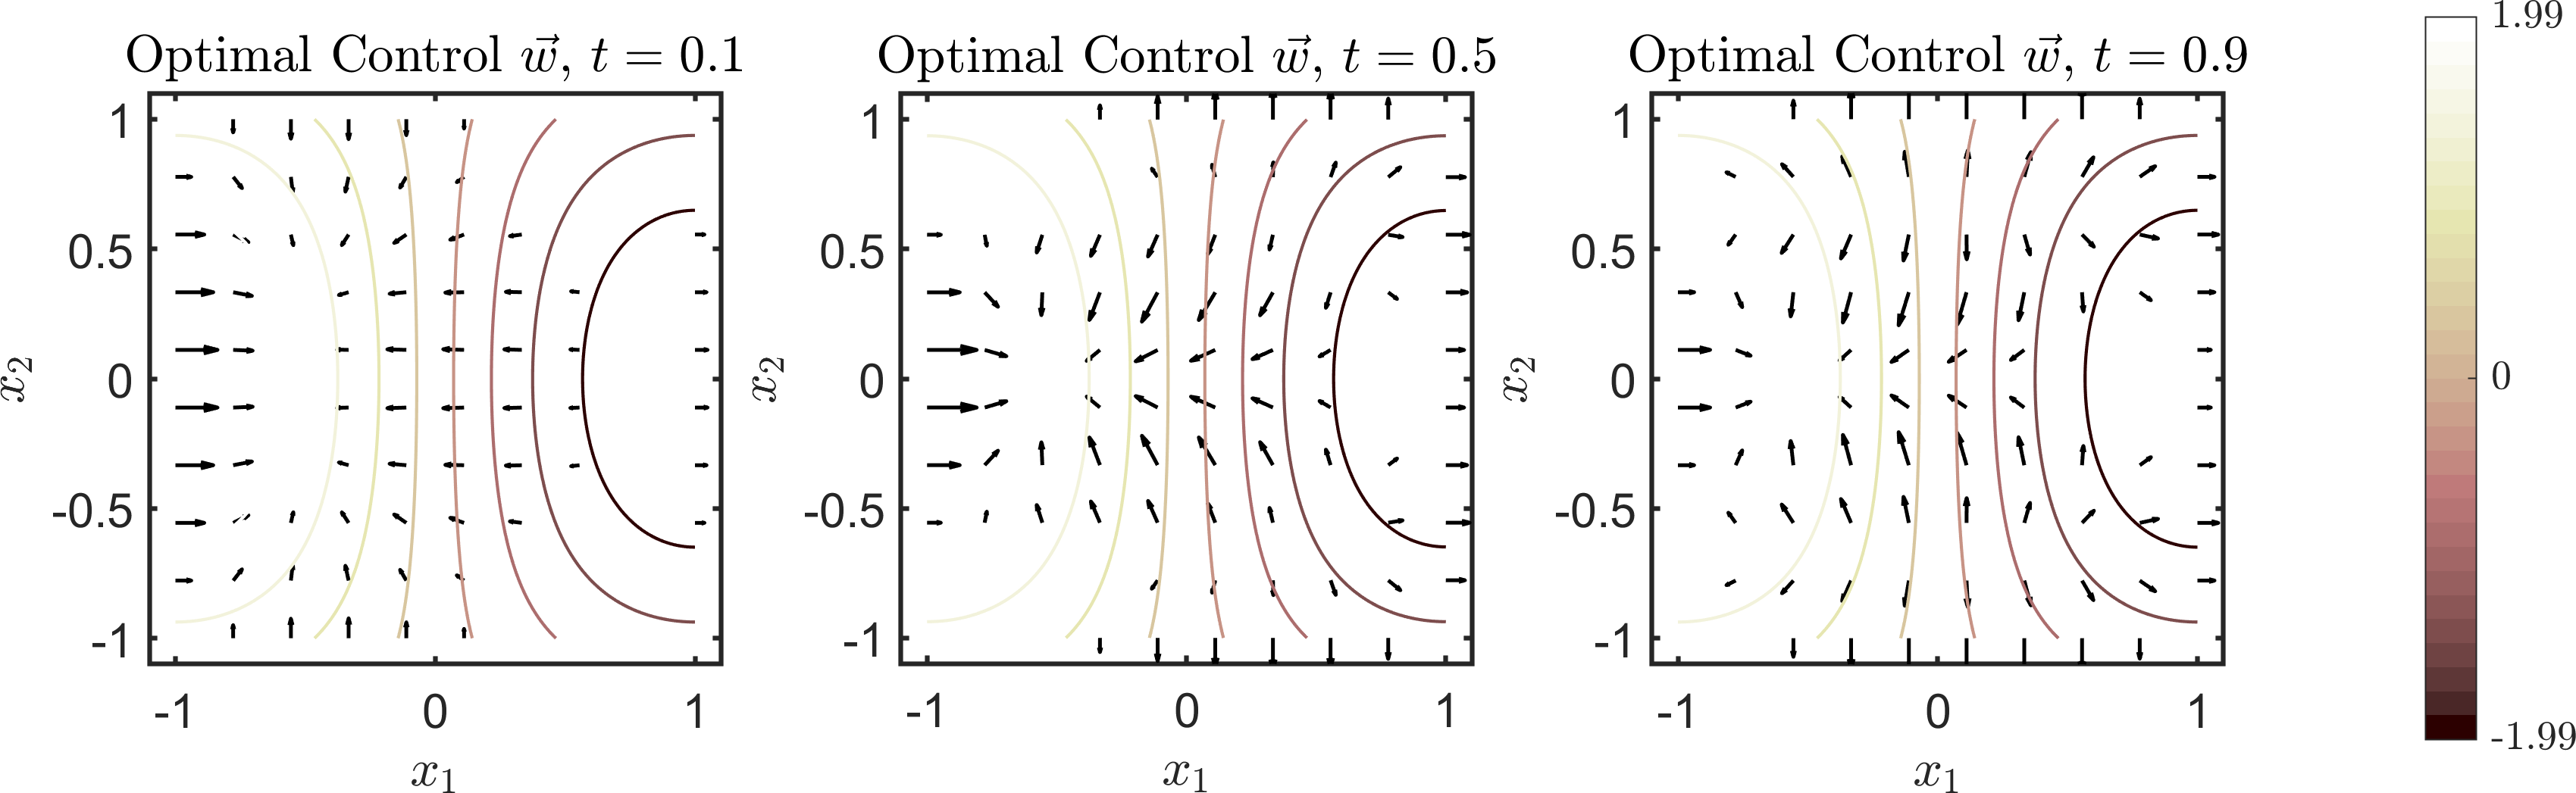
\includegraphics[scale=0.1]{FCDk0c.png}
	\caption{Dirichlet Flow Control: Optimal control for $\kappa = 0$ and $\beta = 10^{-3}$. A contour plot of the external potential \emph{$V_{\text{ext}}$} is superimposed on the control plots for reference, with a corresponding colorbar on the left-hand side.} 
	\label{F5ac}
\end{figure}
\begin{figure}[h]
	\centering
	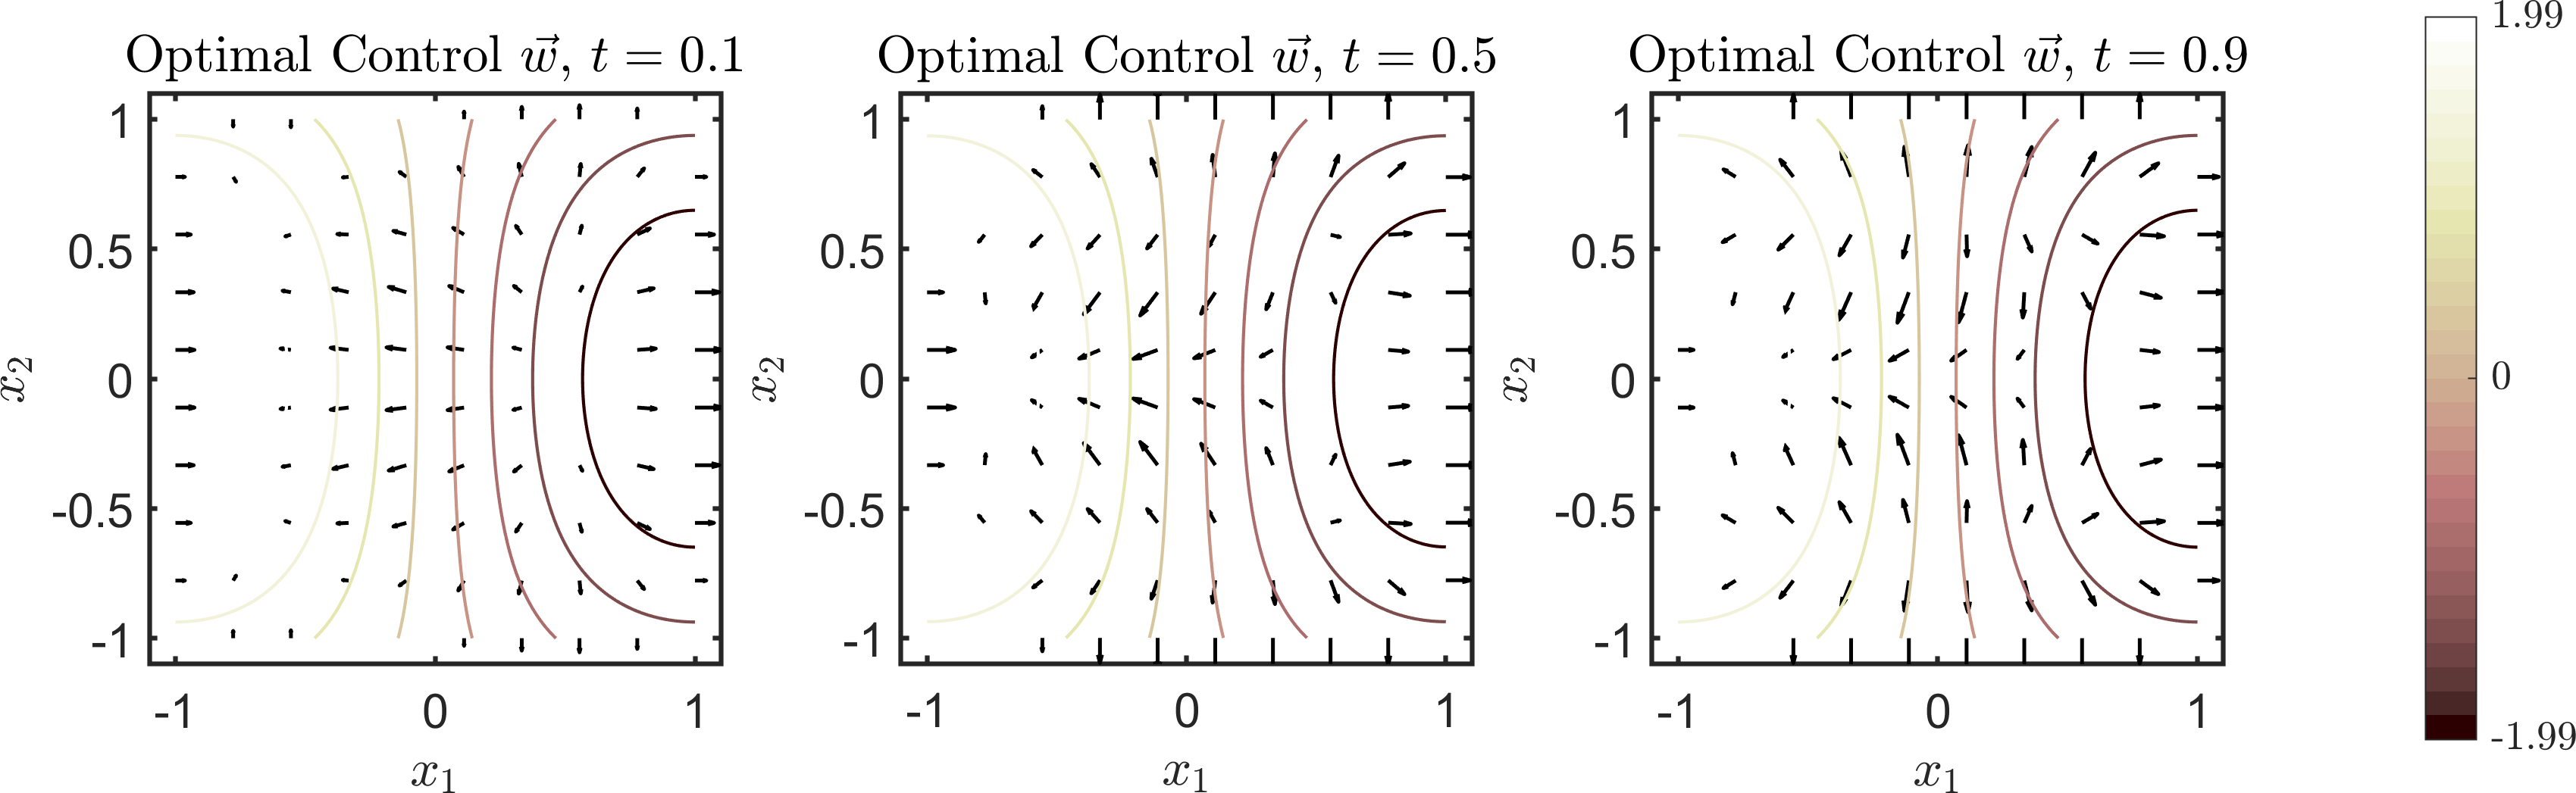
\includegraphics[scale=0.1]{FCDkn1c.png}
	\caption{Dirichlet Flow Control: Optimal control for $\kappa = -1$ and $\beta = 10^{-3}$ and contour plot of the external potential \emph{$V_{\text{ext}}$} as before.} 
	\label{F5bc}
\end{figure}
\begin{figure}[h]
	\centering
	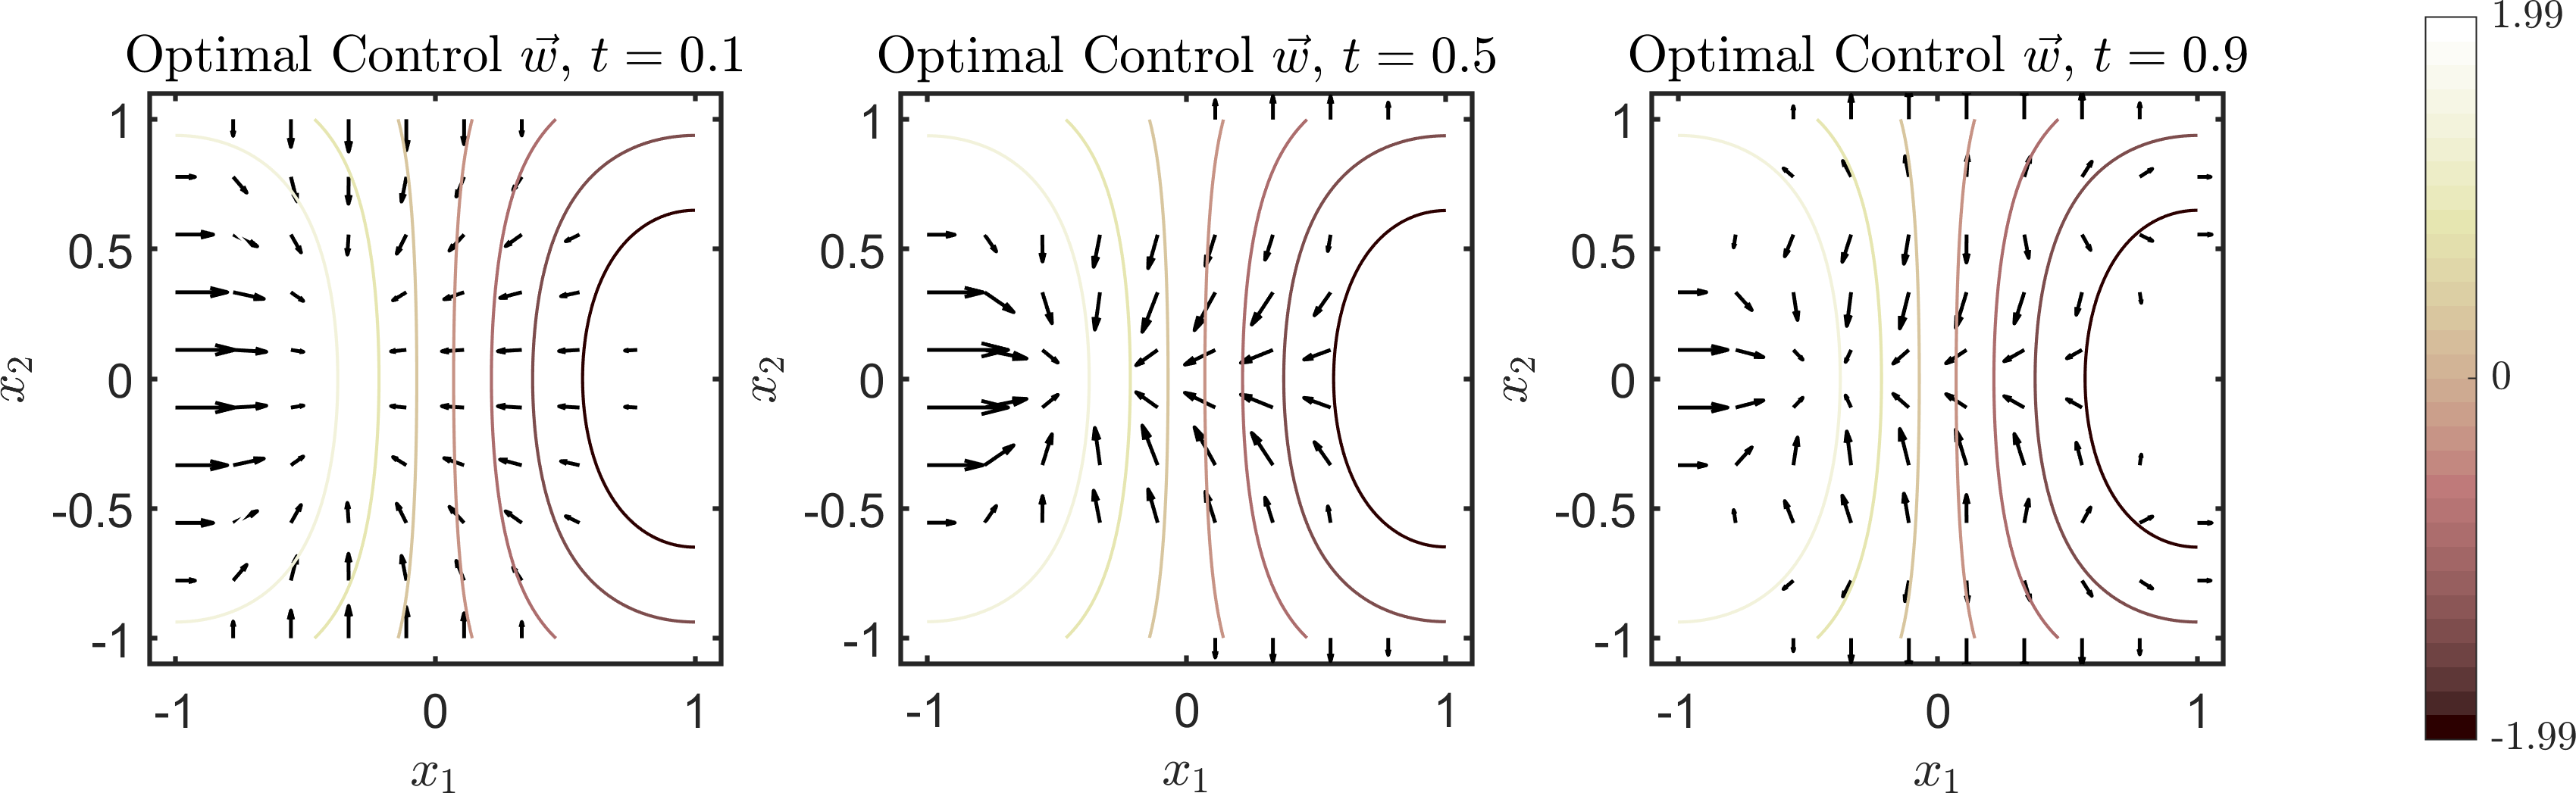
\includegraphics[scale=0.1]{FCDk1c.png}
	\caption{Dirichlet Flow Control: Optimal control for $\kappa = 1$ and $\beta = 10^{-3}$ and contour plot of the external potential \emph{$V_{\text{ext}}$} as before.} 
	\label{F5cc}
\end{figure}

\subsection{Three-dimensional Example}
We consider a three-dimensional example featuring the non-linear flow control problem \eqref{AdvDiff} with boundary conditions \eqref{NoFlux}, since this is the most challenging combination of control type and boundary conditions.
The chosen inputs for this example are:
\begin{align*}
	\rho_0 &= \frac{1}{8}, \quad \hr = \frac{1}{8}(1-t) + t\left(\frac{\pi}{4}\right)^3\cos\left(\frac{\pi x_1}{2}\right)\cos\left(\frac{\pi x_2}{2}\right)\cos\left(\frac{\pi x_3}{2}\right),\\
	V_{ext} &= \left(\left(x_1 + 0.3\right)^2 - 1\right)\left(\left(x_1 - 0.4\right)^2 - 0.5\right) \left(\left(x_2 + 0.3\right)^2 - 1\right)\left(\left(x_2 - 0.4\right)^2 - 0.5\right)\\
	&\ \quad\left(\left(x_3 + 0.3\right)^2 - 1\right)\left(\left(x_3 - 0.4\right)^2 - 0.5\right).
\end{align*}
The effect of the different interaction strengths is clearly displayed in Figures \ref{F2}, \ref{F3} and \ref{F4} and is particularly obvious in earlier times of the particle evolution.
The imposed external potential is shown in Figure \ref{F1}.
In Figures \ref{F5}, \ref{F6} and \ref{F7}, the controls for different interaction strengths are shown. It is evident, that attractive particles support the control to push the particles into a cluster in the middle of the domain, as prescribed by the desired state $\hr$, while more control is needed for a similar effect in the repulsive setup.
This example is only run for $\beta = 10^{-3}$, due to a running time of approximately $35$ hours per problem. We get for $\kappa = 0$, $\mathcal J_c = 0.0078$. This can be compared to $\mathcal J_{uc} = 0.0195$ from the computed forward problem with $\w = \vec 0$. For $\kappa = 1$, we get that $\mathcal J_c = 0.0102$ as opposed to $\mathcal J_{uc} = 0.0232$ in the uncontrolled case and for $\kappa = -1$ we have $\mathcal J_c = 0.0059$, which is compared to the uncontrolled value $\mathcal J_{uc} = 0.0477$.


	\begin{figure}[h]
		\centering
		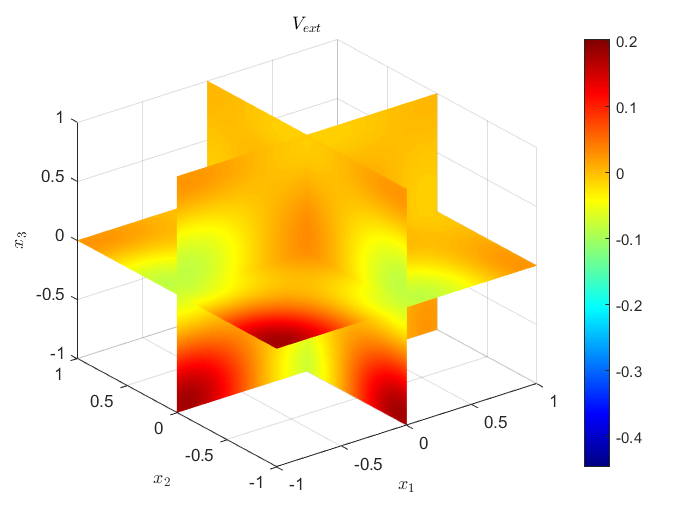
\includegraphics[scale=0.7]{Vext3D.png}
		\caption{External Potential $V_{ext}$} 
		\label{F1}
	\end{figure}

	

\begin{figure}[h]
	\centering
	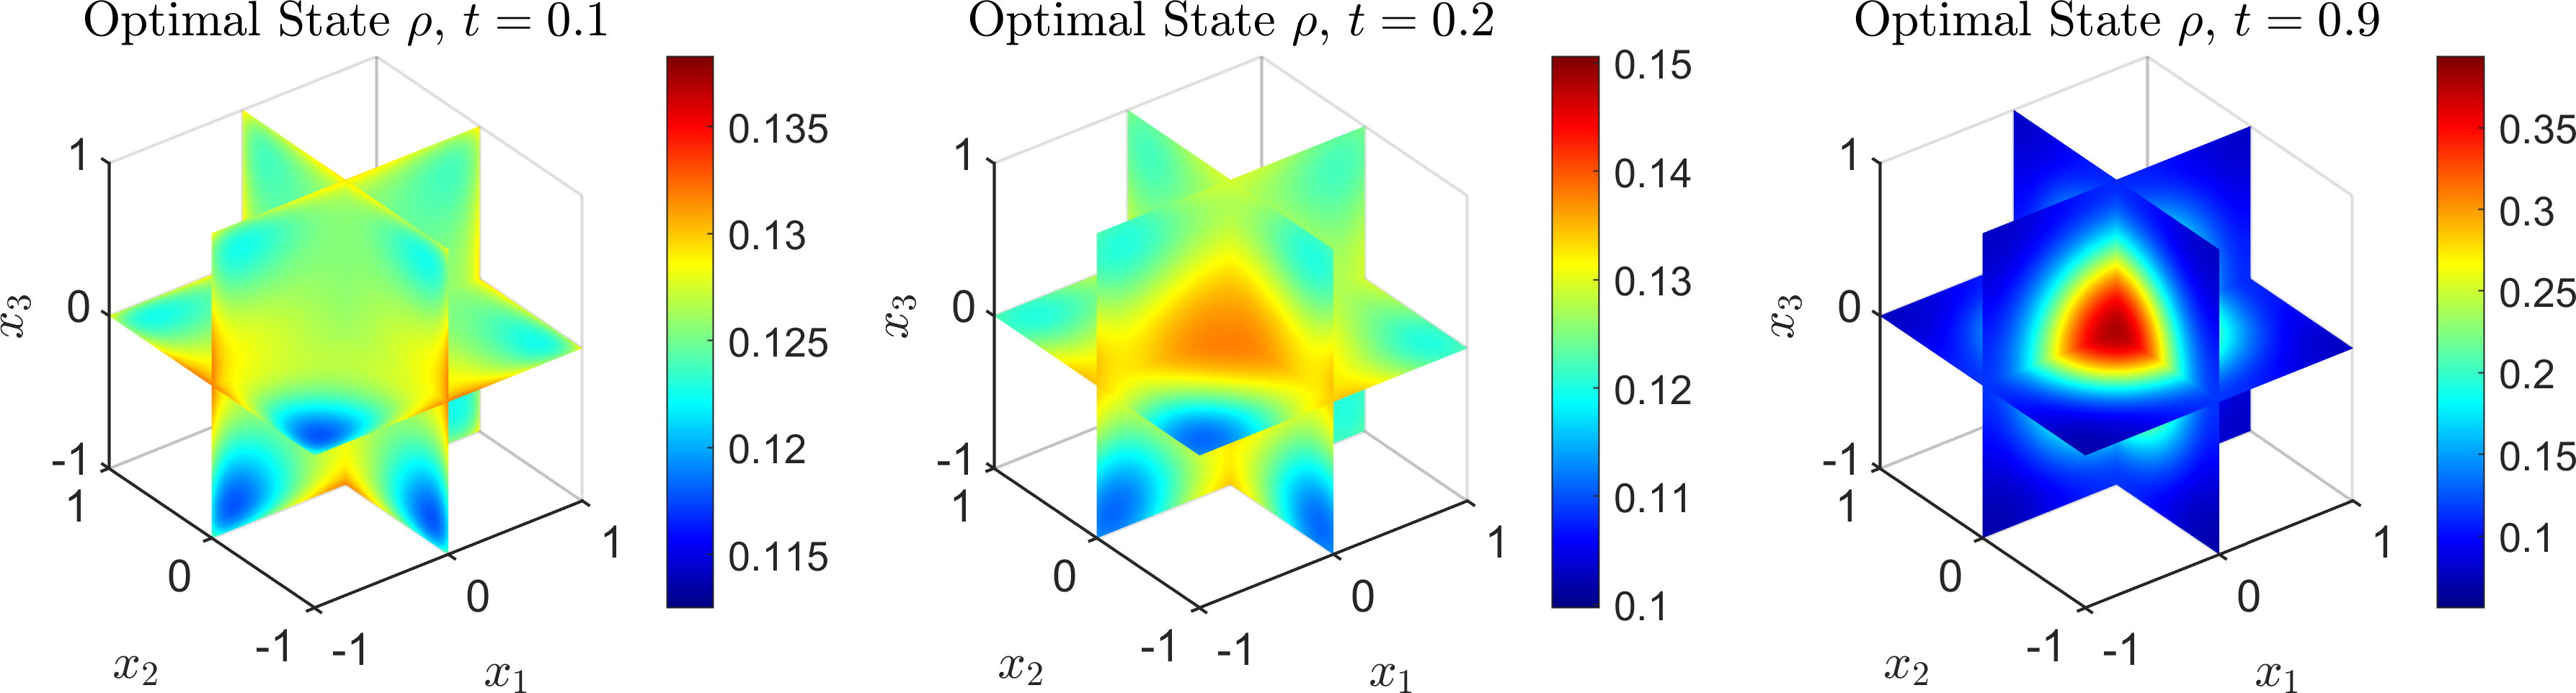
\includegraphics[scale=0.1]{rhok1.png}
	\caption{Optimal state $\rho$ for $\kappa = 1$.} 
	\label{F2}
\end{figure}
\begin{figure}[h]
	\centering
	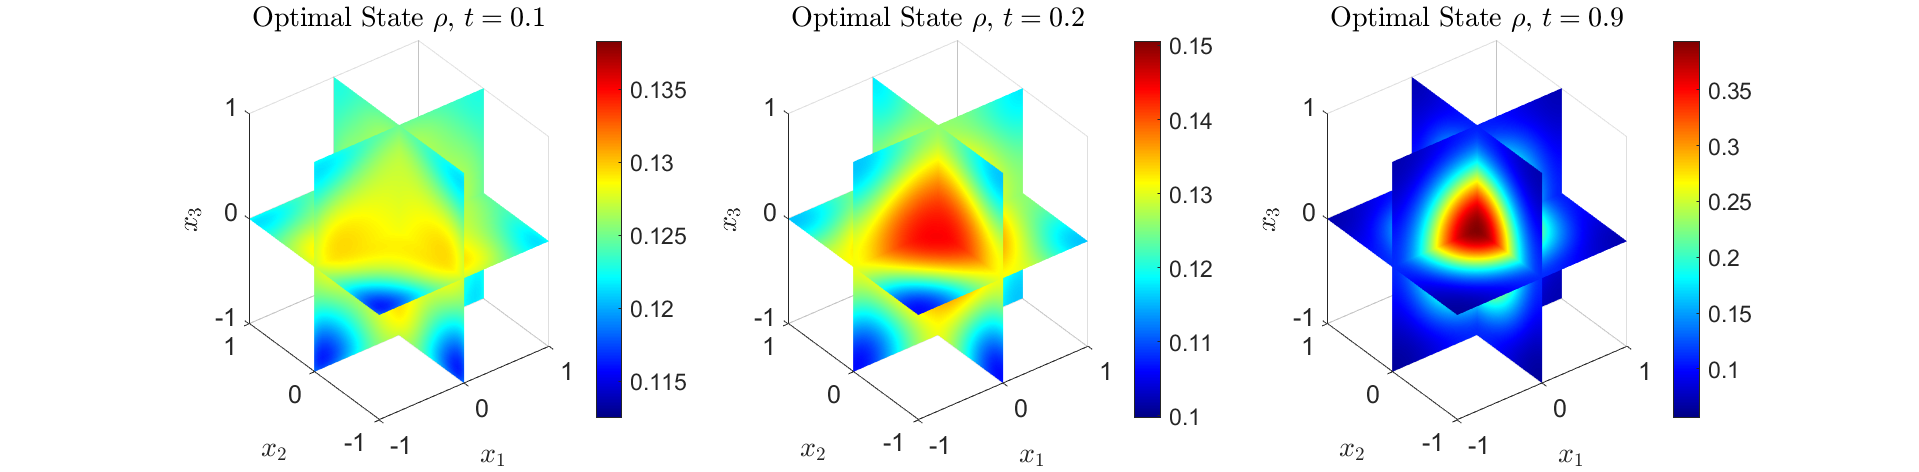
\includegraphics[scale=0.1]{rhok0.png}
	\caption{Optimal state $\rho$ for $\kappa = 0$.} 
	\label{F3}
\end{figure}
\begin{figure}[h]
	\centering
	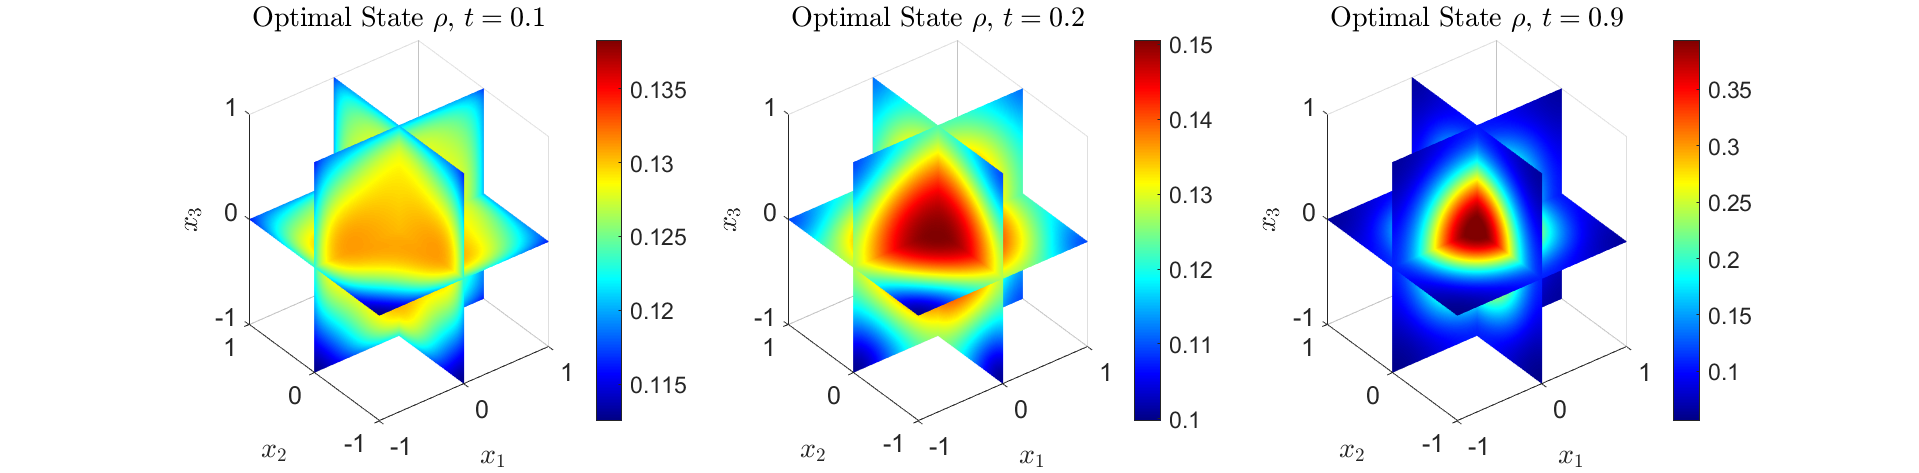
\includegraphics[scale=0.1]{rhokn1.png}
	\caption{Optimal state $\rho$ for $\kappa = -1$.} 
	\label{F4}
\end{figure}
%	
\begin{figure}[h]
	\centering
	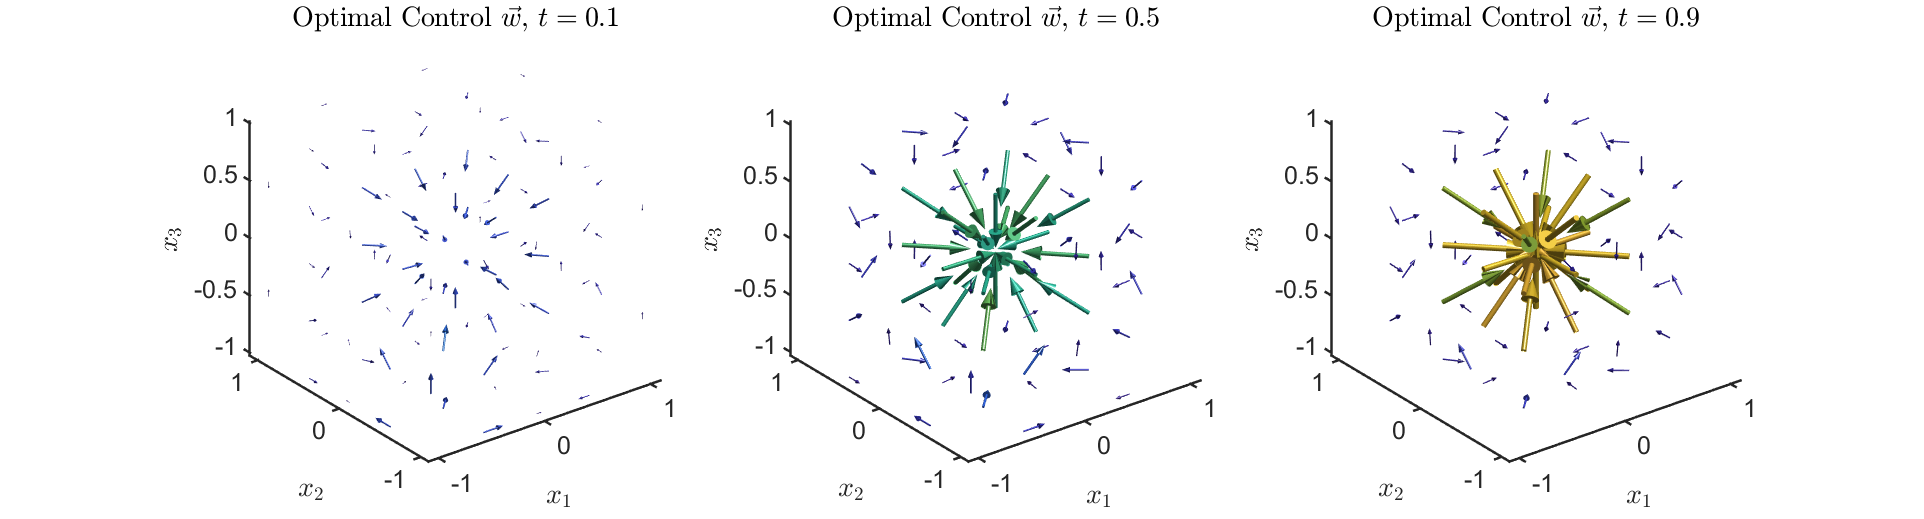
\includegraphics[scale=0.1]{Controlk1.png}
	\caption{Optimal control $\w$ for $\kappa = 1$.} 
	\label{F5}
\end{figure}
\begin{figure}[h]
	\centering
	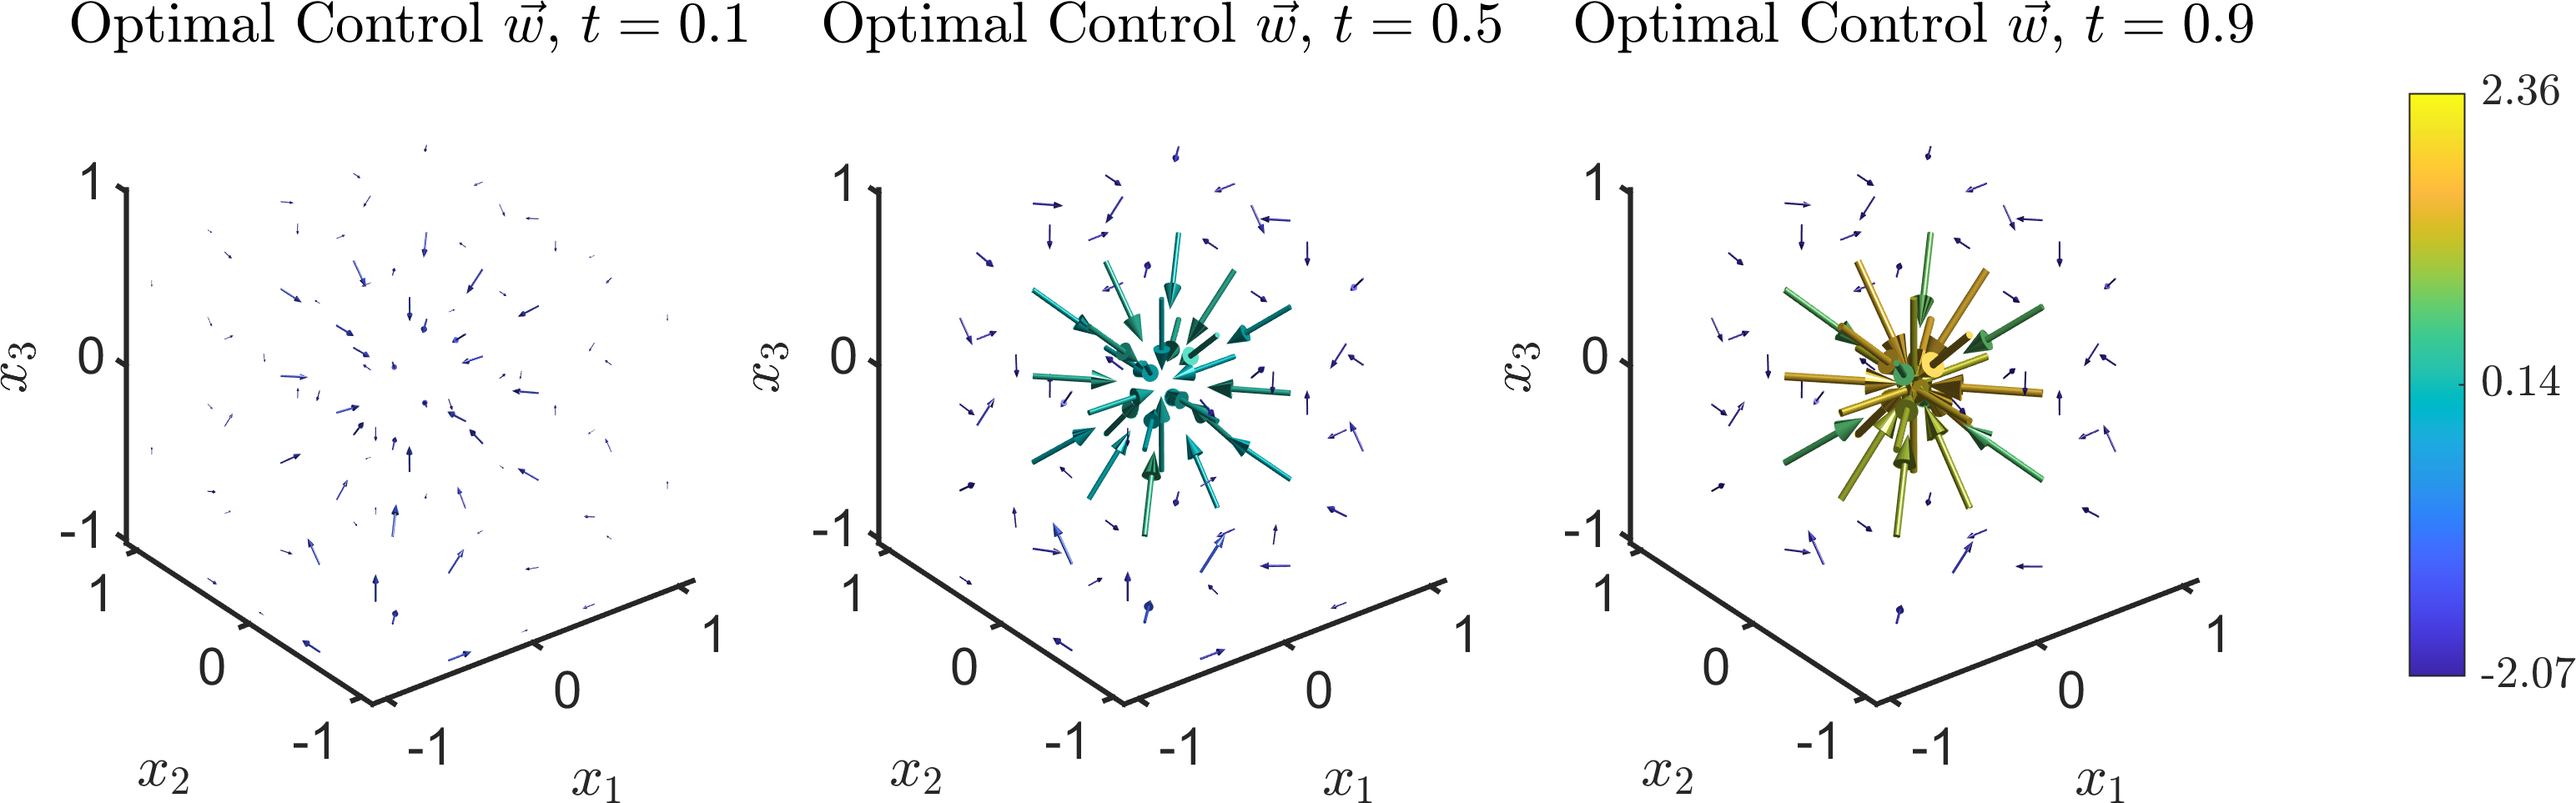
\includegraphics[scale=0.1]{Controlk0.png}
	\caption{Optimal control $\w$ for $\kappa = 0$.} 
	\label{F6}
\end{figure}
\begin{figure}[h]
	\centering
	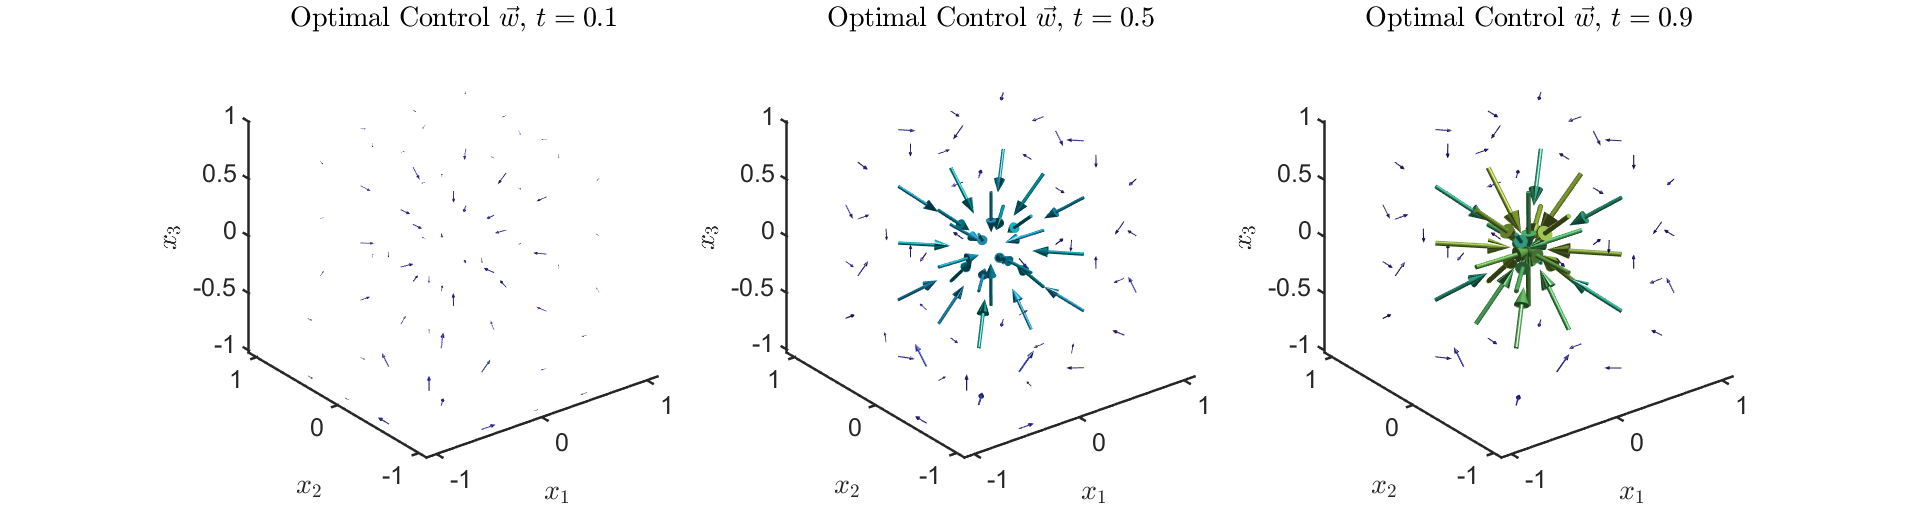
\includegraphics[scale=0.1]{Controlkn1.png}
	\caption{Optimal control $\w$ for $\kappa = -1$.} 
	\label{F7}
\end{figure}

Figures \ref{Con1}, \ref{Con2}, \ref{Con3} and \ref{Con4} show the convergence of the Newton-Krylov method for different $\beta$ for each 2D problem considered above.

\begin{figure}[h]
	\centering
	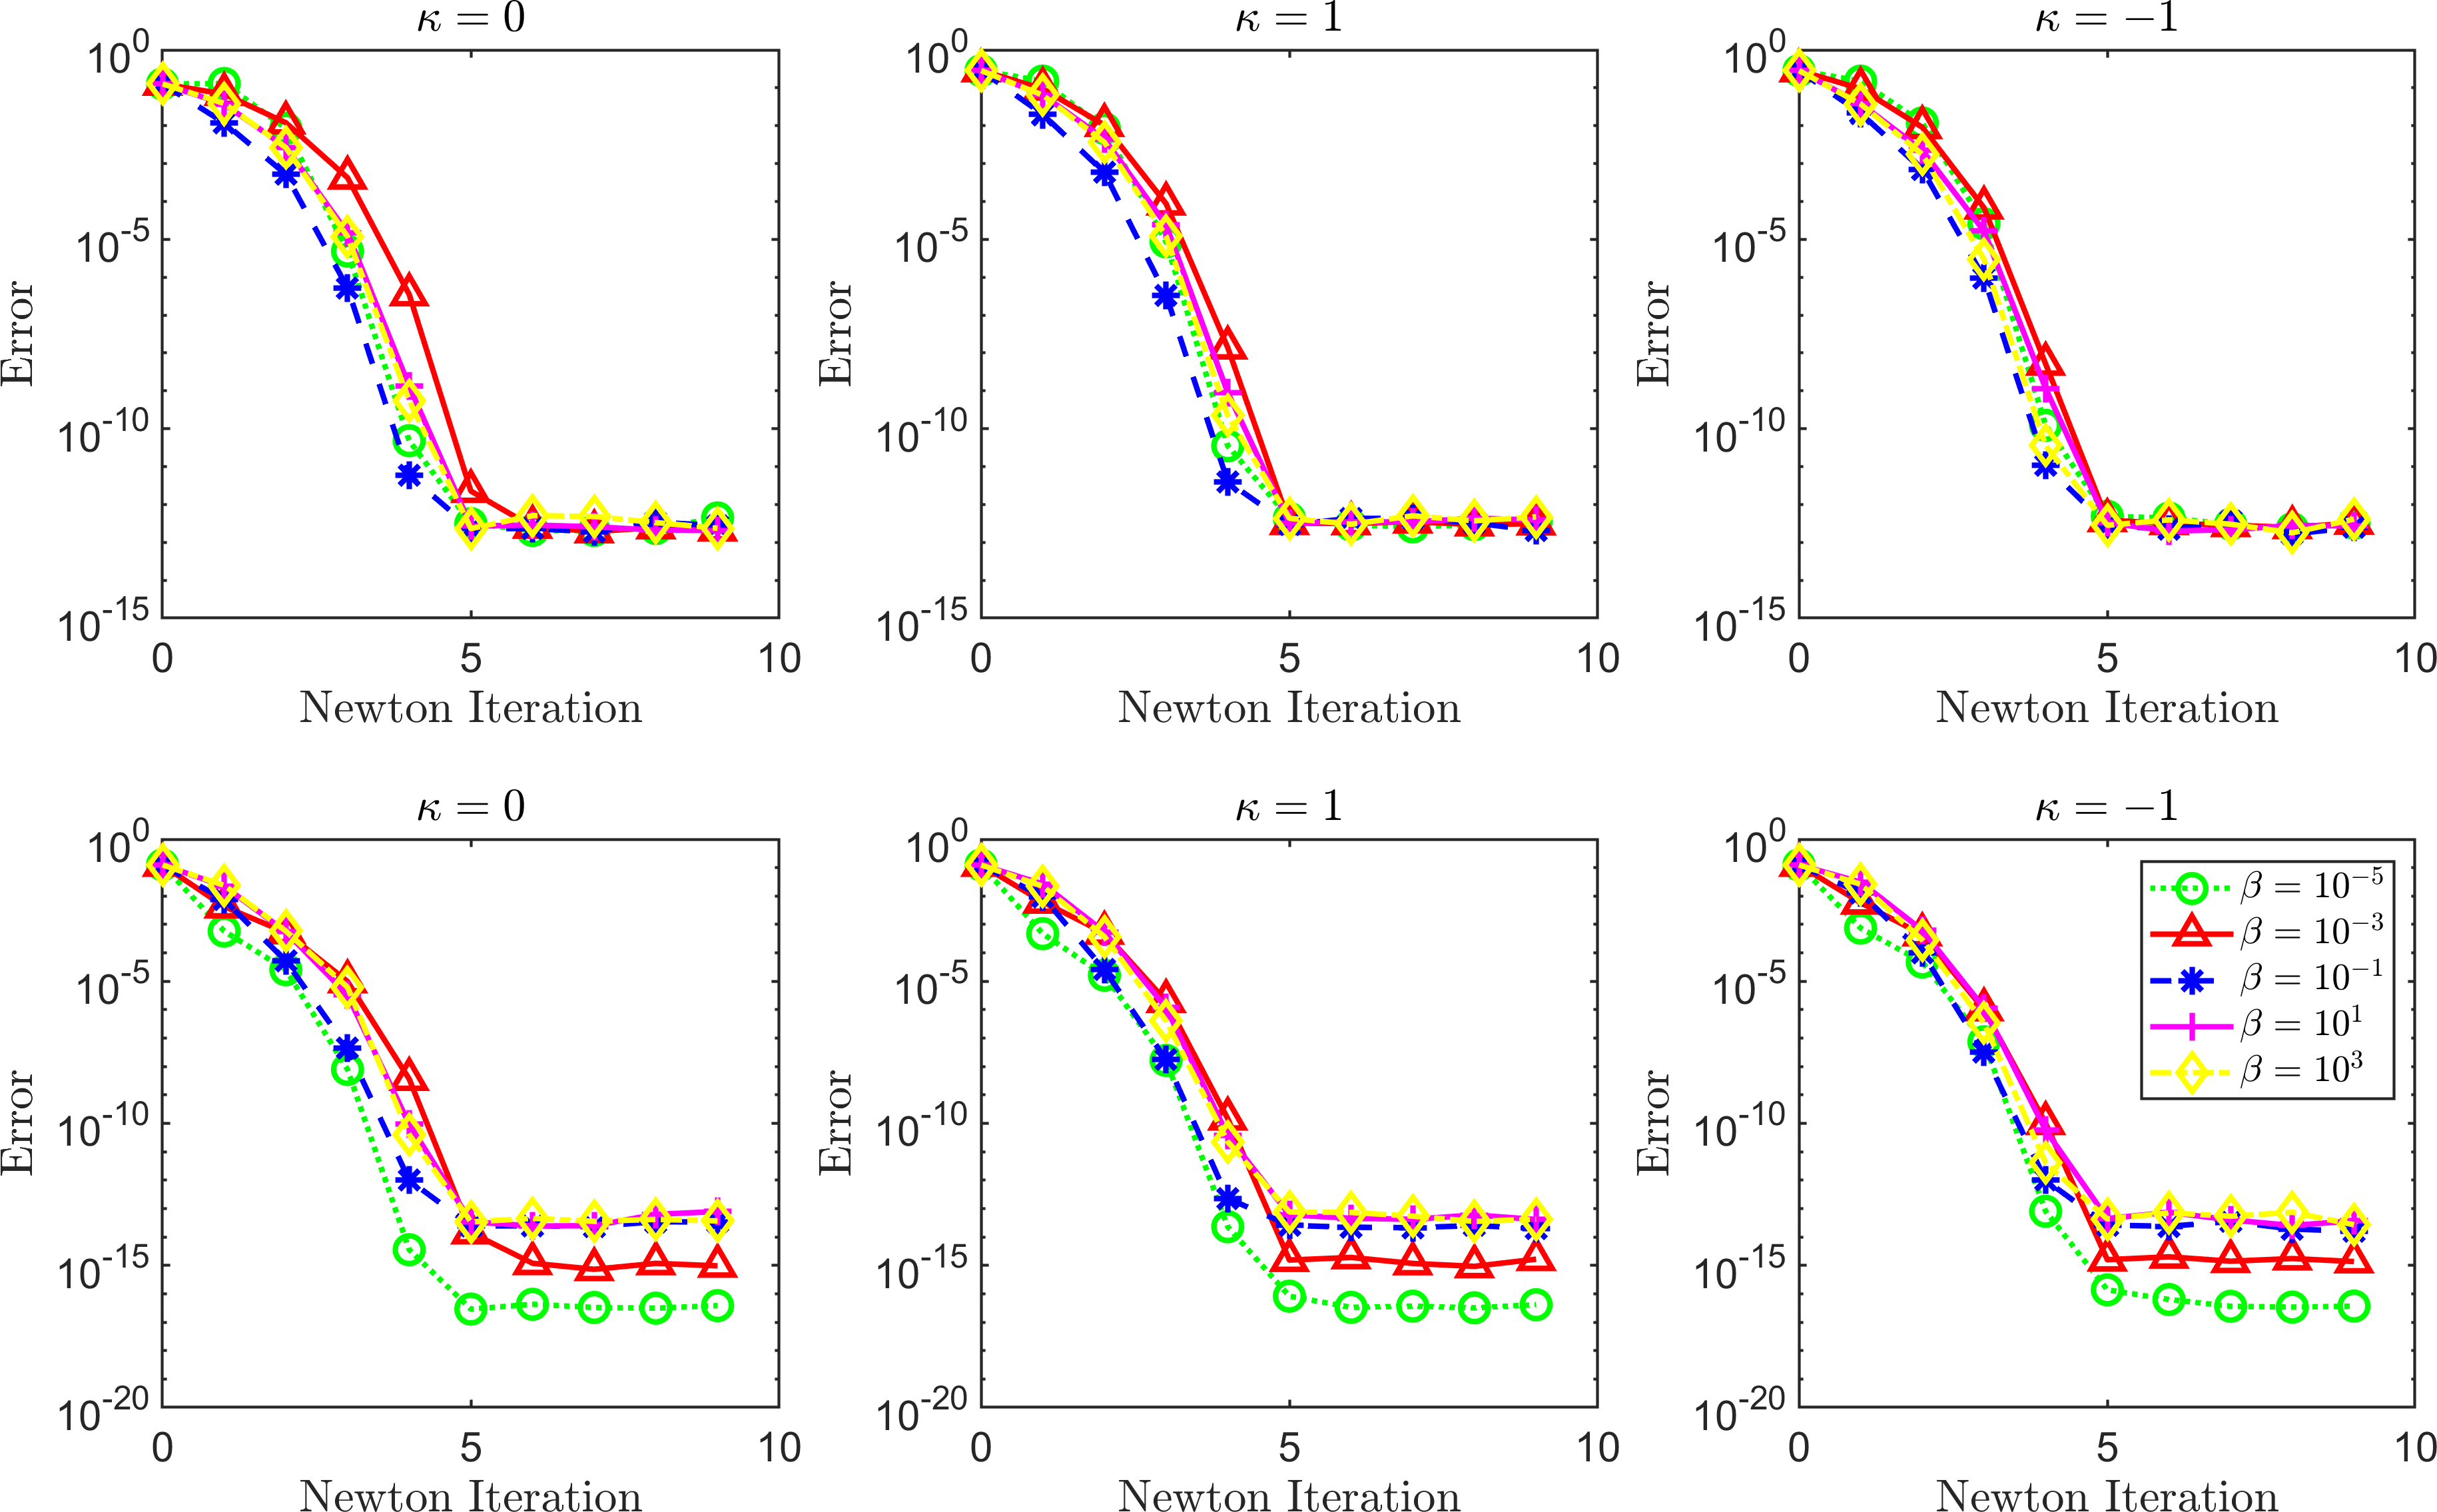
\includegraphics[scale=0.1]{SCNConvergence.png}
	\caption{Convergence of the Newton-Krylov Algorithm for no-flux source control. Top three plots show the convergence in the state variable for different $\kappa$, while the bottom plots show the convergence in the adjoint variable.} 
	\label{Con1}
\end{figure}
\begin{figure}[h]
	\centering
	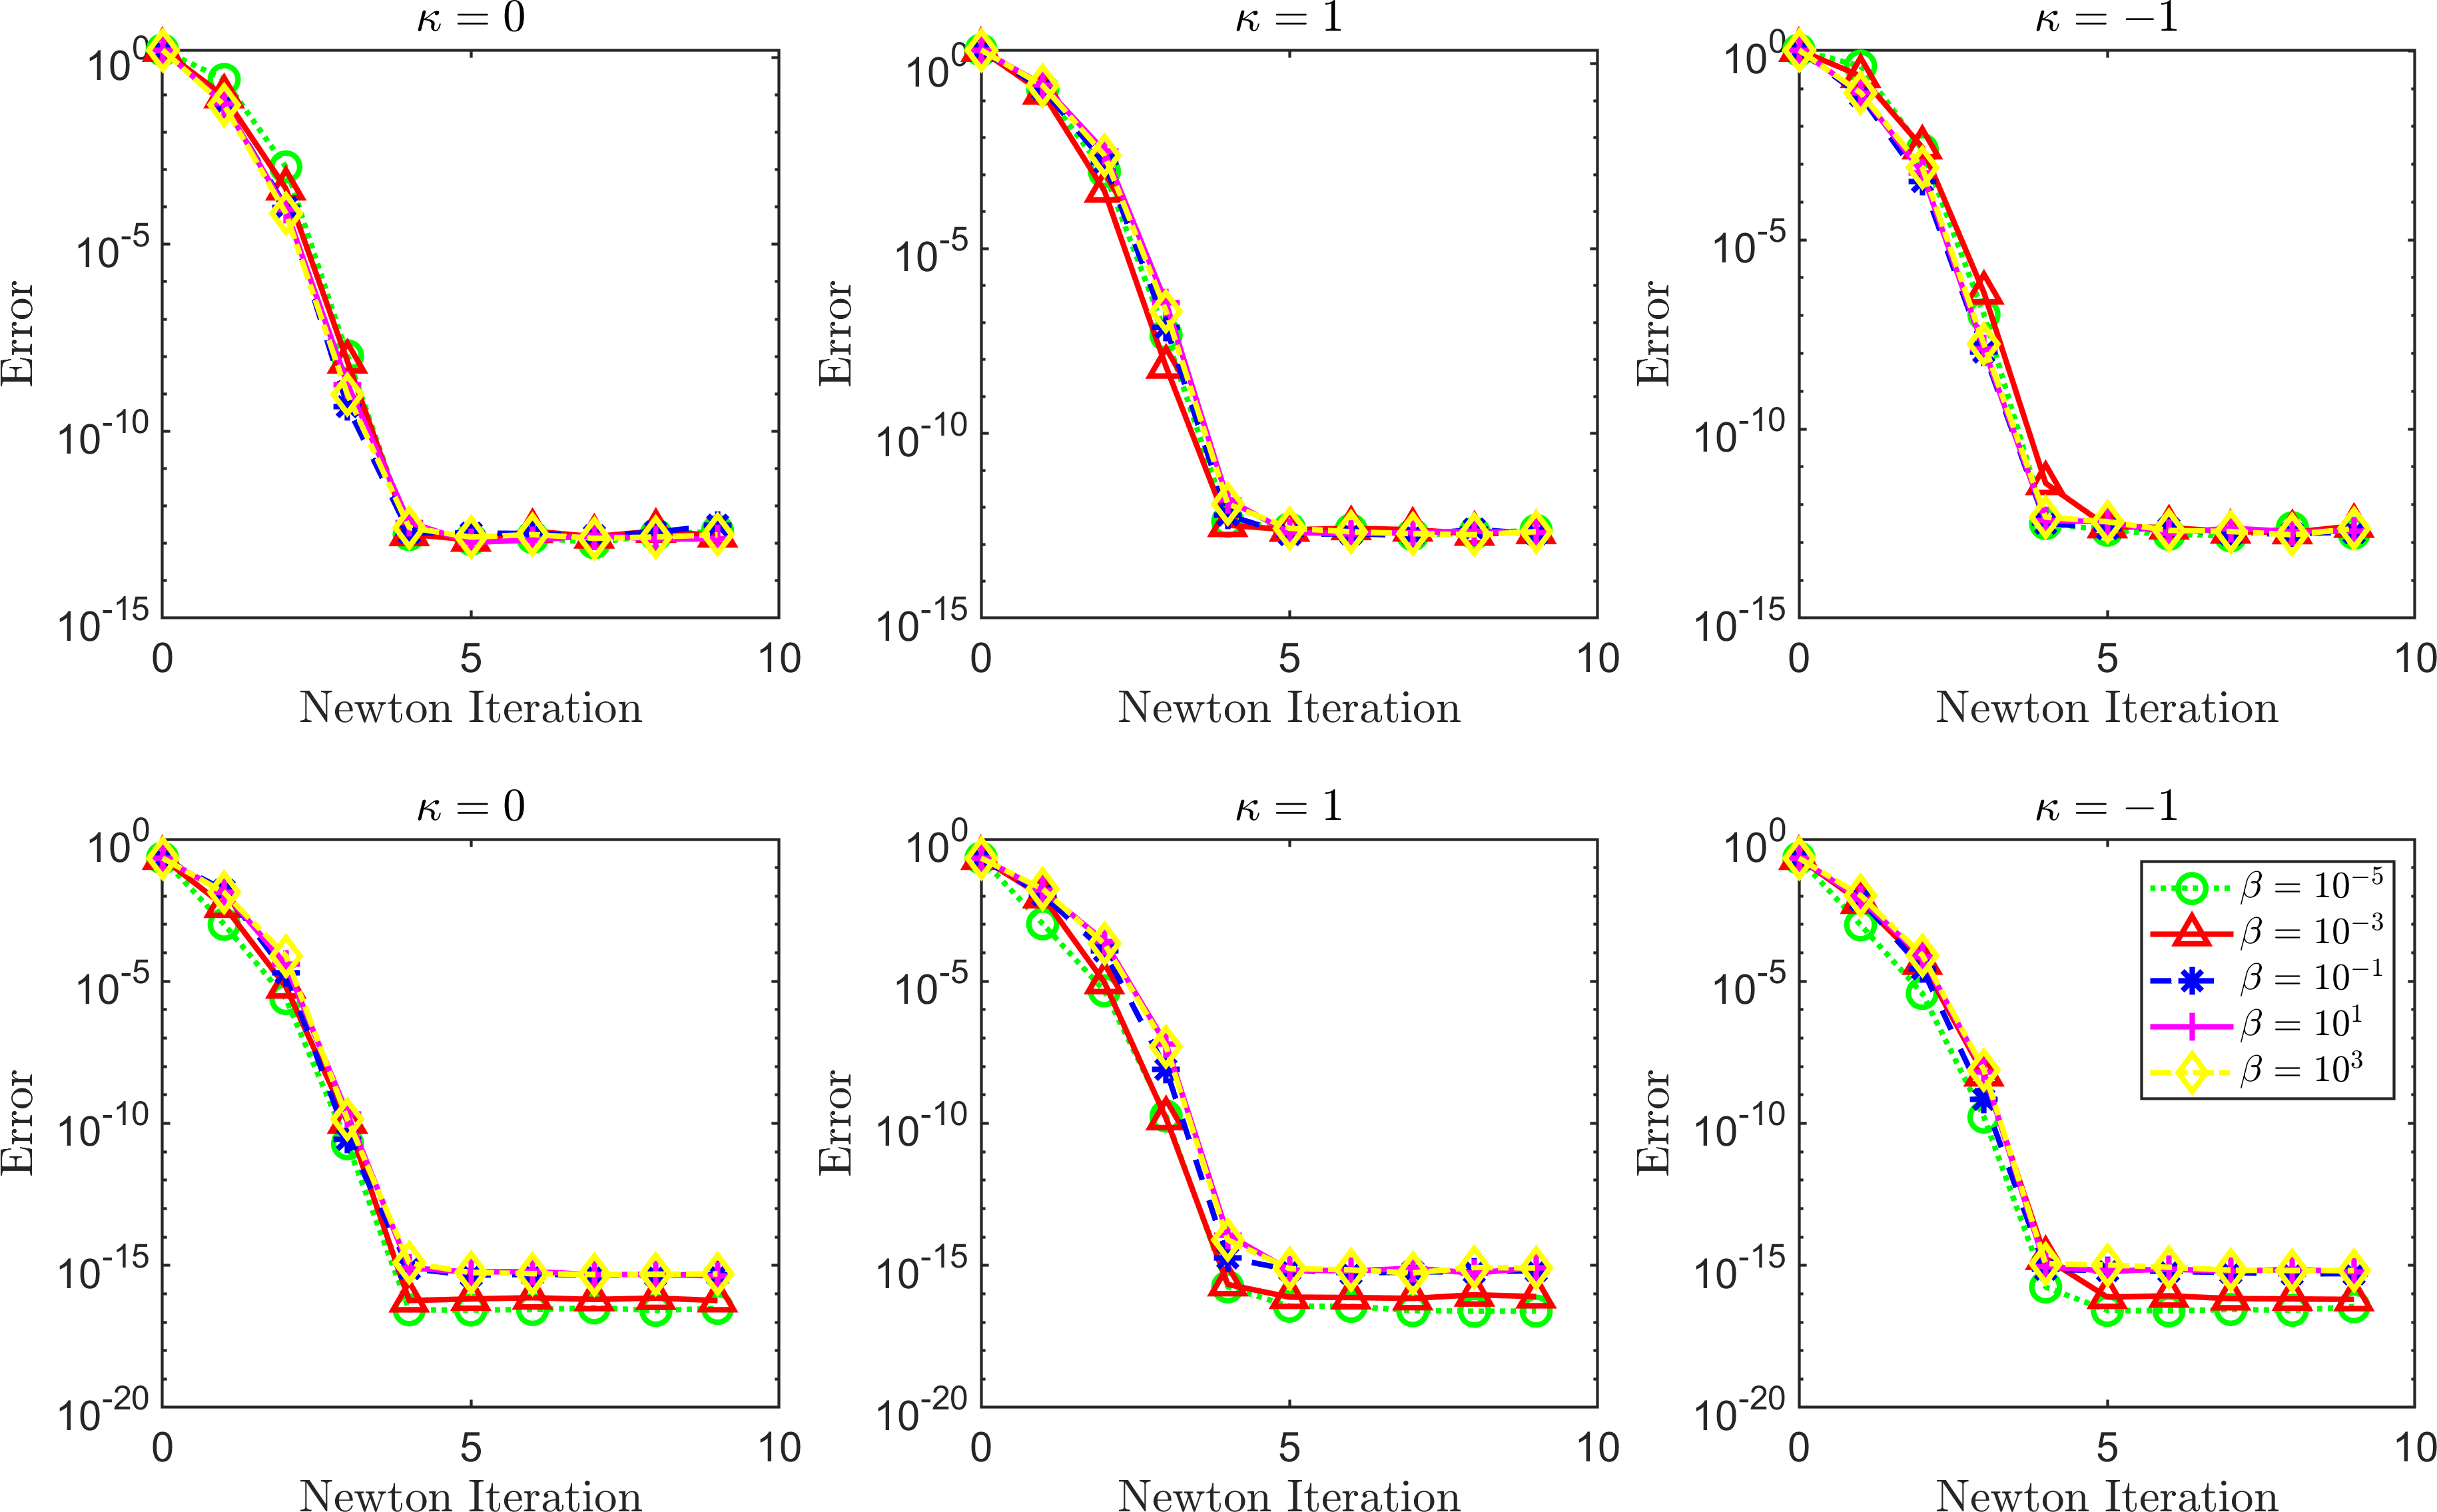
\includegraphics[scale=0.1]{SCDConvergence.png}
	\caption{Convergence of the Newton-Krylov Algorithm for Dirichlet source control. Top three plots show the convergence in the state variable for different $\kappa$, while the bottom plots show the convergence in the adjoint variable.} 
	\label{Con2}
\end{figure}
\begin{figure}[h]
	\centering
	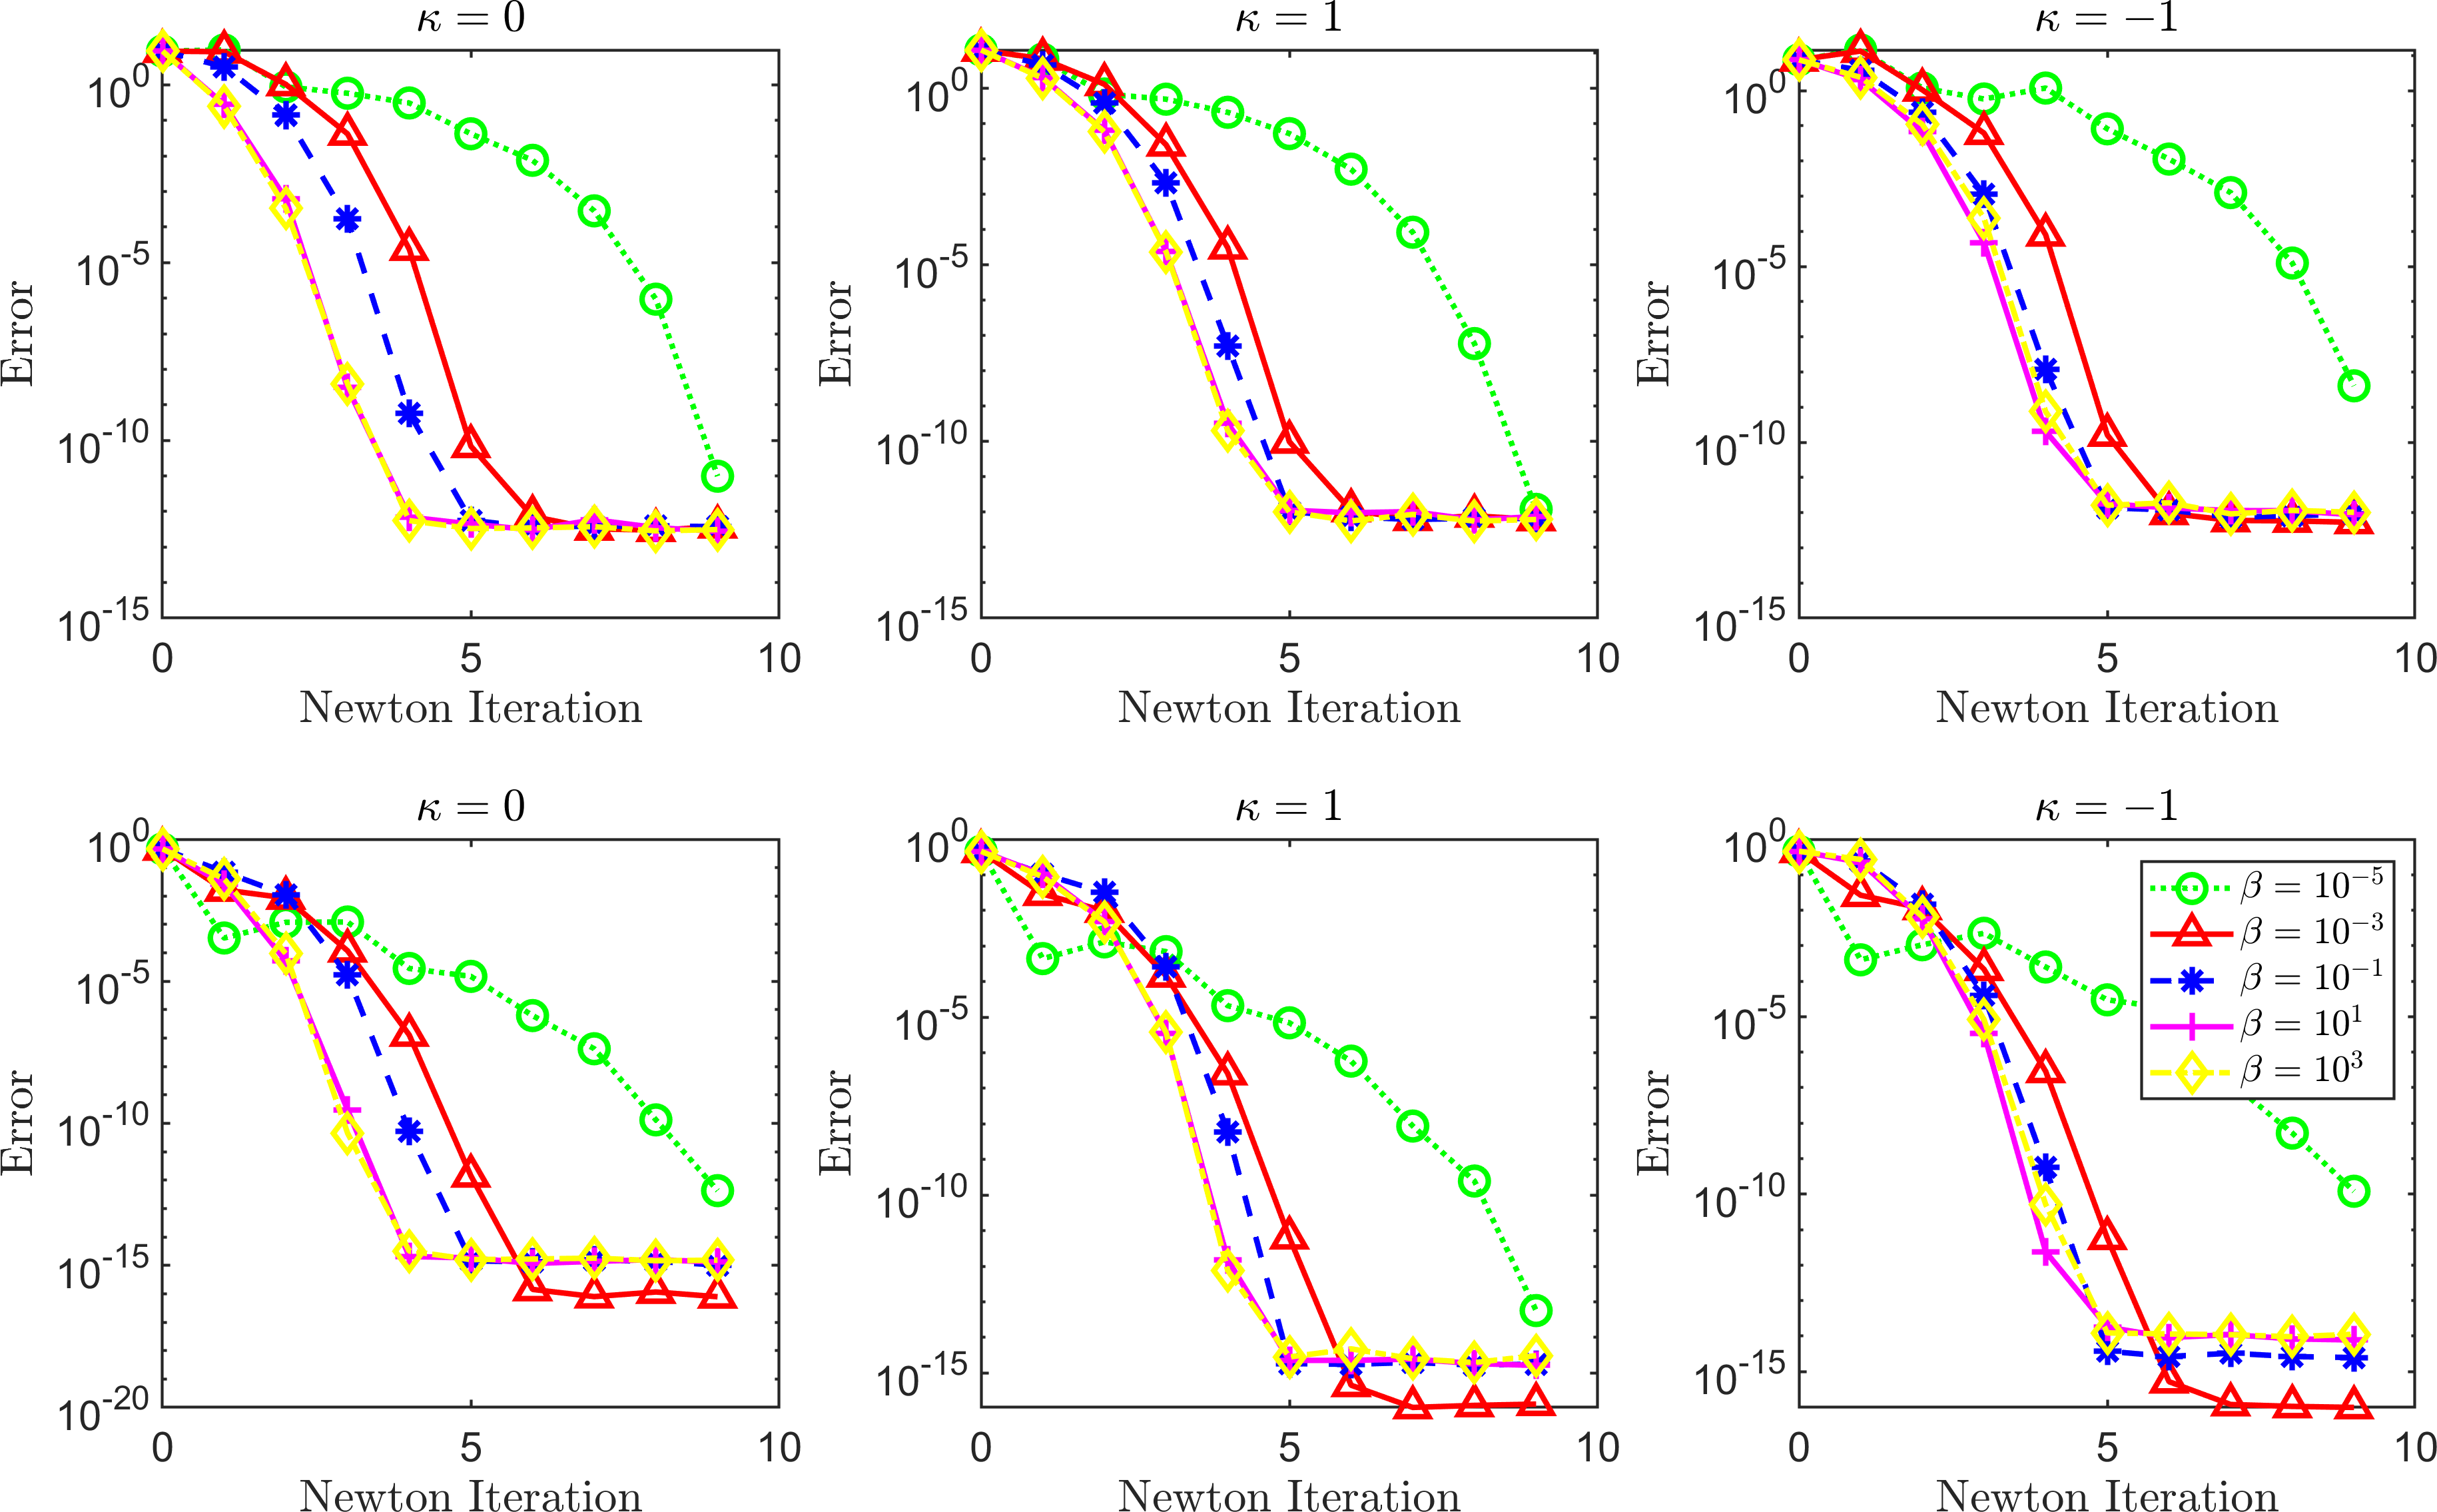
\includegraphics[scale=0.1]{FCDConvergence.png}
	\caption{Convergence of the Newton-Krylov Algorithm for Dirichlet flow control. Top three plots show the convergence in the state variable for different $\kappa$, while the bottom plots show the convergence in the adjoint variable.} 
	\label{Con3}
\end{figure}
\begin{figure}[h]
	\centering
	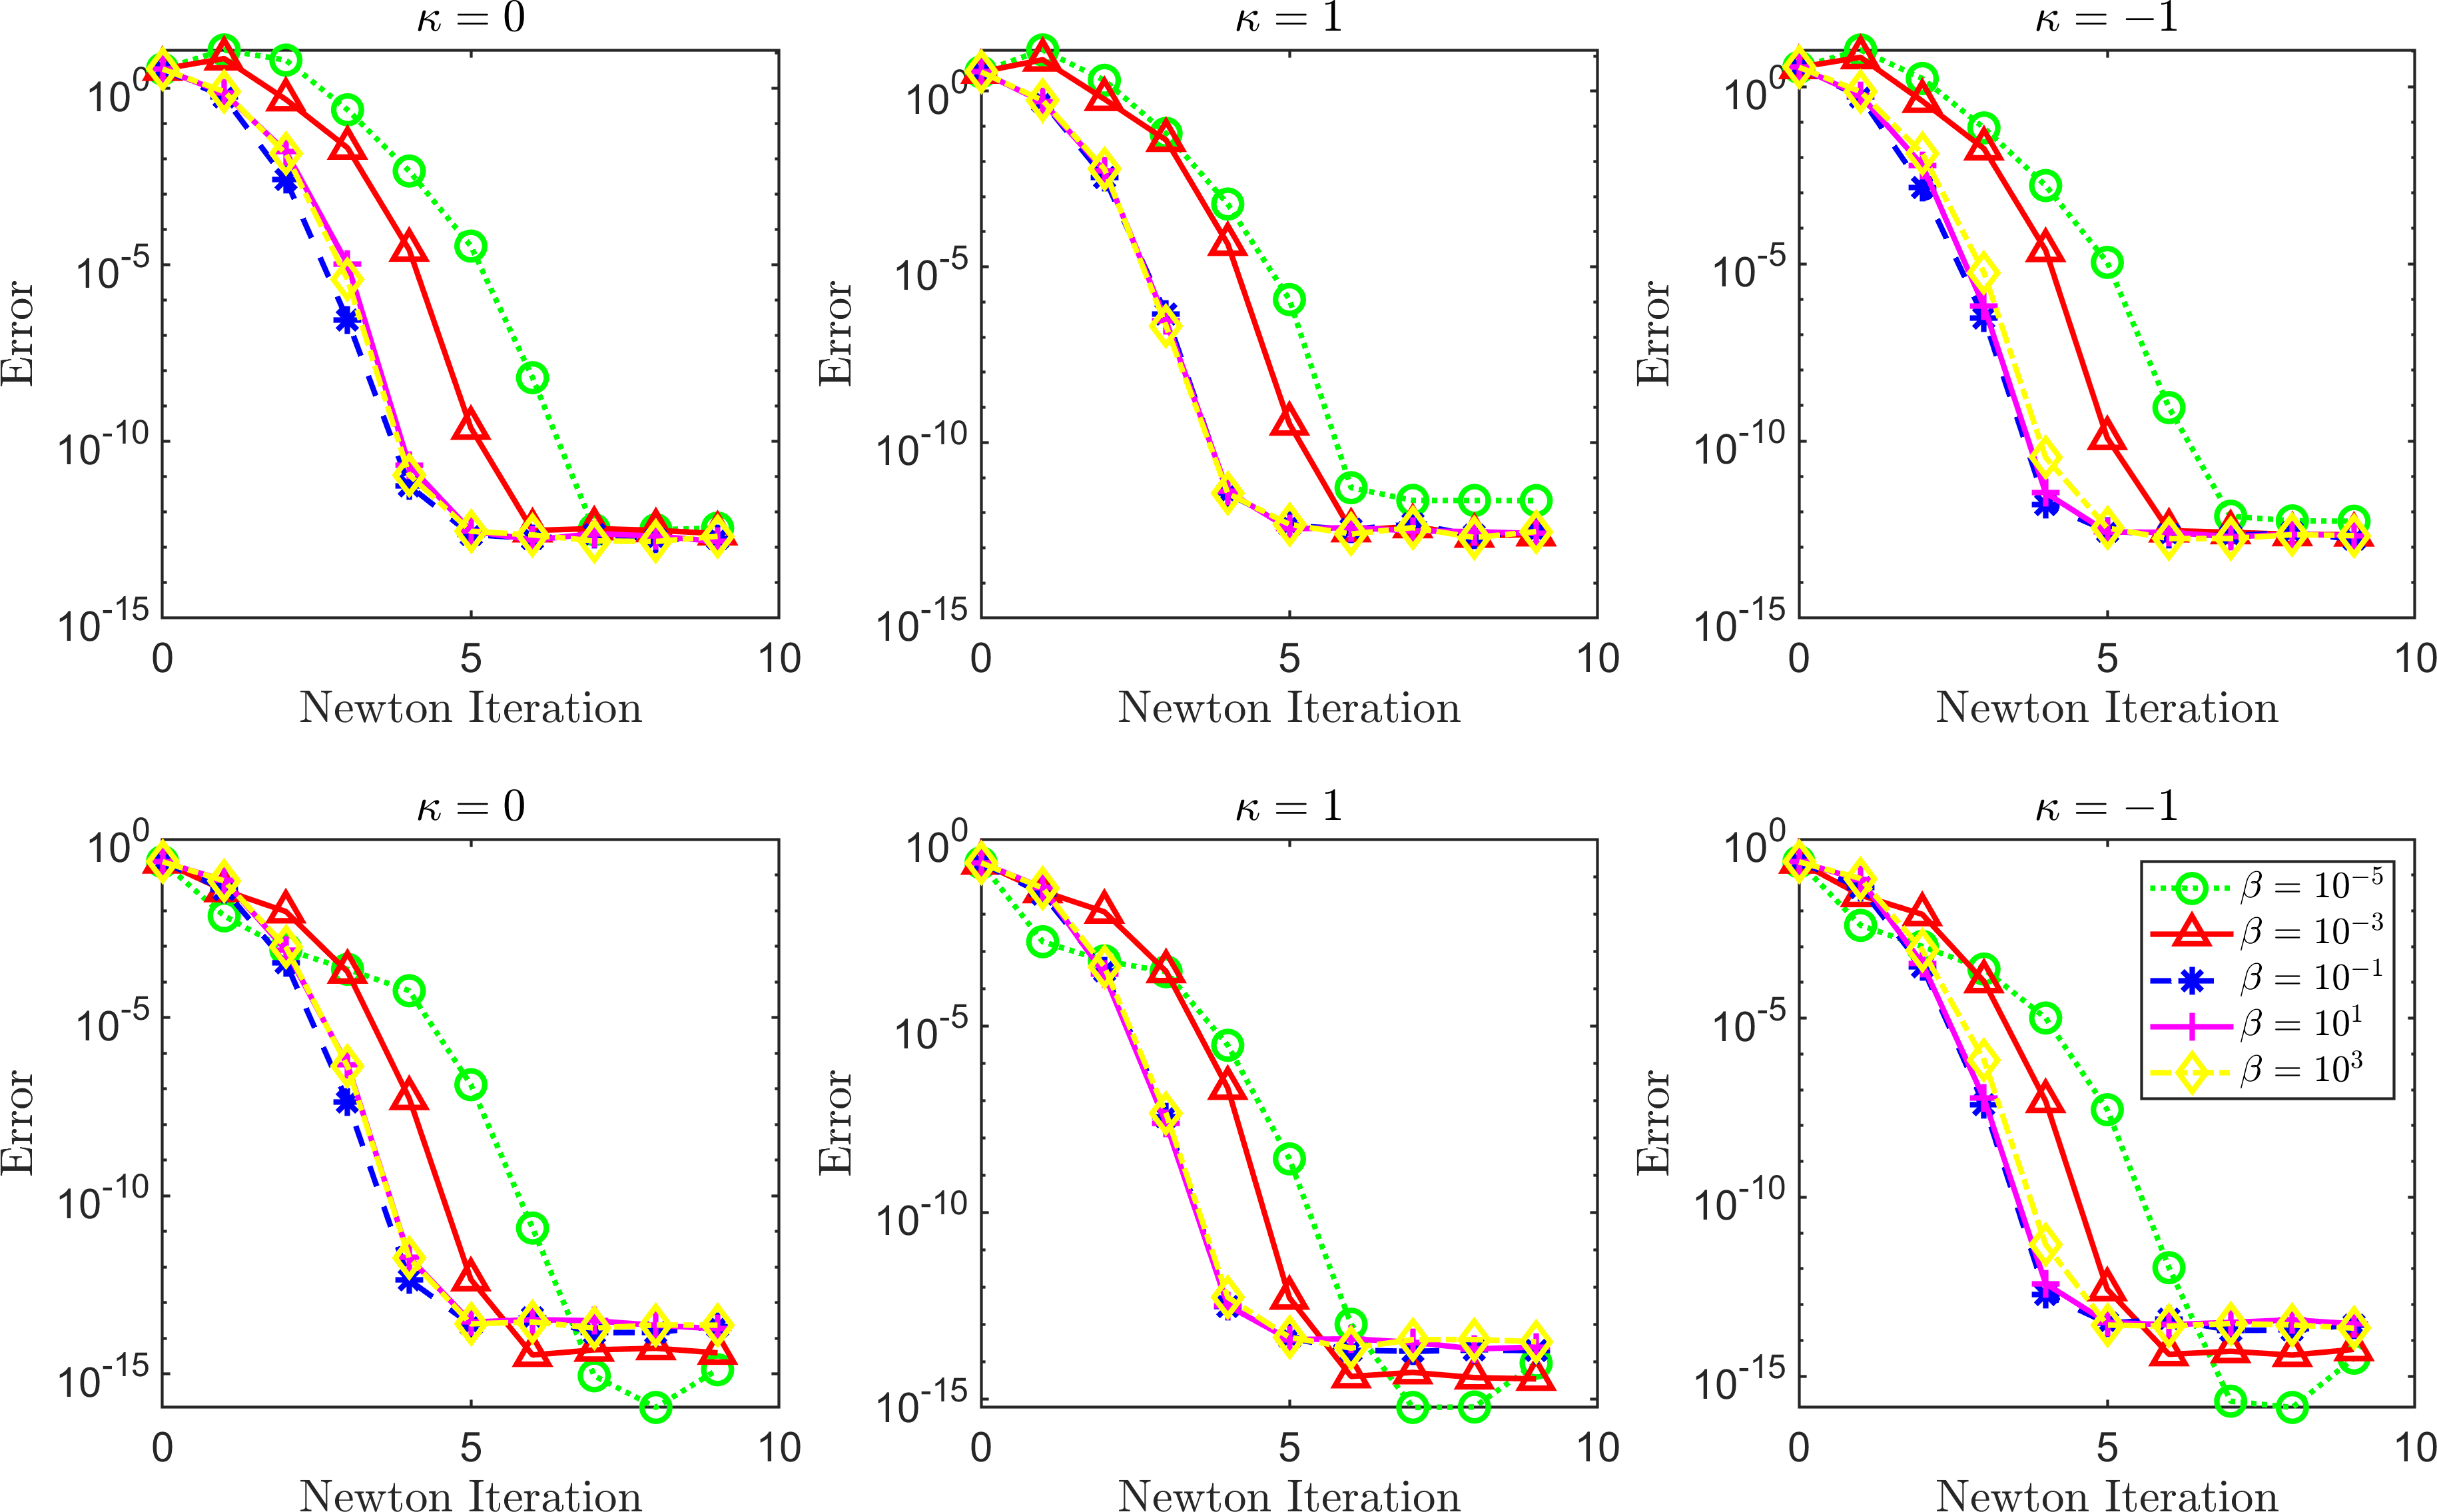
\includegraphics[scale=0.1]{FCNConvergence.png}
	\caption{Convergence of the Newton-Krylov Algorithm for no-flux flow control. Top three plots show the convergence in the state variable for different $\kappa$, while the bottom plots show the convergence in the adjoint variable.} 
	\label{Con4}
\end{figure}